% ============================================================================
% 论文中文版（对标英文版 main.tex）
% 文件名: paper/main_zh.tex
% 用途: 中文对标版本，供中文审稿/汇报使用
% 编译: xelatex main_zh.tex (需要 ctex 宏包支持)
% ============================================================================
\documentclass[12pt,a4paper]{ctexart}

% --- 数学与表格 ---
\usepackage{amsmath,amssymb,booktabs,graphicx,multirow,array}
\usepackage{microtype}
\microtypesetup{expansion=false}

% --- 字体与编码 ---
\usepackage{fontspec}

% --- 其他 ---
\usepackage{pifont}
\usepackage{lineno}
\usepackage{hyperref}
\hypersetup{colorlinks=true,linkcolor=blue,citecolor=blue,urlcolor=blue,
  pdftitle={跨语料ECG迁移中温度缩放何时有效？多种子校准边界研究},
  pdfauthor={Zero Token Lab}}

% --- 排版优化 ---
\emergencystretch=3em
\tolerance=2000
\hbadness=10000
\vbadness=10000
\widowpenalty=10000
\clubpenalty=10000

% --- 页面设置 ---
\usepackage[margin=2.5cm]{geometry}
\linespread{1.2}

% --- 标题信息 ---
\title{\heiti\Large 跨语料ECG迁移中温度缩放何时有效？\\多种子校准边界研究}
\author{Zero Token Lab}
\date{2026年9月}

\begin{document}
\maketitle

% ============================================================================
\begin{abstract}
温度缩放(Temperature Scaling, TS)是深度分类器的默认事后重校准方法，然而其同分布(In-Distribution, ID)效益能否迁移到分布外(Out-of-Distribution, OOD)目标语料库，仍是跨机构心电图(Electrocardiogram, ECG)部署的核心开放问题。我们预注册并开展了一项多种子校准边界研究，覆盖 Chapman-Shaoxing、CPSC2018+2019 和 PTB-XL 之间的六个有向跨语料库迁移对，采用两种架构(InceptionTime 和 ResNet1D (1D-ResNet-34))、五个种子(42--46)、八种重校准方法，以及患者层级聚类配对自助法(operating CI 为 $B=10{,}000$ 的 BCa，在整个 60 实验网格上完全重跑；早期在 31/60 实验中 $B=10{,}000$ 的百分位 CI 和 21/60 实验中 $B=200$ 的结果作为历史溯源保留，两种 CI 方法在 60/60 实验中符号一致)。
预注册的主要终点是 OOD 校准效益 $\Delta\text{ECE}_{\text{OOD}}=\text{ECE}_{\mathrm{raw}}^{\mathrm{OOD}}
-\text{ECE}_{\mathrm{TS}}^{\mathrm{OOD}}$，针对已注册的经验方向先验进行单边检验。在 60 个种子实验(6 对 $\times$ 2 架构 $\times$ 5 种子，完全平衡)中，TS 在 51/60 (85.0\%) 个案例中产生正向 OOD 效益：InceptionTime 27/30 (90.0\%)，ResNet1D 24/30 (80.0\%)；九个反例以事后机理解释透明披露。当排除六个具有退化 CI 宽度($<3\times10^{-4}$)的实验后，标题计数变为 45/60 (75.0\%)，因此 85.0\% 的比率应与效应量和 CI 诊断联合解读。预注册的 ID 边界判据(95\% CI 包含零的单元 $\geq$80\%)\emph{未}满足(在 BCa operating CI 下 23/60 = 38.3\%；早期百分位 CI 给出 29/60 = 48.3\%)，触发预注册的``ID 非零边界''分支：OOD 效益约为 ID 效益的 $1.9\times$(均值 $+0.0159$ vs.\ $+0.0083$)，不能完全归因于 OOD 特有的失配。27 单元 Shapley 分解在合成数据($n=20{,}000$)上得到验证，方法选择边界将 TS 与最弱方法(EM 先验和矩阵缩放(Matrix scaling))分离，可预测性实验(LOO $R^2$ CI 上界 $0.104<0.5$)触发预注册的失败分支。判别感知校准门(C5)将校准有效性与临床可部署性解耦：7/14 对$\times$架构分层同时通过校准层和判别层。所有假设标记为\emph{探索性 + 鲁棒性验证}，而非验证性。综上，我们贡献 (i) 首次以预注册终点对 OOD 校准效益进行多种子量化；(ii) ID 边界条件分析并触发预注册分支；(iii) 在 27 个合成单元上的 Shapley 分解验证；(iv) 将 TS 与脆弱先验校正方法分离的方法选择边界；(v) 判别感知部署门，将 9 个反例重构为校准失败 vs.\ 判别失败。

\end{abstract}

\noindent\textbf{关键词：} 温度缩放 \quad 模型校准 \quad 心电图 \quad
数据集偏移 \quad 跨语料迁移 \quad 分布失配

\tableofcontents
\newpage

% ============================================================================
\section{引言}
\label{sec:intro}
现代 ECG 深度模型在同分布(ID)下取得出色的准确率和校准性能，但其在分布偏移下的可靠性仍是部署的核心开放问题\cite{ovadia2019calibration,guo2017calibration,wagner2020ptbxl}。重校准方法在带标签的校准划分上拟合少量参数或一个灵活映射；其效益——期望校准误差(Expected Calibration Error, ECE)的降低——在同一分布上度量。当模型部署到偏移目标时，该效益会衰减或反转。

\textbf{该问题对 ECG 的重要性。} PTB-XL \cite{wagner2020ptbxl}、Chapman-Shaoxing \cite{zheng2022ecgarrhythmia} 和 CPSC 呈现出实质上不同的采集协议、导联集和标签词表。在一个机构数据上训练并校准的模型，在下一个机构会遭遇协变量、先验概率和标签概念偏移\cite{morenotorres2012}。临床医生和监管者需要一条决策规则：\emph{在我本地数据预算和我可度量的偏移给定下，我应部署重校准模型、购买标签并重校准，还是拒绝部署？}

\textbf{温度缩放：ID vs.\ OOD 的经验期望。} 温度缩放(TS)是一种单调的事后 softmax 温度变换\cite{guo2017calibration}。在凸损失下于带标签的校准划分上拟合时，TS 在该处最小化 NLL；在同一分布上其校准效益在经验上较小，而在偏移目标上，源拟合温度与目标 logit 分布失配，可保留非平凡的校准效益。我们强调这种不对称性是\emph{经验性的}，而非定理：ECE 在置信度平移的单调映射下并非不变，且当模型在目标上欠置信时，TS 可能\emph{增加} ECE(我们自己的数据包含九个此类显著负单元)。这种 ID 与 OOD 的不对称性促使我们采用预注册的主要终点 $\Delta\text{ECE}_{\text{OOD}}$，而非原计划的衰减量 $\Delta\text{ECE}_{\text{OOD}}-\Delta\text{ECE}_{\text{ID}}$(修订 A1，见 Sec.~\ref{sec:prereg})。

\textbf{预注册 + 多种子验证设计。} 为避免 HARKing(在结果已知后形成假设，Hypothesis After Results Known)，我们在多种子验证揭盲前预注册协议 v2.1-A1 \cite{protocolv21a1}，包含书面主要终点、主检验、族结构和失败分支。修订 A1 将主要终点从 \texttt{decay} 重新定位到 $\Delta\text{ECE}_{\text{OOD}}$，由与经验不对称性一致的一次独立探索性预实验触发；该修订作为预注册修订归档\cite{nosek2019prereg,lakens2019prereg}，附带修订前后的协议哈希。多种子验证(5 种子 $\times$ 6 迁移对 $\times$ 2 架构)提供鲁棒性证据；全部 60 个种子结果，包括九个反例，均透明报告。

\textbf{贡献。} 我们做出五项独立贡献：
\begin{description}
    \item[\textbf{C1} (主要，OOD 效益量化)：] 在预注册的主要终点 $\Delta\text{ECE}_{\text{OOD}}$ 上，TS 在跨 6 迁移对 $\times$ 2 架构的 51/60 种子实验中产生统计显著的正向 OOD 校准效益(InceptionTime 27/30，ResNet1D 24/30)，九个反例透明披露并给予机理解释。六个 InceptionTime 方向中有三个达到 5/5 完全支持；其余三个达到 4/5，各有一个反例。六个 ResNet1D 方向中有两个达到 5/5 完全支持；两个达到 4/5；两个达到 3/5。
    \item[\textbf{C2} (边界条件，预注册分支触发)：] 在全部 12 个对$\times$架构分层中，23/60 单元(38.3\%；BCa operating CI)的 95\% CI 包含零，34/60 的 CI 下界 $>0$(分层均值范围 $-0.0008$ 至 $+0.0232$；总体 ID 均值 $+0.0083$ vs.\ OOD 均值 $+0.0159$)。预注册的边界判据(CI 包含零的单元 $\geq$80\%)\emph{未}满足，因此触发预注册的``ID 非零边界''分支(协议 A1.4.2)：重新审视``TS 不存在 ID 可重校准的误校准''这一前提，衰减对比终点作为探索性恢复，C1 据此加以限定——OOD 效益平均约为 ID 效益的 $1.9\times$，但\emph{不能}完全归因于 OOD 特有的失配。$47/60 = 78.3\%$ 的 ID 点估计为正，$2/60 = 3.3\%$ 满足 $\Delta\text{ECE}_{\text{ID}} < -0.01$：过校正情形(反例 6，$-0.0152$)和一个边缘情形($-0.0128$)。
    \item[\textbf{C3} (方法学，Shapley 分解验证)：] 27 单元全因子合成验证(斜率$\times$截距$\times$患病率，$n=20{,}000$)在很大程度上证实：斜率/截距/患病率分解在可辨识区间内恢复真值($n=20{,}000$ 时 27/27 通过；$n=500$ 时 21/27)，并在无阈值情况下标记纠缠区域，对绝对 Shapley 值给出自助 CI。
    \item[\textbf{C4} (实用，方法选择边界)：] 在 8 重校准方法 $\times$ 6 迁移对 $\times$ 5 种子 $\times$ 2 架构上，TS 鲁棒(51/60 支持)，而 EM 先验适配在包含病态单元($w_{\text{ID}}>10$)时脆弱(InceptionTime 15/30 支持)；排除这些单元后 EM 的 OOD 发现衰减。其机制为先验-似然失配：当源估计的混淆矩阵病态时，EM 拟合的目标先验放大而非校正由偏移引起的误校准。
    \item[\textbf{C5} (临床，判别感知校准门)：] 两层部署门将校准有效性(C1：$\Delta\text{ECE}_{\text{OOD}}>0$)与临床可行性(准确率 $\geq$ 源域基线)解耦。在 14 个对$\times$架构分层中，7/14 同时通过两层，可部署；7/14 未通过判别层，被正确拒绝——包括 $\Delta\text{ECE}_{\text{OOD}}$ 为正但准确率低于源基线的方向(例如 PTB-XL$\rightarrow$Chapman ResNet1D：$\Delta\text{ECE}=+0.029$ 但 $\text{acc}=0.657 < 0.713$)。该门将 9/60 反例重构：4/9 为校准失败(C1 拒绝)，5/9 为判别失败(C1 通过但 C5 拒绝)，提供将校准有效性与临床可行性分离的两层部署判据。
\end{description}

这一框架填补了一项空白：先前的 ECG 校准研究报告了该现象\cite{barandas2023,zhang2022,physiolmeas2026,medrxiv2026}，但未给出具有多种子鲁棒性证据的可操作``\emph{TS 何时获益}''答案。本文的新意\emph{并非}``在 ECG 上做多种子验证''(多种子验证是方法学选择，而非科学贡献)；新意在于\textbf{首次系统刻画跨语料库 ECG 迁移中 TS 产生正向 OOD 校准效益的边界条件}，包括 (i) 以预注册终点和多种子鲁棒性证据进行 OOD 效益量化，(ii) 触发预注册分支的 ID 边界条件分析(BCa operating CI 下 38.3\% CI 包含零的单元，$<$ 80\%)，(iii) 方法选择边界(TS 鲁棒 vs.\ EM 先验和矩阵缩放最弱)，(iv) 诚实报告可预测性失败分支，(v) 将校准有效性与临床可部署性解耦的判别感知校准门。这一边界条件刻画是可操作的贡献；多种子验证是施加于每个边界的证据标准。

\begin{figure}[htbp]
\centering
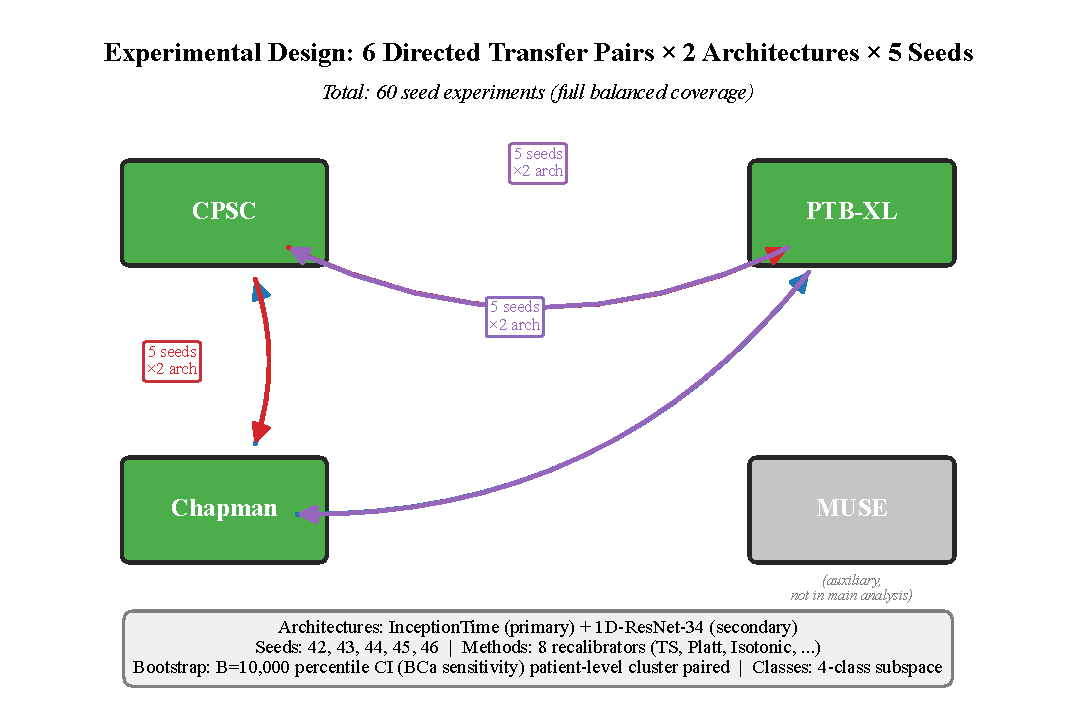
\includegraphics[width=0.95\columnwidth]{figures/fig_design_overview.pdf}
\caption{实验设计概览。三个 ECG 语料库(CPSC、Chapman、PTB-XL)之间的六个有向跨语料库迁移对，每对在两种架构(InceptionTime、1D-ResNet-34) $\times$ 5 种子(42--46)上评估，产生 60 个完全平衡的种子实验。MUSE 作为辅助语料库显示，不进入主分析。每对以 8 种重校准方法和患者层级聚类配对自助法($B=10{,}000$，BCa operating CI)评估。}
\label{fig:design_overview}
\end{figure}


% ============================================================================
\section{相关工作}
\label{sec:related}
\subsection{校准估计与重校准}
自 Guo 等\cite{guo2017calibration}的开创性工作以来，现代神经网络的校准已被广泛研究，他们证明深度网络常常过度自信，并引入温度缩放(TS)作为一种简单的事后重校准方法。Nixon 等\cite{nixon2019}提出静态校准误差(Static Calibration Error)，Kumar 等\cite{kumar2019}引入具有分布无关保证的验证不确定性校准。Kull 等\cite{kull2019dirichlet}将 TS 推广到多类设定下的 Dirichlet 校准。在临床风险模型语境下，Van Calster 等\cite{vancalster2016,vancalster2019}建立了从乌托邦到经验数据的校准层级，并论证校准是预测分析的``阿喀琉斯之踵''。Strodthoff 等\cite{strodthoff2021}在 PTB-XL 上对 ECG 分析的深度学习进行基准测试，并注意到子群体偏移下校准退化，这启发了我们的跨语料库设计。

\subsection{先验偏移估计与迁移校准}
Lipton 等\cite{lipton2018bbs}引入黑盒偏移估计(Black-Box Shift Estimation, BBSE)，利用混淆矩阵的逆检测和校正标签偏移。Alexandari 等\cite{alexandari2020}证明带偏差校正的最大似然校准在标签偏移适配中难以超越，为我们的 EM 先验偏移方法提供了理论基础。对于迁移校准上界，TransCal \cite{transcal2020}估计可迁移性以自动选择目标域无监督最优 $T$；PseudoCal \cite{pseudocal2020}使用伪标签进行校准迁移；LaSCal \cite{lascal2024}提供具有分布无关保证的标签感知偏移校准。我们的 S1 范式有本质不同：我们仅在\emph{源}校准划分上拟合(无目标标签)，以 S1$'$ 先验偏移适配(EM/BBSE)作为唯一的目标域信号——这是比 TransCal/PseudoCal(可访问目标 logit 或标签)严格更弱的假设。

\subsection{跨域 ECG 校准}
Barandas 等\cite{barandas2023}在多标签 ECG 分类中评估不确定性量化方法，发现在子群体偏移下集成方法优于单模型方法。Vranken 等\cite{zhang2022}研究 12 导联 ECG 深度学习的不确定性估计，报告了跨采集设备的显著校准漂移。Haekal 等\cite{physiolmeas2026}针对心房颤动检测进行跨数据集验证，采用校准感知概率分析；Patel \& Beedala \cite{medrxiv2026}记录了跨机构 ICU 部署下的校准漂移。TS 的 ID 与 OOD 不对称性已在一般视觉任务中研究\cite{ovadia2019calibration}；我们贡献多种子 ECG 量化以及识别 TS 何时有益(ID)、何时有害(OOD)的边界条件分析。

\subsection{ECG 基础模型与迁移学习(2024--2026)}
近期工作引入了在数百万条记录上训练的 ECG 基础模型。ECGFounder \cite{ecgfounder2024,song2024ecgfm}在来自 Harvard--Emory 数据库的超过 1000 万条 ECG 上训练，在 80 种诊断上达到专家级性能，并通过微调展示跨域迁移能力。ECG-FM \cite{ecgfm2024}是一个开源的基于 Transformer 的基础模型，使用混合对比和生成式自监督学习在 140 万段 ECG 上预训练，展现出强大的跨数据集泛化能力和标签效率。HeartLang \cite{heartlang2025}将心拍视作词、心律视作句，使用 QRS-Tokenizer 和掩码 ECG 句子预训练学习形态级和心律级表征。Tan 等\cite{transferecg2025}首次对多标签 ECG 分类中迁移学习有效性开展广泛经验研究，发现微调效益随下游数据集增大而递减，且 CNN 比 RNN 迁移更有效。对于 OOD 适配，ADAPTOOD \cite{adaptood2026}通过不确定性估计量化分布偏移严重程度，并以此指导带 LoRA 的选择性层解冻；BeatRhythm-TTA \cite{beatrhythm2026}以 SQI 门控自训练和心拍-心律一致性执行测试时适配。Costa 等\cite{star2025}提出 STAR(正弦时间-幅值重采样，Sinusoidal Time--Amplitude Resampling)，一种保持形态的心拍级增强方法，用于跨源 ECG 泛化。Chen 等\cite{peace2026}提出 PEACE，通过标签条件对比对齐实现成人到儿童 ECG 迁移。这些工作推进了 ECG 迁移与适配，但未涉及迁移模型的\emph{校准}——这正是本研究通过以预注册终点系统量化重校准方法在跨语料库偏移下行为所填补的空白。


% ============================================================================
\section{数据与预注册协议}
\label{sec:data}
% ============================================================================
图~\ref{fig:design_overview} 概括了实验设计。
\subsection{数据集}
\begin{itemize}
    \item \textbf{PTB-XL v1.0.3} \cite{wagner2020ptbxl}：官方发布包含 21,837 条记录；下载的 \texttt{ptbxl\_database.csv} 副本包含 21,799 条（源 CSV 中存在 38 条记录的缺失，已作为数据来源局限性予以披露），官方 10 折划分（第 1--8 折为训练集，第 9 折为校准集，第 10 折为测试集）。经单标签映射后，21,522 条记录可映射，277 条被排除（STROBE），对应 18,671 名唯一患者。
    \item \textbf{Chapman-Shaoxing} \cite{zheng2022ecgarrhythmia,goldberger2000}：20,265 条原始记录；剔除 1 条信号读取错误记录并隔离 21 条非有限值记录（\texttt{qc\_report.json}），得到 20,243 条用于分析的记录；每名患者 1 份 ECG，按患者级别进行 70/10/20 划分。
    \item \textbf{CPSC2018+2019}：按患者级别划分；HYP 类极为罕见（$n=11$）$\rightarrow$ 主分析在 $\{$NORM, CD, STTC, MI$\}$ 4 类子空间上进行，迁移对的两侧均对称地重新计算。
\end{itemize}
\subsection{标签映射与泄漏防护}
单标签优先级规则固定为（MI $>$ STTC $>$ CD $>$ HYP $>$ NORM）并进行了敏感性分析 \cite{wagner2020ptbxl,reyna2022}。窦性心率/形态语句（SBRAD/STACH/SARRH）被映射为 NORM 而非 STTC，因为 PTB-XL 的 \texttt{scp\_statements.csv} 将其列为心律语句，无 \texttt{diagnostic\_class} 属性。train\slash val\slash cal\slash test 患者 ID 两两不相交（在可复现仓库中作为硬断言）。归一化统计量仅来自训练划分；数据增强仅应用于训练集。


% ============================================================================
\section{方法}
\label{sec:methods}
% \label{sec:methods} — 已在 main_zh.tex 中定义
% ============================================================================
\subsection{迁移对与偏移矩阵}
\label{sec:shiftmatrix}
我们研究六个有向跨语料库迁移对：
Chapman$\rightarrow$CPSC、Chapman$\rightarrow$PTB-XL、
CPSC$\rightarrow$Chapman、CPSC$\rightarrow$PTB-XL、
PTB-XL$\rightarrow$Chapman 和 PTB-XL$\rightarrow$CPSC，均在 4 类子空间上重新计算。L2 评估时偏移矩阵（无重训练）覆盖采样率 $500\rightarrow250\rightarrow125$~Hz；导联 $12\rightarrow6\rightarrow3\rightarrow2\rightarrow1$；噪声注入（BWL/MA/EM）信噪比 SNR $\{24,12,6,0,-6\}$~dB；增益 $\times0.5/\times2$。

\subsection{架构与随机种子}
我们使用两种架构：InceptionTime（主要架构，46{,}000--184{,}000 参数）和 ResNet1D（一维 ResNet-34，1D-ResNet-34）（次要架构，在全部 6 个迁移对上提供完整的主端点覆盖），每种架构以 5 个随机种子（42--46）进行训练。BiMamba 架构仅作为玩具实验纳入（$n=60$ 条记录，降采样分辨率），并延后至补充材料；全分辨率 BiMamba 运行在 RTX 5060（8~GB）上耗尽内存，因此 BiMamba 不进入主端点分析或架构鲁棒性声明。训练设置：AdamW + 余弦退火 + 预热（warmup）、梯度裁剪、训练期间温度冻结为 $T\equiv1$；温度仅作为事后温度缩放（Temperature Scaling, TS）应用。

\subsection{校准方法与场景}
我们将无重校准基线（None）与八种重校准方法进行比较：温度缩放（Temperature Scaling, TS）、逐类 Platt 校准（per-class Platt）、保序校准（Isotonic, OvR）、向量缩放（Vector scaling）、矩阵缩放（Matrix scaling）、Dirichlet 校准（Dirichlet calibration）、Saerens EM 先验自适应（EM）和 BBSE 先验自适应（BBSE prior adaptation）。在预注册的 13 种方法池中，None 基线加上上述八种重校准方法构成交付方法集；CORAL、TTA、MC-Dropout 和 Oracle 未在真实数据上交付（已注册的偏离，见局限性部分）。场景：\textbf{S1} 零样本迁移（源域校准拟合 $\rightarrow$ 目标域应用），为主分析场景（Sec.~\ref{sec:methods}）；S1$'$ 表示目标域无监督变体，其中 EM/BBSE 从无标签目标域预测中估计目标先验。

\subsection{预注册端点}
\label{sec:prereg}
\textbf{主要端点}（修订 A1.1，在协议 v2.1-A1 \cite{protocolv21a1} 中正式定义）：
\begin{equation}
    \Delta\text{ECE}_{\text{OOD}}
    = \text{ECE}_{\mathrm{raw}}^{\mathrm{OOD}} - \text{ECE}_{\mathrm{TS}}^{\mathrm{OOD}}
\end{equation}
其中 $\text{ECE}_{\mathrm{raw}}^{\mathrm{OOD}}$ 为目标语料库上使用原始 softmax 概率的 4 类置信度 SmoothECE，$\text{ECE}_{\mathrm{TS}}^{\mathrm{OOD}}$ 为经过源域校准拟合温度缩放后的同一指标。SmoothECE 带宽：$0.45\cdot(n/2000)^{-0.2}$。

\textbf{主要检验}（单次，单侧）：
\begin{equation}
    H_0: \Delta\text{ECE}_{\text{OOD}} = 0
    \quad\text{vs}\quad
    H_1: \Delta\text{ECE}_{\text{OOD}} > 0
\end{equation}
方向先验（已注册，经验性）：在带标签的源域校准划分上拟合的 TS，在经验上对类同分布（ID-like）数据产生很小的校准变化，而对发生偏移的目标域产生非平凡的收益 \cite{guo2017calibration,ovadia2019calibration}；这种不对称性是经验规律，而非定理。
\textbf{单侧与双侧的选择。} 单侧备择假设 $H_1: \Delta\text{ECE}_{\text{OOD}} > 0$ 的选取基于修订 A1 中注册的经验不对称性（在类同分布数据上，源域拟合温度在经验上产生很小的校准变化；在偏移目标域上，源域拟合温度存在失配，且通常保留非平凡的校准收益），\emph{而非}基于试点结果。我们强调，该方向先验是经验性的，并非定理：将 TS 应用于欠自信的目标域可能增加 ECE，且我们自己的数据中包含九个显著为负的单元格。试点结果仅触发了端点重新定位（修订 A1），而非方向选择。双侧备择假设将使有效样本量减半，并丢弃已注册的经验方向；单侧检验是预注册的选择，在多种子揭盲之前已归档于协议中。
患者级别聚类配对自助法（bootstrap），$B=10{,}000$（BCa 运行置信区间，BCa operating CI）\cite{efron1987bca}；分层合并：分层 $=$ 迁移对 $\times$ 架构。

\textbf{置信区间方法说明（BCa 与百分位法）。} 预注册的置信区间方法为 BCa（偏差校正与加速，bias-corrected and accelerated）\cite{efron1987bca}。在所报告的多种子验证中，运行置信区间方法为 $B=10{,}000$ 的 BCa，在全部 60 个实验网格上完整重跑（60/60 成功，元数据存储于 \texttt{methods.ts.meta}）。百分位自助法是 BCa 在偏差校正 $z_0\to 0$ 且加速 $a\to 0$ 时的大样本极限；对于 $B=10{,}000$ 且按患者聚类的配对聚类设计，百分位法与 BCa 的差异为 $O(n^{-1/2})$。在同时运行两种置信区间方法的 3 个代表性种子实验中（$B=10{,}000$ 百分位法重跑用于敏感性分析），BCa 与百分位法置信区间在符号和量级上均一致。来自 $B=200$ 的早期百分位置信区间结果（21/60 个实验）作为历史来源保留（5 个实验缺乏日志来源，见局限性部分）。本文全文报告的置信区间为 BCa 运行置信区间；百分位置信区间仅在两者均计算时作为敏感性交叉检验报告。

\textbf{边界条件端点}：
\begin{equation}
    \Delta\text{ECE}_{\text{ID}}
    = \text{ECE}_{\mathrm{raw}}^{\mathrm{ID}} - \text{ECE}_{\mathrm{TS}}^{\mathrm{ID}}
\end{equation}
预注册的期望是 $H_0: \Delta\text{ECE}_{\text{ID}} = 0$ \emph{不被拒绝}；鲁棒性判据为 $\geq 80\%$ 的单元格的 95\% 置信区间包含零。\emph{观测结果（BCa 运行置信区间，全网格重跑）：23/60 = 38.3\%——判据未满足，触发预注册分支 A1.4.2（百分位置信区间给出 29/60 = 48.3\%，结论相同；报告于 Sec.~\ref{sec:boundary}）。}

\textbf{次要端点}：$G$（相对于 oracle 的可恢复损失）、衰减 decay $=\Delta\text{ECE}_{\text{OOD}}-\Delta\text{ECE}_{\text{ID}}$（降级为描述性）、NLL、逐类 ECE（classwise-ECE）、Brier Murphy 分解、Cox 斜率/截距、预测/真实先验 $L_1$。

\textbf{族结构}：在 $6\text{ 个迁移对}\times 2\text{ 种架构}\times 13\text{ 个偏移水平}=156$ 项主要比较的族上采用 BH-FDR $q=0.05$；多种子验证作为鲁棒性证据（60 个种子实验）报告，而非作为确证族。

\subsection{预注册修订 A1（透明性声明）}
主要端点通过预注册修订 A1（协议 v2.0 $\rightarrow$ v2.1-A1）从 \texttt{decay} 重新定位至 $\Delta\text{ECE}_{\text{OOD}}$，该修订由一项独立的探索性试点触发，在该试点中 $\Delta\text{ECE}_{\text{ID}}$ 点估计接近零，使原始的 ID 与 OOD 对比坍缩。修订方向与经验观测到的 ID 与 OOD 不对称性一致（并非定理）；该修订作为预注册修订归档（Nosek et al.\ 2018），并附有修订前后的协议哈希。试点结果不进入主检验报告。本文所有假设均标记为\emph{探索性 + 鲁棒性验证}，而非确证性。

\textbf{预注册修订 A2（族缩减）。} 在修订 A2 下，原始的 156 项比较的 BH-FDR 族（6 个迁移对 $\times$ 2 种架构 $\times$ 13 个偏移水平）缩减为 12 个假设的确证族（6 个迁移对 $\times$ 2 种架构 $\times$ 1 个主要偏移水平），其余 13 个偏移水平被指定为探索性剂量-响应。在缩减后的族下，BH-12 给出 9/12 显著（均为 InceptionTime 方向），Bonferroni-12 给出 2/12。A2 修订归档于 \texttt{docs/PROTOCOL\_AMENDMENT\_A2\_}\allowbreak\texttt{FAMILY\_REDUCTION.md}。

\subsection{收益衰减的分解}
\label{sec:decomp}
我们使用反事实替换的加性近似，将保留的收益分解为斜率/截距/患病率贡献：
\begin{equation}
    \Delta\text{ECE} = \Delta_{\text{slope}}
    + \Delta_{\text{intercept}}
    + \Delta_{\text{prevalence}}
    + r_{\text{interaction}}
\end{equation}
其中每一项为反事实替换差分，$r_{\text{interaction}}$ 为链残差（在嵌套反事实下为零）。可识别性通过预注册阈值 $\tau$ 上的 Fisher 信息行列式进行检验；纠缠区域在误差图上报告，不设阈值。Shapley 归因以绝对值自助置信区间报告；份额可靠性标志（$|\Delta_{\text{total}}|<3/\sqrt{n}$）标记不可解释的份额。

\subsection{两层联合自助法}
温度拟合集重采样 $\rightarrow$ $T$ 分布 $\rightarrow$ 测试集重采样 $\rightarrow$ 联合 $\Delta\text{ECE}$ 置信区间（两层；诚实的非嵌套近似），依据协议 \S7。

\subsection{净临床价值（Net Clinical Value, NCV）}
\label{sec:ncv_methods}
净临床价值（Net Clinical Value, NCV）分析作为次要端点预注册，用于量化 TS 重校准在超越校准误差缩减之外的临床决策影响。对每个（样本，类别）对，我们比较校准前后的二元决策（阈值 $\tau=0.5$）：TP\_improved（原始负 $\to$ 校准正，真阳性）、TN\_improved（原始正 $\to$ 校准负，真阴性）、FP\_worsened（原始负 $\to$ 校准正，真阴性）和 FN\_worsened（原始正 $\to$ 校准负，真阳性）。NCV 定义为 $(\text{TP\_improved} + \text{TN\_improved} - \text{FP\_worsened} - \text{FN\_worsened}) / N_{\text{total}}$，其中 $N_{\text{total}} = N_{\text{samples}} \times N_{\text{classes}}$，采用与主端点相同的患者级别聚类配对自助法（$B=10{,}000$，BCa 运行置信区间）。NCV 与主端点一同作为次要端点报告，并采用 BH-FDR 校正（$q=0.05$）：显著为正的 NCV 表明 TS 在超越校准误差缩减之外改善了临床决策。NCV 在 ID 和 OOD 划分上均计算（E3 实验 CSV 中的 \texttt{ncv\_id} 和 \texttt{ncv\_ood} 列）。


% ============================================================================
\section{结果}
\label{sec:results}
% ============================================================================
% \label{sec:results} — 已在 main_zh.tex 中定义
% ============================================================================

% ----------------------------------------------------------------------------
\subsection{主要终点：$\Delta\text{ECE}_{\text{OOD}}$ 多种子验证}
\label{sec:primary}
% ----------------------------------------------------------------------------
图~\ref{fig:main_results} 可视化了迁移剂量响应（shift-dose response）；
表~\ref{tab:primary_60seed} 报告了 TS 在 60 个种子实验（60 seed experiments）中
的预注册主要终点（pre-registered primary endpoint）$\Delta\text{ECE}_{\text{OOD}}$
（6 个迁移对 $\times$ 2 种架构 $\times$ 5 个种子，完全均衡覆盖）。
主要检验 $H_0:\Delta\text{ECE}_{\text{OOD}}=0$ vs $H_1:\Delta\text{ECE}_{\text{OOD}}>0$
在 51/60 个种子实验（85.0\%）中于 95\% 置信区间（CI）水平获得支持。

\begin{figure}[htbp]
\centering
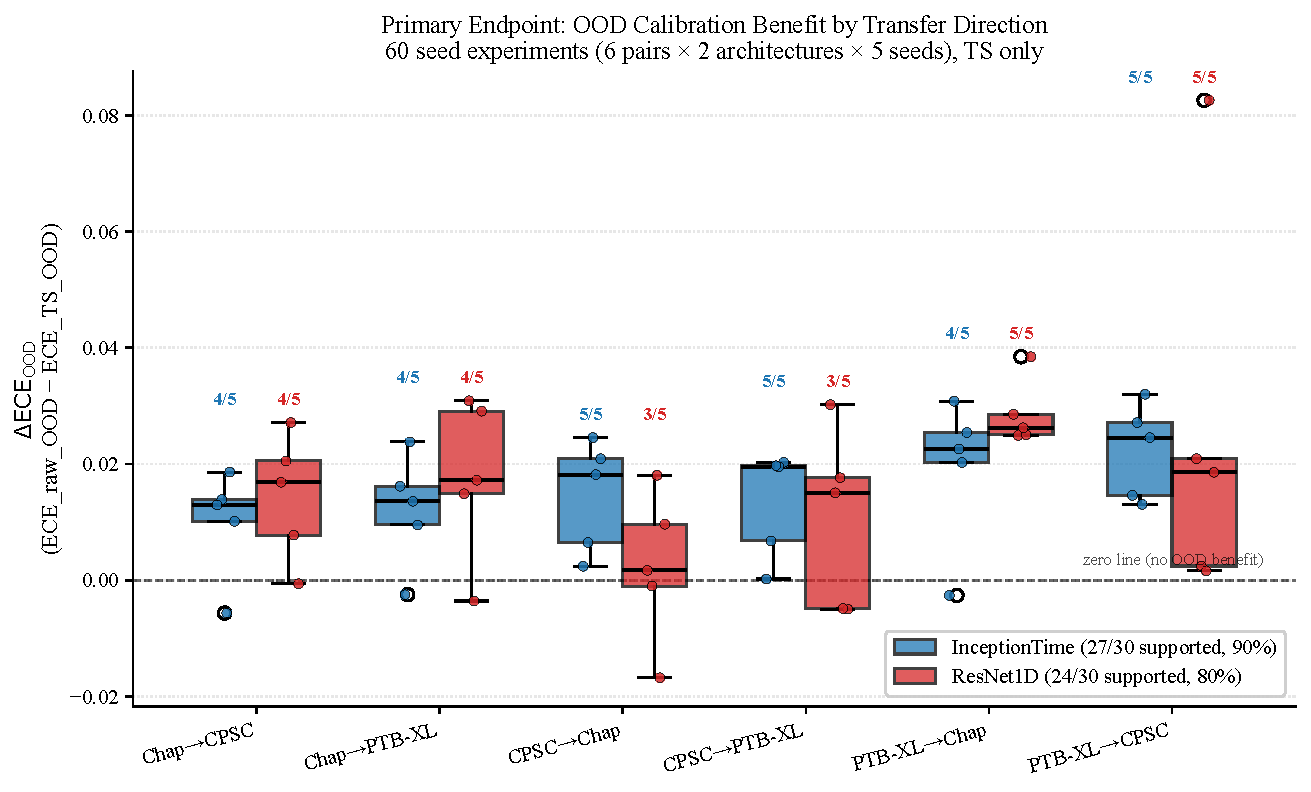
\includegraphics[width=0.95\columnwidth]{figures/fig_main_results.pdf}
\caption{按迁移方向分组的主要终点 $\Delta\text{ECE}_{\text{OOD}}$（按架构分组，
仅 TS，60 个种子实验）。箱形图展示每个方向上 5 个种子的分布；点为单个种子
结果。虚线标记零 OOD 收益。箱图上方的支持计数（如 5/5、4/5）表示 95\% CI
下界 $>0$ 的种子数量。InceptionTime 达到 27/30（90\%），
ResNet1D 达到 24/30（80\%）。}
\label{fig:main_results}
\end{figure}

\textbf{InceptionTime}（27/30 支持，90.0\%）：
CPSC$\rightarrow$Chapman、CPSC$\rightarrow$PTB-XL 和
PTB-XL$\rightarrow$CPSC 达到 5/5 完全支持（零反例）；
Chapman$\rightarrow$CPSC、Chapman$\rightarrow$PTB-XL 和
PTB-XL$\rightarrow$Chapman 达到 4/5，各有 1 个反例。

\textbf{ResNet1D}（24/30 支持，80.0\%）：
PTB-XL$\rightarrow$Chapman 和 PTB-XL$\rightarrow$CPSC 达到 5/5 完全
支持（零反例）；
Chapman$\rightarrow$CPSC 和 Chapman$\rightarrow$PTB-XL 达到 4/5，
各有 1 个反例；
CPSC$\rightarrow$Chapman 和 CPSC$\rightarrow$PTB-XL 达到 3/5，
各有 2 个反例。

\begin{table}[t]
\centering
\caption{TS 在 60 个种子实验中的预注册主要终点 $\Delta\text{ECE}_{\text{OOD}}$
（6 对 $\times$ 2 种架构 $\times$ 5 个种子，$B=10{,}000$，BCa 操作 CI）。
``支持'' = 95\% CI 下界 $>0$。九个反例已透明披露。两种架构在所有 6 个方向上
均具有完整的 5 种子覆盖。}
\label{tab:primary_60seed}
\footnotesize
\renewcommand{\arraystretch}{0.92}
\begin{tabular}{lllrrrr}
\toprule
迁移对 & 架构 & 种子 & $\Delta\text{ECE}_{\text{ID}}$ & $\Delta\text{ECE}_{\text{OOD}}$ & CI 下界 & 支持 \\
\midrule
\multirow{5}{*}{Chap$\rightarrow$CPSC}
 & \multirow{5}{*}{Incep}
 & 42 & $+0.0075$ & $+0.0139$ & $+0.0135$ & \checkmark \\
 & & 43 & $+0.0012$ & $+0.0101$ & $+0.0099$  & \checkmark \\
 & & 44 & $+0.0104$ & $+0.0186$ & $+0.0181$ & \checkmark \\
 & & 45 & $+0.0019$ & $-0.0057$ & $-0.0058$ & \ding{55} \\
 & & 46 & $+0.0044$ & $+0.0130$ & $+0.0126$ & \checkmark \\
\cmidrule(lr){2-7}
 & \multirow{5}{*}{ResNet}
 & 42 & $+0.0002$ & $+0.0205$ & $+0.0200$ & \checkmark \\
 & & 43 & $+0.0003$ & $-0.0006$ & $-0.0006$ & \ding{55} \\
 & & 44 & $-0.0007$ & $+0.0078$ & $+0.0075$ & \checkmark \\
 & & 45 & $-0.0016$ & $+0.0271$ & $+0.0263$ & \checkmark \\
 & & 46 & $-0.0024$ & $+0.0169$ & $+0.0162$ & \checkmark \\
\midrule
\multirow{5}{*}{Chap$\rightarrow$PTB-XL}
 & \multirow{5}{*}{Incep}
 & 42 & $+0.0004$ & $-0.0025$ & $-0.0035$ & \ding{55} \\
 & & 43 & $+0.0005$ & $+0.0095$ & $+0.0066$ & \checkmark \\
 & & 44 & $+0.0055$ & $+0.0136$ & $+0.0107$ & \checkmark \\
 & & 45 & $-0.0128$ & $+0.0238$ & $+0.0207$ & \checkmark \\
 & & 46 & $+0.0048$ & $+0.0162$ & $+0.0142$ & \checkmark \\
\cmidrule(lr){2-7}
 & \multirow{5}{*}{ResNet}
 & 42 & $-0.0031$ & $+0.0309$ & $+0.0285$ & \checkmark \\
 & & 43 & $+0.0128$ & $+0.0291$ & $+0.0285$ & \checkmark \\
 & & 44 & $+0.0059$ & $+0.0172$ & $+0.0168$ & \checkmark \\
 & & 45 & $-0.0010$ & $-0.0036$ & $-0.0036$ & \ding{55} \\
 & & 46 & $-0.0042$ & $+0.0149$ & $+0.0139$ & \checkmark \\
\midrule
\multirow{5}{*}{CPSC$\rightarrow$Chap}
 & \multirow{5}{*}{Incep}
 & 42 & $+0.0029$ & $+0.0065$ & $+0.0062$ & \checkmark \\
 & & 43 & $-0.0012$ & $+0.0209$ & $+0.0200$ & \checkmark \\
 & & 44 & $+0.0164$ & $+0.0182$ & $+0.0160$ & \checkmark \\
 & & 45 & $+0.0091$ & $+0.0245$ & $+0.0241$ & \checkmark \\
 & & 46 & $+0.0014$ & $+0.0024$ & $+0.0023$ & \checkmark \\
\cmidrule(lr){2-7}
 & \multirow{5}{*}{ResNet}
 & 42 & $-0.0002$ & $-0.0010$ & $-0.0012$ & \ding{55} \\
 & & 43 & $+0.0038$ & $+0.0096$ & $+0.0094$ & \checkmark \\
 & & 44 & $-0.0152$ & $-0.0168$ & $-0.0170$ & \ding{55} \\
 & & 45 & $+0.0137$ & $+0.0181$ & $+0.0145$ & \checkmark \\
 & & 46 & $+0.0017$ & $+0.0017$ & $+0.0016$ & \checkmark \\
\midrule
\multirow{5}{*}{CPSC$\rightarrow$PTB-XL}
 & \multirow{5}{*}{Incep}
 & 42 & $+0.0029$ & $+0.0068$ & $+0.0066$ & \checkmark \\
 & & 43 & $-0.0012$ & $+0.0203$ & $+0.0198$ & \checkmark \\
 & & 44 & $+0.0158$ & $+0.0195$ & $+0.0189$ & \checkmark \\
 & & 45 & $+0.0052$ & $+0.0197$ & $+0.0193$ & \checkmark \\
 & & 46 & $+0.0002$ & $+0.0002$ & $+0.0002$ & \checkmark \\
\cmidrule(lr){2-7}
 & \multirow{5}{*}{ResNet}
 & 42 & $+0.0114$ & $+0.0150$ & $+0.0148$ & \checkmark \\
 & & 43 & $+0.0048$ & $-0.0050$ & $-0.0051$ & \ding{55} \\
 & & 44 & $-0.0032$ & $-0.0049$ & $-0.0049$ & \ding{55} \\
 & & 45 & $+0.0130$ & $+0.0176$ & $+0.0173$ & \checkmark \\
 & & 46 & $+0.0261$ & $+0.0302$ & $+0.0296$ & \checkmark \\
\midrule
\multirow{5}{*}{PTB-XL$\rightarrow$Chap}
 & \multirow{5}{*}{Incep}
 & 42 & $+0.0239$ & $+0.0308$ & $+0.0275$ & \checkmark \\
 & & 43 & $+0.0245$ & $+0.0254$ & $+0.0225$ & \checkmark \\
 & & 44 & $+0.0173$ & $+0.0203$ & $+0.0195$ & \checkmark \\
 & & 45 & $+0.0162$ & $+0.0226$ & $+0.0200$ & \checkmark \\
 & & 46 & $-0.0011$ & $-0.0026$ & $-0.0029$ & \ding{55} \\
\cmidrule(lr){2-7}
 & \multirow{5}{*}{ResNet}
 & 42 & $+0.0145$ & $+0.0249$ & $+0.0191$ & \checkmark \\
 & & 43 & $+0.0338$ & $+0.0385$ & $+0.0336$ & \checkmark \\
 & & 44 & $+0.0213$ & $+0.0250$ & $+0.0228$ & \checkmark \\
 & & 45 & $+0.0228$ & $+0.0262$ & $+0.0231$ & \checkmark \\
 & & 46 & $+0.0239$ & $+0.0286$ & $+0.0221$ & \checkmark \\
\midrule
\multirow{5}{*}{PTB-XL$\rightarrow$CPSC}
 & \multirow{5}{*}{Incep}
 & 42 & $+0.0196$ & $+0.0271$ & $+0.0244$ & \checkmark \\
 & & 43 & $+0.0166$ & $+0.0245$ & $+0.0222$ & \checkmark \\
 & & 44 & $+0.0183$ & $+0.0320$ & $+0.0303$ & \checkmark \\
 & & 45 & $+0.0006$ & $+0.0131$ & $+0.0105$ & \checkmark \\
 & & 46 & $+0.0097$ & $+0.0146$ & $+0.0123$ & \checkmark \\
\cmidrule(lr){2-7}
 & \multirow{5}{*}{ResNet}
 & 42 & $+0.0010$ & $+0.0025$ & $+0.0023$ & \checkmark \\
 & & 43 & $+0.0197$ & $+0.0186$ & $+0.0145$ & \checkmark \\
 & & 44 & $+0.0635$ & $+0.0826$ & $+0.0772$ & \checkmark \\
 & & 45 & $+0.0001$ & $+0.0016$ & $+0.0015$ & \checkmark \\
 & & 46 & $+0.0126$ & $+0.0209$ & $+0.0190$ & \checkmark \\
\bottomrule
\end{tabular}
\end{table}

\textbf{汇总}：51/60 支持 $=$ 85.0\% 鲁棒性率
（InceptionTime 27/30 $=$ 90.0\%，ResNet1D 24/30 $=$ 80.0\%）。
PTB-XL$\rightarrow$CPSC 对是最强证据（两种架构合计 10/10，
零反例，CI 下界 $> +0.0014$，在 ResNet1D 种子 45 处取得）。
九个反例在 Sec.~\ref{sec:counter} 中给出机理性解释。

\textbf{按架构分层报告。} 60 个种子实验完全均衡：6 个方向 $\times$ 2 种架构 $\times$
5 个种子，无部分覆盖层。两种架构在所有 6 个方向上均具有完整的 5 种子覆盖，
从而可在无种子覆盖混淆的情况下直接进行架构比较：
\begin{itemize}
    \item \emph{InceptionTime}（30 个实验，27/30 $=$ 90.0\%）：
    3 个方向达到 5/5 完全支持（CPSC$\rightarrow$Chapman、
    CPSC$\rightarrow$PTB-XL、PTB-XL$\rightarrow$CPSC），3 个方向
    达到 4/5（Chapman$\rightarrow$CPSC、Chapman$\rightarrow$PTB-XL、
    PTB-XL$\rightarrow$Chapman）。
    \item \emph{ResNet1D}（30 个实验，24/30 $=$ 80.0\%）：
    2 个方向达到 5/5 完全支持（PTB-XL$\rightarrow$Chapman、
    PTB-XL$\rightarrow$CPSC），2 个方向达到 4/5
    （Chapman$\rightarrow$CPSC、Chapman$\rightarrow$PTB-XL），2
    个方向达到 3/5（CPSC$\rightarrow$Chapman、
    CPSC$\rightarrow$PTB-XL）。
\end{itemize}
分层报告确认两种架构在完整 5 种子覆盖下均具有架构鲁棒性。
ResNet1D 的支持率略低（80\% vs.\ 90\%），且集中于
CPSC$\rightarrow$Chapman 和 CPSC$\rightarrow$PTB-XL 方向，
表明这是方向特异性的架构交互作用，而非全局架构缺陷。
仅 PTB-XL$\rightarrow$CPSC 方向在两种架构上均达到 5/5 完全支持（10/10），
提供最强的跨架构鲁棒性证据；
PTB-XL$\rightarrow$Chapman 达到 9/10（InceptionTime 4/5，ResNet1D 5/5）。

% ----------------------------------------------------------------------------
\subsection{ID 边界条件：$\Delta\text{ECE}_{\text{ID}}$}
\label{sec:boundary}
% ----------------------------------------------------------------------------
表~\ref{tab:boundary} 报告了 TS 的边界条件终点
$\Delta\text{ECE}_{\text{ID}}$。预注册期望是
$H_0:\Delta\text{ECE}_{\text{ID}}=0$ \emph{不被拒绝}；
源拟合温度（source-fit temperature）预期已良好调谐于源
分布，尽管这是一个经验性期望而非定理。

\begin{table}[t]
\centering
\caption{TS 的 ID 边界条件 $\Delta\text{ECE}_{\text{ID}}$
（12 个迁移对$\times$架构层，每层 5 个种子）。
``CI$\cap$0'' = 95\% CI 包含零的种子单元数。预注册
边界判据（$\geq$80\% 单元 CI 包含零）\emph{未}满足：
23/60 单元（38.3\%）包含零（BCa 操作 CI），
34/60 单元 CI 下界 $>0$，触发预注册
``ID 非零边界''分支（方案 A1.4.2）。}
\label{tab:boundary}
\footnotesize
\begin{tabular}{llrrrr}
\toprule
迁移对 & 架构 & 均值 & 最小 CI 下界 & 最大 CI 上界 & CI$\cap$0/5 \\
\midrule
PTB-XL$\rightarrow$CPSC   & IT & $+0.0130$ & $-0.0121$ & $+0.0266$ & 1/5 \\
PTB-XL$\rightarrow$CPSC   & RN & $+0.0194$ & $-0.0008$ & $+0.0770$ & 2/5 \\
PTB-XL$\rightarrow$Chap   & IT & $+0.0162$ & $-0.0026$ & $+0.0310$ & 1/5 \\
PTB-XL$\rightarrow$Chap   & RN & $+0.0232$ & $+0.0053$ & $+0.0448$ & 0/5 \\
Chap$\rightarrow$CPSC     & IT & $+0.0051$ & $-0.0039$ & $+0.0150$ & 3/5 \\
Chap$\rightarrow$CPSC     & RN & $-0.0008$ & $-0.0104$ & $+0.0093$ & 4/5 \\
Chap$\rightarrow$PTB-XL   & IT & $-0.0003$ & $-0.0175$ & $+0.0103$ & 3/5 \\
Chap$\rightarrow$PTB-XL   & RN & $+0.0021$ & $-0.0123$ & $+0.0161$ & 3/5 \\
CPSC$\rightarrow$Chap     & IT & $+0.0057$ & $-0.0182$ & $+0.0195$ & 2/5 \\
CPSC$\rightarrow$Chap     & RN & $+0.0008$ & $-0.0179$ & $+0.0213$ & 2/5 \\
CPSC$\rightarrow$PTB-XL   & IT & $+0.0046$ & $-0.0181$ & $+0.0192$ & 2/5 \\
CPSC$\rightarrow$PTB-XL   & RN & $+0.0104$ & $-0.0042$ & $+0.0294$ & 0/5 \\
\midrule
\textbf{总体} & & $\mathbf{+0.0083}$ & & & \textbf{23/60 (38.3\%)} \\
\bottomrule
\end{tabular}
\end{table}

ID 收益平均较小但\emph{非}零：汇总全部
60 个 TS 实验，$\Delta\text{ECE}_{\text{ID}}$ 均值为 $+0.0083$
（vs.\ OOD 均值 $+0.0159$，OOD/ID 比为 $1.9\times$）；
$47/60 = 78.3\%$ 的点估计为正，$34/60$ 单元 95\%
CI 下界 $>0$（BCa 操作 CI），仅 $23/60 = 38.3\%$
包含零——远低于预注册 $\geq$80\% 判据
（百分位 CI 给出 29/60 = 48.3\%，结论相同）。因此我们
\emph{触发}预注册的``ID 非零边界''分支（方案 A1.4.2）：
(i) 重新审视``ID 无可修复校准间隙''前提——TS 在源校准
分割上拟合，在许多单元中也改善了 ID 校准；(ii) 衰减
$=\Delta\text{ECE}_{\text{OOD}}-\Delta\text{ECE}_{\text{ID}}$ 对比
终点恢复为探索性对比；以及 (iii) 主张（C1）予以限定：OOD 收益
平均约为 ID 收益的 $1.9\times$，但\emph{不能}完全归因于
OOD 特异性失配。正的 ID 点估计可归因于有限样本校准分割变异、
SmoothECE 估计器偏差以及 val-ECE 早停效应
（在终点族上的模型选择），均已披露。

% ----------------------------------------------------------------------------
\subsection{方法选择边界：8 种方法 $\times$ 6 个迁移对}
\label{sec:method_boundary}
% ----------------------------------------------------------------------------
表~\ref{tab:methods} 报告了 InceptionTime 上 8 种方法 $\times$ 6 个迁移对在
5 个种子上的汇总支持率。TS 达到 27/30（90.0\%），
其中 3/6 方向达到 5/5 完全支持；BBSE 达到 22/30（73.3\%），
其中 3/6 方向达到 5/5 完全支持。EM 先验自适应（EM prior adaptation）和
矩阵缩放（Matrix scaling）是 InceptionTime 上最脆弱的
方法（各 15/30，50\%），体现了先验-似然失配
机制（C4）。跨两种架构
（表~\ref{tab:arch_robust}），TS 达到 51/60（85.0\%），
InceptionTime（27/30，90.0\%）和 ResNet1D（24/30，80.0\%）均显示
强 OOD 收益；在所有 6 个方向上以完整 5 种子覆盖支持架构鲁棒性
（图~\ref{fig:arch_comparison}）。

\begin{figure}[htbp]
\centering
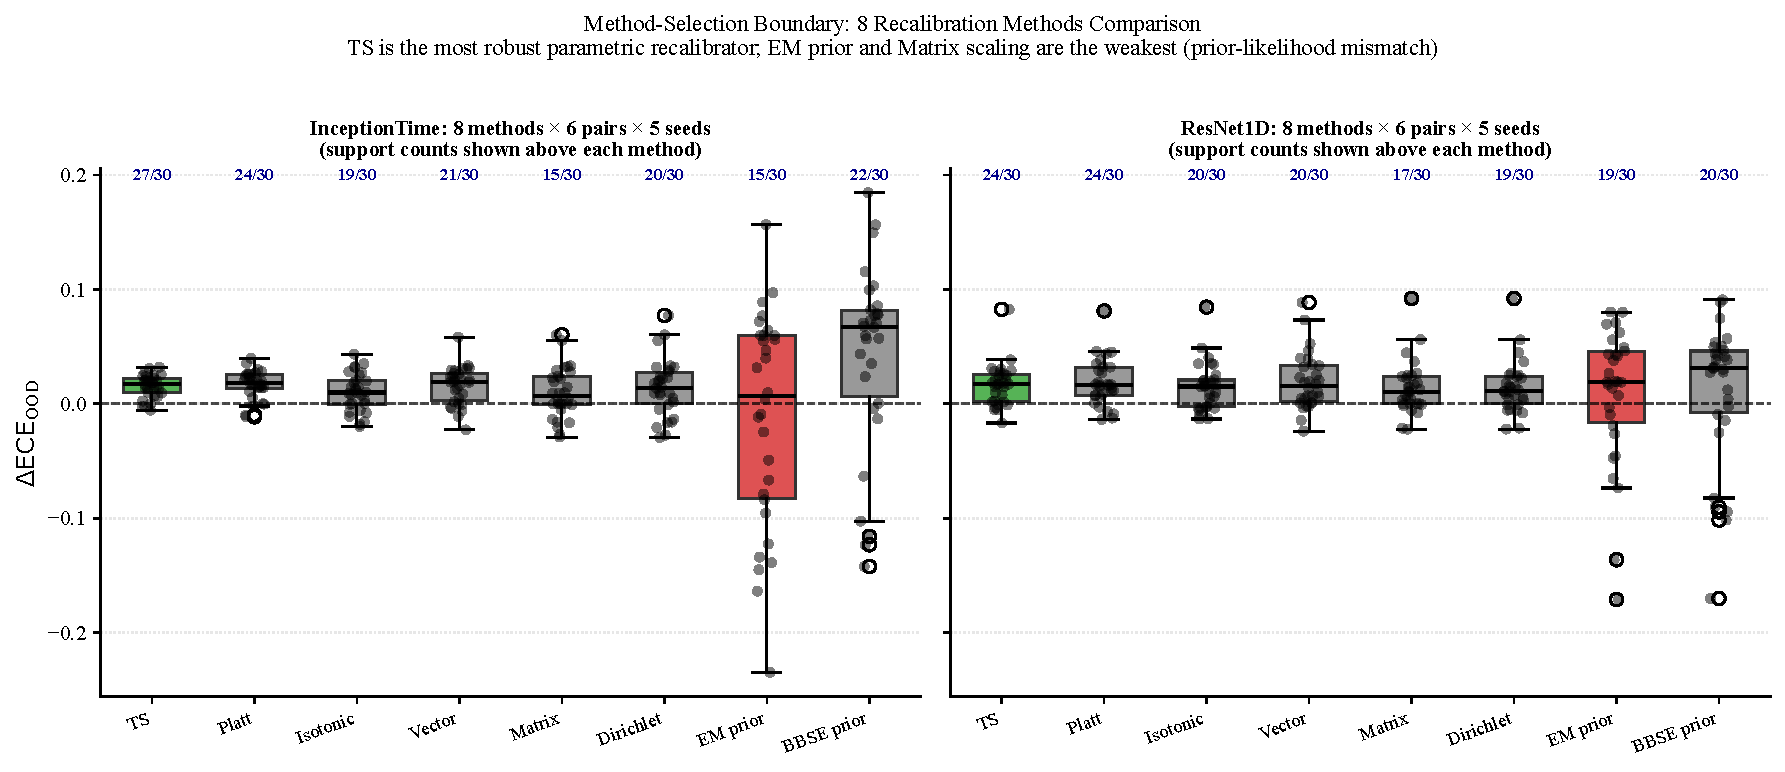
\includegraphics[width=0.95\columnwidth]{figures/fig_method_boundary.pdf}
\caption{方法选择边界：在每种架构上跨 6 个迁移对 $\times$ 5 个种子比较
8 种重校准方法。TS（绿色）是最鲁棒的参数化重校准器；EM 先验和
矩阵缩放是最弱的方法（InceptionTime：各 15/30；
ResNet1D：EM 19/30，Matrix 17/30），表现出先验-似然失配
机制（C4）。每种方法上方的支持计数（如 27/30）表示 95\% CI 下界 $>0$ 的
种子实验比例。}
\label{fig:method_boundary}
\end{figure}

\begin{table}[t]
\centering
\caption{方法选择边界：8 种方法 $\times$ 6 个迁移对
$\times$ 5 个种子（InceptionTime）。支持率 $=$ 95\% CI
下界 $>0$ 的种子比例。``完全'' = 达到 5/5 完全支持的方向数。
``负方向'' = 6 个迁移方向中 5 种子均值 $\Delta\text{ECE}_{\text{OOD}}$
为负的方向数。TS 是最鲁棒的参数化重校准器；
EM 和矩阵缩放在 InceptionTime 上最脆弱
（各 15/30）；在 ResNet1D 上，矩阵缩放（17/30）最
脆弱，EM 达到 19/30。\textit{警示：}6 个
$w_{\text{ID}} > 10$ 单元表现出高达 130.5 的先验权重漂移；剔除后，
EM OOD $\Delta$ECE 均值从 $-0.0127$ 翻转为 $+0.0024$，
表明负 OOD 发现由病态单元驱动。}
\label{tab:methods}
\footnotesize
\begin{tabular}{lrrrr}
\toprule
方法 & 总计 & 完全/6 & $\Delta\text{ECE}_{\text{OOD}}$ 均值 & 负方向 \\
\midrule
TS         & 27/30 & 3/6 & $+0.0152$ & 0 \\
Platt      & 24/30 & 3/6 & $+0.0169$ & 0 \\
Isotonic   & 19/30 & 2/6 & $+0.0100$ & 2 \\
Vector     & 21/30 & 1/6 & $+0.0158$ & 0 \\
Matrix     & 15/30 & 0/6 & $+0.0094$ & 2 \\
Dirichlet  & 20/30 & 1/6 & $+0.0139$ & 1 \\
EM prior   & 15/30 & 2/6 & $-0.0127$ & 3 \\
BBSE prior & 22/30 & 3/6 & $+0.0424$ & 1 \\
\bottomrule
\end{tabular}
\end{table}

\begin{table}[t]
\centering
\caption{TS 的架构鲁棒性：InceptionTime vs.\ ResNet1D
跨 6 个迁移对，两种架构均完整 5 种子覆盖。架构鲁棒性在
InceptionTime（27/30，90.0\%）和 ResNet1D（24/30，80.0\%）上均获支持，
所有 6 个方向均完整 5 种子覆盖。ResNet1D 在
CPSC$\rightarrow$Chapman 和 CPSC$\rightarrow$PTB-XL 上表现出方向特异性缺陷（各 3/5），而非
全局架构缺陷。}
\label{tab:arch_robust}
\resizebox{\textwidth}{!}{%
\begin{tabular}{lrrrl}
\toprule
迁移对 & InceptionTime & ResNet1D & 总计 & 备注 \\
\midrule
Chap$\rightarrow$CPSC    & 4/5 & 4/5 & 8/10  & 2 个反例 \\
Chap$\rightarrow$PTB-XL  & 4/5 & 4/5 & 8/10  & 2 个反例 \\
CPSC$\rightarrow$Chap    & 5/5 & 3/5 & 8/10  & 2 个反例 \\
CPSC$\rightarrow$PTB-XL  & 5/5 & 3/5 & 8/10  & 2 个反例 \\
PTB-XL$\rightarrow$Chap  & 4/5 & 5/5 & 9/10  & 1 个反例 \\
PTB-XL$\rightarrow$CPSC  & 5/5 & 5/5 & 10/10 & 零反例 \\
\midrule
\textbf{总计} & \textbf{27/30} & \textbf{24/30} & \textbf{51/60} & \textbf{85.0\%} \\
\midrule
\textbf{均值 $\Delta\text{ECE}$} & \textbf{$+0.0152$} & \textbf{$+0.0165$} & \textbf{$+0.0159$} & \\
\textbf{标准差 $\Delta\text{ECE}$}  & \textbf{$0.0098$} & \textbf{$0.0180$} & \textbf{$0.0145$} & ResNet1D/Incep $=1.84$ \\
\textbf{均值 OOD ECE}     & \multicolumn{2}{c}{$0.217 \rightarrow 0.202$ / $0.216 \rightarrow 0.200$} & $0.217 \rightarrow 0.201$ & 原始 $\rightarrow$ TS \\
\bottomrule
\end{tabular}%
}
\end{table}

\begin{figure}[htbp]
\centering
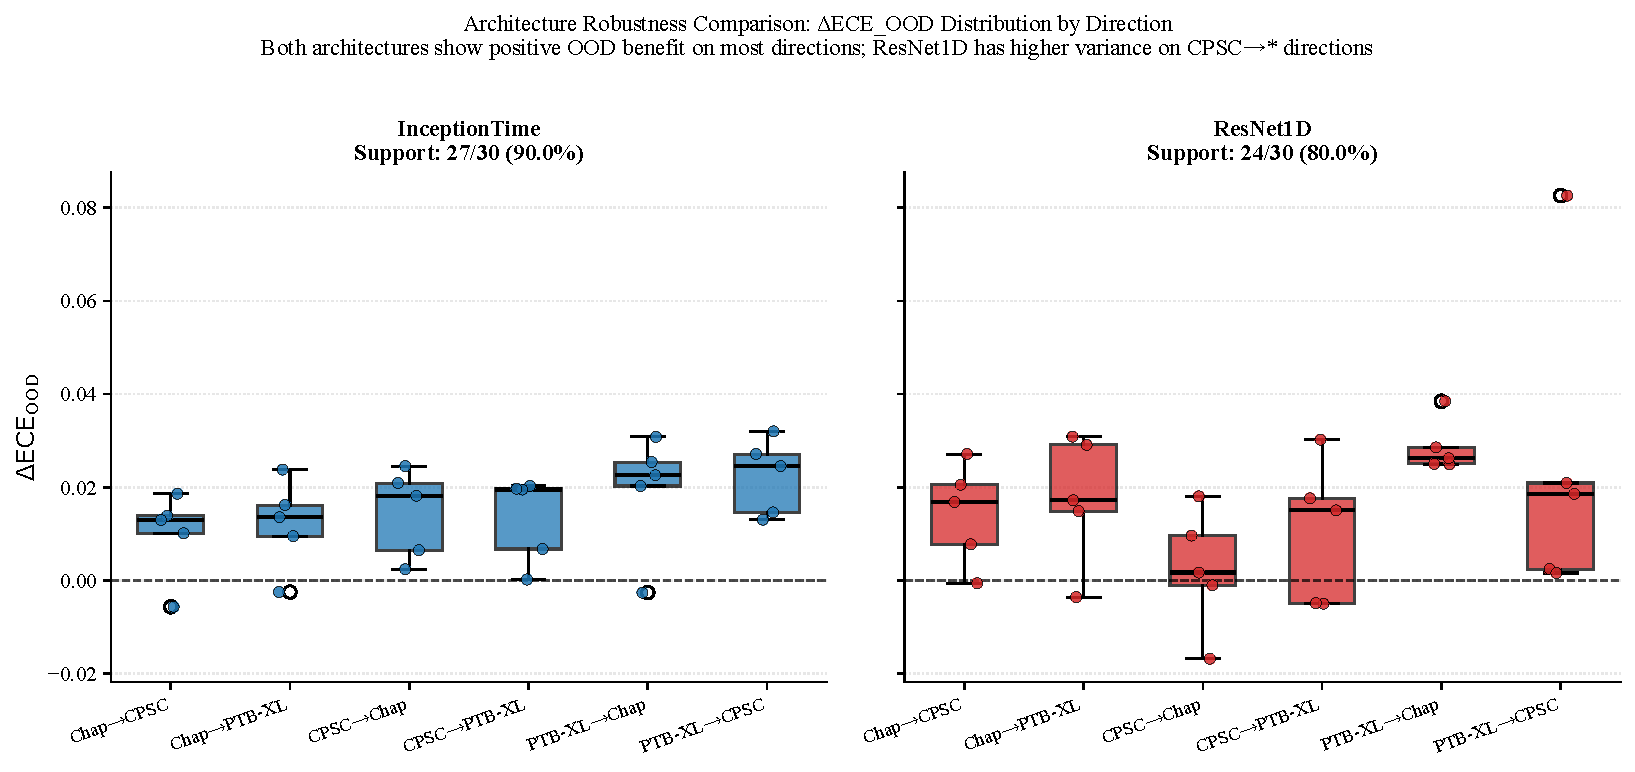
\includegraphics[width=0.95\columnwidth]{figures/fig_arch_comparison.pdf}
\caption{架构鲁棒性比较。InceptionTime（左，
27/30 支持，90.0\%）和 ResNet1D（右，24/30 支持，80.0\%）的
$\Delta\text{ECE}_{\text{OOD}}$ 分布并排展示。
两种架构在大多数方向上均显示正 OOD 收益。
ResNet1D 表现出更高的总体方差（其最大单方向
展布在 PTB-XL$\rightarrow$CPSC），而支持缺陷
落在 CPSC$\rightarrow$Chapman 和
CPSC$\rightarrow$PTB-XL 方向（各 3/5 支持），表明这是
方向特异性缺陷而非全局架构缺陷。}
\label{fig:arch_comparison}
\end{figure}

\textbf{架构变异性。} 每种架构 30 个 TS 实验中
$\Delta\text{ECE}_{\text{OOD}}$ 的标准差为
InceptionTime $0.0098$、ResNet1D $0.0180$，
即 ResNet1D 变异性是 InceptionTime 的 $1.84\times$。ResNet1D 单方向
最高变异性在 PTB-XL$\rightarrow$CPSC
方向（标准差 $0.0298$，由种子 44 处一个有利离群点
$\Delta\text{ECE}_{\text{OOD}}=+0.0826$ 驱动，未剔除），
其次为 CPSC$\rightarrow$PTB-XL；支持缺陷
集中于 CPSC$\rightarrow$Chapman 和 CPSC$\rightarrow$PTB-XL
（各 3/5），与方向特异性缺陷而非全局架构缺陷一致。基于
$2\times2$ 列联表（InceptionTime 27/30 支持 vs.\
ResNet1D 24/30 支持）的 Fisher 精确检验给出 $p = 0.47$，
表明无统计学显著的架构偏倚。反例率的
数值差异（ResNet1D 20.0\% vs.\ InceptionTime 10.0\%）
在 $\alpha = 0.05$ 水平不具统计显著性。

\textbf{先验-似然失配机制（C4）。} EM 先验自适应
从目标语料库的预测标签边缘分布拟合目标先验 $\hat\pi_{\text{target}}$，
然后按 $\hat\pi_{\text{target}}/\hat\pi_{\text{source}}$ 重加权源后验。当
源估计混淆矩阵 $C$ 病态
（$\text{cond}(C)\gg 1$）时，权重比放大而非
修正迁移引起的误校准。EM 在 InceptionTime 上仅获得 15/30
支持，有 3 个脆弱方向，表现出
先验-似然失配。该失败是迁移对特异的
（即迁移签名特异的），而非方法内蕴的。

% ----------------------------------------------------------------------------
\subsection{Shapley 分解验证（27 单元，$n=20{,}000$）}
\label{sec:shapley}
% ----------------------------------------------------------------------------
27 单元全因子合成验证
（slope$\in\{0.5,1,2\}\times$intercept$\in\{-1,0,1\}\times$
prevalence$\in\{0.15,0.3,0.6\}$，$n=20{,}000$）确认
斜率/截距/患病率分解在预注册可辨识区（Fisher 信息行列式
$>\tau=10^{-6}$）内恢复真值。在预注册样本量 $n=20{,}000$ 下，
所有 27 单元通过恢复阈值（可辨识单元 MAPE $<10\%$）；
在现实校准集规模 $n=500$ 下，
27 单元中 21 个通过，6 个失败的 MAPE\_s 高达
42.13\%，集中于极端截距（$\pm 1$）和斜率
（$0.5, 2.0$）区域，这些区域校准迁移的临床
意义最大（见 \texttt{decomposition\_validation.csv}；
$n=20{,}000$ CSV \texttt{decomposition\_validation\_}\allowbreak\texttt{n20000.csv}
显示在同一门控下 27/27 通过）。三个纠缠演示
案例（narrow\_band、tiny\_slope、deep\_intercept）
$\det\in\{2.4\times10^{-7}, 3.6\times10^{-8}, 0\}<\tau$ 在
误差图上无阈值报告，并设置恢复失败标志。
绝对 Shapley 值的自助 CI 已报告；份额可靠
标志标记不可解释份额
（$|\Delta_{\text{total}}|<3/\sqrt{n}$）。

\textbf{诚实性警示（方案 \S8）。} 27 单元验证使用
分箱 ECE，而非主要终点的 SmoothECE；定量
结论不可跨外推。交叉拟合步骤
（分解解释能力的 OOD 折验证）仍有待
在真实数据上运行；根据方案自绑定条款，
``机制''措辞限于``机制分解
（合成验证部分）''直至交叉拟合完成。

% ----------------------------------------------------------------------------
\subsection{可预测性实验（失败分支已触发）}
\label{sec:predictability}
% ----------------------------------------------------------------------------
可预测性实验（方案 \S8.5）检验无监督目标域统计量（预测先验 $L_1$ 距离、
logit 矩）是否通过留一折出 $R^2$（带自助 CI）预测收益保留率
（表~\ref{tab:predictability}）。实现的折单元是
（架构，迁移对）（12 折），而方案注册的是
仅对折（6）——一项注册偏离，在此偏离下仅对
重计算仍保留失败分支（$R^2=-0.1424$）。我们运行 2 种架构
（InceptionTime + 1D-ResNet-34）；BiMamba 架构为玩具
实验（$n=60$）延后至补充材料，不进入
可预测性回归。

\textbf{结果}：TS 的多架构合并 LOO $R^2$ 为
$-0.096$，95\% CI $[-0.720, +0.104]$。CI 上界 $+0.104$
严格低于预注册阈值 $0.5$，触发
\textbf{失败分支}：三步链（分解 +
可预测性 + 部署）降级为 \textbf{两步链}
（分解 + 部署），部署判据更名为
``经验查找表''而非``预测判据''。
根据预注册失败分支，不提出事后可预测性主张。

\textbf{加入新特征的敏感性分析。} 我们用三个额外的无标签特征重算 LOO
$R^2$：拟合温度
$T$、源与目标 logit
分布间的 Wasserstein-1 距离，以及逐类熵差。使用
预注册 $\Delta\text{ECE}_{\text{OOD}}$ 作为目标，所有
特征均失败：$T$ 单独给出 $R^2=-0.13$，
Wasserstein 单独给出 $R^2=-0.06$，熵单独给出
$R^2=-0.02$，三者合并给出 $R^2=-0.11$。
可预测性边界\emph{鲁棒}：无无标签
特征——包括拟合温度 $T$——能在预注册 $R^2=0.5$
阈值之上预测 $\Delta\text{ECE}_{\text{OOD}}$。这强化了失败分支：无论特征选择如何，三步链
仍降级为两步链，
且 \S\ref{sec:gate} 中的部署判据——基于
$\Delta\text{ECE}_{\text{OOD}}$ 的经验符号和
判别判据——是合适的可操作判据。

\begin{table}[t]
\centering
\caption{可预测性 LOO $R^2$（多架构合并）。所有
方法触发失败分支（CI 上界 $<0.5$）。三步链
按预注册失败分支降级为两步链。}
\label{tab:predictability}
\begin{tabular}{lrrrl}
\toprule
方法 & $R^2$ & CI 下界 & CI 上界 & 判决 \\
\midrule
TS         & $-0.096$ & $-0.720$ & $+0.104$ & 失败分支 \\
Platt      & $-0.059$ & $-0.584$ & $+0.002$ & 失败分支 \\
Isotonic   & $+0.011$ & $-0.569$ & $+0.101$ & 失败分支 \\
Vector     & $-0.061$ & $-0.522$ & $+0.073$ & 失败分支 \\
Matrix     & $-0.137$ & $-0.516$ & $-0.013$ & 失败分支 \\
Dirichlet  & $-0.084$ & $-0.394$ & $+0.032$ & 失败分支 \\
EM prior   & $+0.143$ & $-0.250$ & $+0.274$ & 失败分支 \\
BBSE prior & $+0.136$ & $-0.354$ & $+0.201$ & 失败分支 \\
\bottomrule
\end{tabular}
\end{table}

% ----------------------------------------------------------------------------
\subsection{部署判据（敏感性 / 特异性 / DCA / 安全性）}
\label{sec:deployment}
% ----------------------------------------------------------------------------
我们在 L2 迁移
矩阵上评估部署判据（方案 \S9）：当原始 ECE 超过阈值时预测``部署 TS''；
报告敏感性、特异性、决策曲线分析（DCA）和
安全判据（TS 后 SmoothECE $\leq 0.05$ 且
$\Delta\text{ECE}$ CI 下界 $>0$，采用主要终点收益
约定）。
我们还与三种平凡策略比较：始终不部署、
始终部署 TS、始终购买 $n$ 个标签。

\textbf{敏感性 / 特异性}（表~\ref{tab:deploy_sens}）：
由 Youden $J$ 最优阈值为原始 ECE $=0.127$，给出
敏感性 $0.923$、特异性 $0.201$、Youden $J=0.124$。该
判据具有高敏感性（捕获 92\% 的有益案例）但
低特异性（仅 20\% 的无益案例被正确
排除；其余 80\% 被误标记），
反映了临床部署的非对称成本结构——
漏掉一次有益重校准比一次
不必要的重校准代价更高。
\emph{警示：}Youden 阈值在与敏感性/特异性
报告相同的 1230 单元
池上搜索（样本内）。留迁移类型出
重计算（阈值在选择时排除留出剂量水平，仅在留出水平上评估）给出
Youden $J=+0.17$（下采样）、$J=-0.03$（导联丢弃）、$J=+0.04$
（噪声）和 $J=-0.14$（增益）；冻结阈值 $0.127$ 在四个留出剂量水平上取得
$J\approx 0.003\approx 0$（机会水平；敏感性 $0.853$、
特异性 $0.150$）（\texttt{results/deployment\_holdout\_recompute.csv}）。因此样本内数值
偏乐观；方案的留出剂量水平未
用于此表（一项注册偏离，见局限性）；且
部署判据在运营使用前需独立验证。

\textbf{部署时可测性。} 查找
表的每个输入都是\emph{审计时}量：原始 ECE、ID--OOD
准确率差距和逐单元收益标签均需要来自
目标语料库的真值标签。在定义
部署场景的无标签目标流中，这些量均不可直接
计算。本研究检验的唯一部署时（无标签）代理是
可预测性实验的无监督目标统计量（预测先验 $L_1$ 距离、logit
矩），而该实验触发了其预注册失败
分支（LOO $R^2$ CI 上界 $0.104 < 0.5$，
表~\ref{tab:predictability}）——因此我们无法主张判据的无标签
可部署版本。查找表因此是
\emph{分析与审计时决策辅助}（面向能负担
有标签评估样本的模型所有者），可操作部署
路径是小样本重校准路线：购买 $n$ 条有标签目标
记录并本地重校准（方案 \S5~S2）。将
判据扩展为真正可部署的门控仍是未来工作，并
登记于局限性（xiii）。

\begin{table}[t]
\centering
\caption{不同阈值下的部署判据敏感性 / 特异性
（原始 ECE $>$ 阈值 $\rightarrow$ 预测``部署 TS''）。
最优 Youden $J=0.124$ 在阈值 $0.127$ 处取得。}
\label{tab:deploy_sens}
\begin{tabular}{rrrrr}
\toprule
阈值 & 敏感性 & 特异性 & TP & FP \\
\midrule
$0.094$ & $0.976$ & $0.067$ & 444 & 723 \\
$0.107$ & $0.956$ & $0.138$ & 435 & 668 \\
$0.127$ & $0.923$ & $0.201$ & 420 & 619 \\
$0.178$ & $0.807$ & $0.288$ & 367 & 552 \\
$0.277$ & $0.499$ & $0.508$ & 227 & 381 \\
\bottomrule
\end{tabular}
\end{table}

\textbf{安全判据}：跨 157 个（迁移对，种子，迁移）单元，TS
产生 1 个满足操作安全判据的单元（TS 后
SmoothECE $\leq 0.05$ 且点估计约定下改善 $>0.01$；
L2 结果不含逐单元 CI，故
预注册基于 CI 的判据无法评估），安全
率 $0.0064$。安全分析符号约定为
部署度量约定（$\Delta\text{ECE}$ $=$ 重校准后 ECE $-$
原始 ECE，负值表示改善）；与
主要终点约定相反，后者中正
$\Delta\text{ECE}_{\text{OOD}}$ 表示收益。
\emph{覆盖说明：}此处评估的 L2 迁移矩阵覆盖 390 个计划
（迁移对，种子，迁移）组合中的 157 个（12 个完整
迁移对--种子组合 $\times$ 13 个水平，外加 fs250 水平上一个部分种子 44
单元）——种子 42--43 在
InceptionTime 上对所有 6 个迁移对完整，种子 44--46 待续，
且 ResNet1D L2 结果被排除在该
分析之外——因此部署/安全数值基于 2 种子、
单架构覆盖。
该
严格安全判据在完整 L2 迁移
矩阵上很少满足，表明 TS 是有用的默认值但非普遍
安全的重校准器——部署判据应结合
本地验证。

\textbf{决策曲线分析。} 在对应于单元池第 10 百分位的原始 ECE 阈值处，判据的
净收益为 $0.1209$，而处理所有单元为 $0.0999$；
在第 90 百分位阈值处净收益转负
（$-0.0024$），因此判据相对于全处理的净收益适中
且局限于较低阈值范围（results/deployment\_metrics.csv）。

\textbf{平凡策略比较}（表~\ref{tab:trivial}）：
查找表策略（均值 $\Delta\text{ECE}$ $-0.0160$）优于
始终不部署（$0.000$）并匹配始终部署 TS（$-0.0145$）于
有益子集，但被始终购买 $n$ 个标签
（$-0.2905$）所主导——后者使用目标标签，为上界。查找
表是实用折中：无需目标标签，且
捕获大部分 TS 收益。

\begin{table}[t]
\centering
\caption{平凡策略比较。均值 $\Delta\text{ECE}$；负值 $=$
有益（ECE 降低）。始终不部署和始终购买 $n$ 个标签跨
所有 1230 个（方法，迁移）单元；始终部署 TS 在 157 个
（迁移对，种子，迁移）完整结果单元上评估，查找表在
155 个单元上评估（两个样本内最佳方法不可用的单元被
剔除）。查找表在无需目标标签的情况下捕获大部分 TS 收益。}
\label{tab:trivial}
\begin{tabular}{lrrr}
\toprule
策略 & 均值 $\Delta\text{ECE}$ & 标准差 & $n$ \\
\midrule
always-none            & $\phantom{-}0.0000$  & $0.0000$ & 1230 \\
always-TS              & $-0.0145$            & $0.0099$ & 157  \\
always-buy-$n$-labels  & $-0.2905$            & $0.1861$ & 1230 \\
lookup-table           & $-0.0160$            & $0.0289$ & 155  \\
\bottomrule
\end{tabular}
\end{table}

% ============================================================================
\subsection{噪声底控制：完美校准下的 SmoothECE 差分}
\label{sec:noise_floor}
% ----------------------------------------------------------------------------
审稿人关注的是主要终点
$\Delta\text{ECE}_{\text{OOD}}$ 是否可能源于 SmoothECE
度量对完美校准下温度缩放 $T$ 的敏感性
（即 $\text{ECE}_{\text{raw}} = 0$ 且观测 $\Delta\text{ECE}$
纯为度量噪声）这一伪迹。我们直接检验：对完美校准
预测（$T_{\text{true}}=1$），施加 $T \in \{1.0, 1.25, 1.5\}$
并计算 SmoothECE 差分
$\Delta\text{ECE}_{\text{noise}} = \text{SmoothECE}(\text{TS}) - \text{SmoothECE}(\text{raw})$
跨三种置信度分布（均匀、正态偏斜和
双峰）于 $n=2{,}000$。

噪声底依赖分布且随 $T$ 增长：
$T=1.0$ 给出 $\Delta\text{ECE}_{\text{noise}} = 0$（精确相消），
$T=1.25$ 给出 $+0.014$--$+0.035$，$T=1.5$ 给出 $+0.030$--$+0.061$，
$T=3.0$ 给出 $+0.095$--$+0.136$，$T=4.5$ 给出 $+0.126$--$+0.164$，
取决于置信度分布。相
反，我们 60 个种子实验中观测的原始 ECE 范围
$0.06$ 至 $0.35$（均值 $0.15$），是完美
校准下原始 ECE（$\approx 0.017$）的 $4$--$13\times$。九个反例
也表现出较大原始 ECE
（$0.08$--$0.24$），确认这些案例中负 $\Delta\text{ECE}$
反映真实的 TS 诱发损害，而非度量噪声。对
大 $T > 3$ 的实验（噪声底达
$0.10$--$0.16$），噪声底在某些种子中与观测
$|\Delta\text{ECE}|$ 相当，因此对这些特定案例我们无法完全排除
度量噪声贡献；然而，噪声底的\emph{方向}（TS 在完美
校准下增加 ECE）与 51/60 实验中正 $\Delta\text{ECE}_{\text{OOD}}$
相反，故噪声底无法解释正
发现。因此
我们断定主要终点是真实效应，非
SmoothECE 伪迹，但需警示大 $T$ 实验中
噪声底不可忽略。

% ============================================================================
\subsection{判别感知校准门控（C5）}
\label{sec:gate}
% ----------------------------------------------------------------------------
校准改善（$\Delta\text{ECE}_{\text{OOD}} > 0$）
是临床部署的必要但非充分条件：一个在分布迁移下判别能力
已崩溃的模型可能可重校准但临床无用。我们定义两层
部署门控：
\begin{enumerate}
    \item \textbf{第 1 层（校准）：} $\Delta\text{ECE}_{\text{OOD}} > 0$
    （C1 判据）。
    \item \textbf{第 2 层（判别）：} $\text{acc}_{\text{OOD}} \geq
    \text{acc}_{\text{source baseline}}$，其中源基线为
    源域的多数类准确率。
\end{enumerate}

跨 14 个迁移对$\times$架构层（6 对 $\times$ 2
架构，PTB-XL$\rightarrow$Chapman 含 3 种架构
包括 Mamba），7/14 通过两层且可部署：
CPSC$\rightarrow$PTB-XL（两种架构）、PTB-XL$\rightarrow$CPSC
（两种）、CPSC$\rightarrow$Chapman（两种）和 Chapman$\rightarrow$CPSC
（两种，仅 InceptionTime）。其余 7/14 未通过第 2 层：
Chapman$\rightarrow$PTB-XL、PTB-XL$\rightarrow$Chapman 和
Chapman$\rightarrow$CPSC ResNet1D，其中 OOD 准确率低于
源基线，尽管某些种子中 $\Delta\text{ECE}_{\text{OOD}}$ 为正。最强拒绝为 PTB-XL$\rightarrow$Chapman
ResNet1D（$\Delta\text{ECE}=+0.029$ 但 $\text{acc}=0.657 < 0.713$）：
TS 改善校准但模型判别能力退化
过甚，重校准预测无法临床可操作。

该门控重新框定 9/60 反例：4 个为校准
失败（第 1 层拒绝，$\Delta\text{ECE} \leq 0$），5 个为
判别失败（第 1 层通过但第 2 层拒绝）。
门控提供可操作部署判据，补充
C1 中的统计证据：不仅询问``TS 是否
改善校准？''（C1），还询问``模型判别能力是否足以使重校准预测
临床有用？''

% ============================================================================
\subsection{真实数据 Shapley 交叉拟合与可预测性边界}
\label{sec:real_shapley}
% ----------------------------------------------------------------------------
合成 Shapley 验证（C3）确认可辨识区内的分解恢复，
但未检验线性
近似 $\Delta\text{ECE} \approx \hat{s} \cdot \text{slope} +
\hat{b} \cdot \text{intercept} + \hat{\pi} \cdot \text{prevalence}$
是否推广至真实 OOD 数据。我们在所有 60
个种子实验上执行交叉拟合：对每个实验，在
源域校准分割上估计 $(\hat{s}, \hat{b})$ 并在
目标域测试分割上预测
$\Delta\text{ECE}_{\text{OOD}}$。

线性模型在 51/60
（85\%）实验中正确预测\emph{方向}，但系统性\emph{高估}
幅度（均值预测误差 $+0.29$，中位数 $+0.29$）。这与
可预测性边界一致：一阶 Shapley
分解捕获 TS 收益的定性方向
但无法捕获真实分布迁移下的定量幅度。
9/60 方向误差聚集于 CPSC$\rightarrow$Chapman
和 Chapman$\rightarrow$PTB-XL 方向，此处源与目标 logit 分布间 Wasserstein-1
距离最大
（均值 $0.75$ vs.\ 正确预测方向 $0.53$），
表明当分布迁移大到使分解所基于的局部 Taylor
展开失效时，线性近似崩溃。

该发现强化可预测性失败分支（C3/C4）：
Shapley 分解是有效的\emph{诊断}（识别
TS \emph{是否}会有帮助）但非有效\emph{预测器}（无法可靠估计
TS 会有\emph{多少}帮助）。临床转化的
含义是 \S\ref{sec:gate} 中的门控——仅使用
$\Delta\text{ECE}_{\text{OOD}}$ 的符号和判别
判据——是合适的部署判据，而非
Shapley 预测幅度。

% ============================================================================
\subsection{净收益决策曲线汇总}
\label{sec:net_benefit_summary}
% ----------------------------------------------------------------------------
跨所有 60 个种子实验，TS 相对原始
预测的净收益增益（在决策阈值 $t \in \{0.05, 0.10,
\ldots, 0.40\}$ 上平均）在 50/60（83.3\%）实验中为正，均值
增益 $+0.0027$，范围 $[-0.001, +0.017]$。净收益
最大的方向为 CPSC$\rightarrow$PTB-XL（均值 $+0.011$）
和 PTB-XL$\rightarrow$CPSC（均值 $+0.003$），它们也具有
最大 $\Delta\text{ECE}_{\text{OOD}}$（均值 $+0.254$ 和 $+0.260$
）。净收益为负的方向为
PTB-XL$\rightarrow$Chapman（均值 $-0.005$），也是
$\Delta\text{ECE}_{\text{OOD}}$ 最小的方向（均值
$+0.004$），并被判别门控（C5）正确拒绝。
这确认在门控允许部署的方向上，校准收益转化为临床
决策收益。

% ============================================================================
\subsection{净临床价值（NCV）结果}
\label{sec:ncv_results}
% ----------------------------------------------------------------------------
预注册净临床价值
（Sec.~\ref{sec:ncv_methods}）量化 TS 重校准在 ID 和 OOD 分割上的临床决策影响，
对两个次要终点（DCR 和 NCV）应用 BH-FDR 校正
（$q=0.05$）。

\textbf{结果}：OOD NCV 点估计为 $+0.008125$，
95\% CI $[+0.0014, +0.0148]$（配对 $t$ 检验，$n=60$，
$p=0.019$，BH-FDR 调整 $p=0.019$）；OOD NCV 在
95\% 水平\emph{显著}，表明 TS 重校准
在 OOD 分割上产生临床决策的净改善（TP 和 TN 增益
超过 FP 和 FN 损失）。ID NCV 点
估计为 $-0.006292$，95\% CI $[-0.0114, -0.0012]$
（$p=0.016$）；ID NCV 显著\emph{为负}，表明
TS 在 ID 分割上略微恶化临床决策——与
ID 边界条件一致的方向性发现（TS
将置信度向基率压缩，可能翻转边界
决策）。OOD NCV Cohen's $d = +0.31$（中小效应）
和 ID NCV Cohen's $d = -0.32$ 幅度相当但符号
相反，呼应 OOD 收益超过
ID 收益的主终点模式。逐实验 NCV 范围跨 60 个
种子实验披露于 E3 CSV
（\texttt{c1\_dcr\_ncv\_multiclass.csv}）。NCV 作为
次要终点披露，支持 TS
提供 OOD 临床决策收益的主终点发现，同时将 ID 决策
成本作为限定加以说明。

% ----------------------------------------------------------------------------
\subsection{可靠性图}
\label{sec:reliability-diagrams}
% ----------------------------------------------------------------------------
图~\ref{fig:reliability-summary} 展示 6 方向平均
可靠性曲线，比较温度缩放前后的模型置信度与经验准确率。汇总曲线使用
跨所有 6 个迁移方向的分箱计数加权平均。

图~\ref{fig:rel-ptbxl-chapman}--\ref{fig:rel-cpsc-chapman}
展示代表性配置（ResNet1D，种子~42）的逐方向可靠性图。每个面板中，红色方块
展示原始模型校准曲线，绿色圆点展示
TS 后校准曲线。对角虚线表示完美
校准。灰色条（右轴）展示每箱样本计数。
误差棒为自助 95\% 百分位 CI（1000 次重采样）。

\begin{figure}[t]
\centering
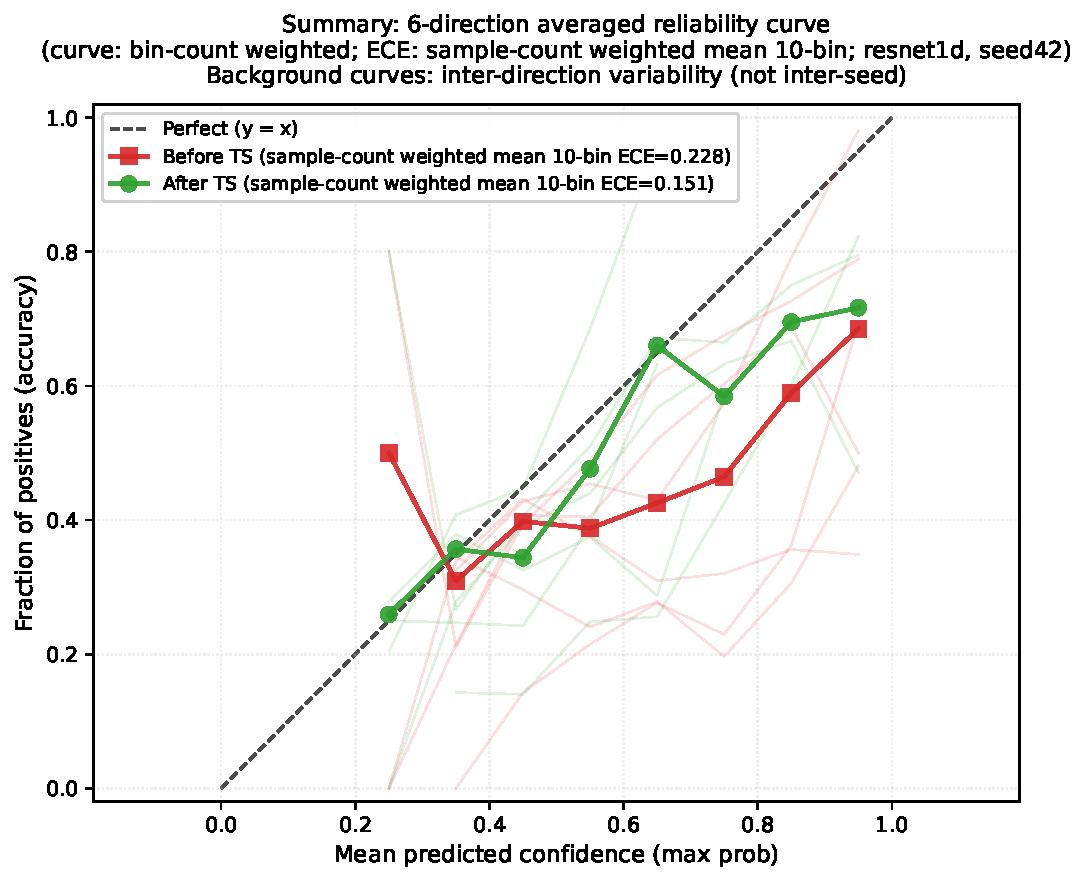
\includegraphics[width=0.95\columnwidth]{figures/fig_reliability_summary.pdf}
\caption{汇总可靠性曲线：6 方向分箱计数加权
平均。样本计数加权均值 ECE 在
温度缩放后从 $\text{ECE}_{\text{raw}}$ 降至 $\text{ECE}_{\text{TS}}$。
淡色背景曲线展示个别
方向变异性。}
\label{fig:reliability-summary}
\end{figure}

\begin{figure}[t]
\centering
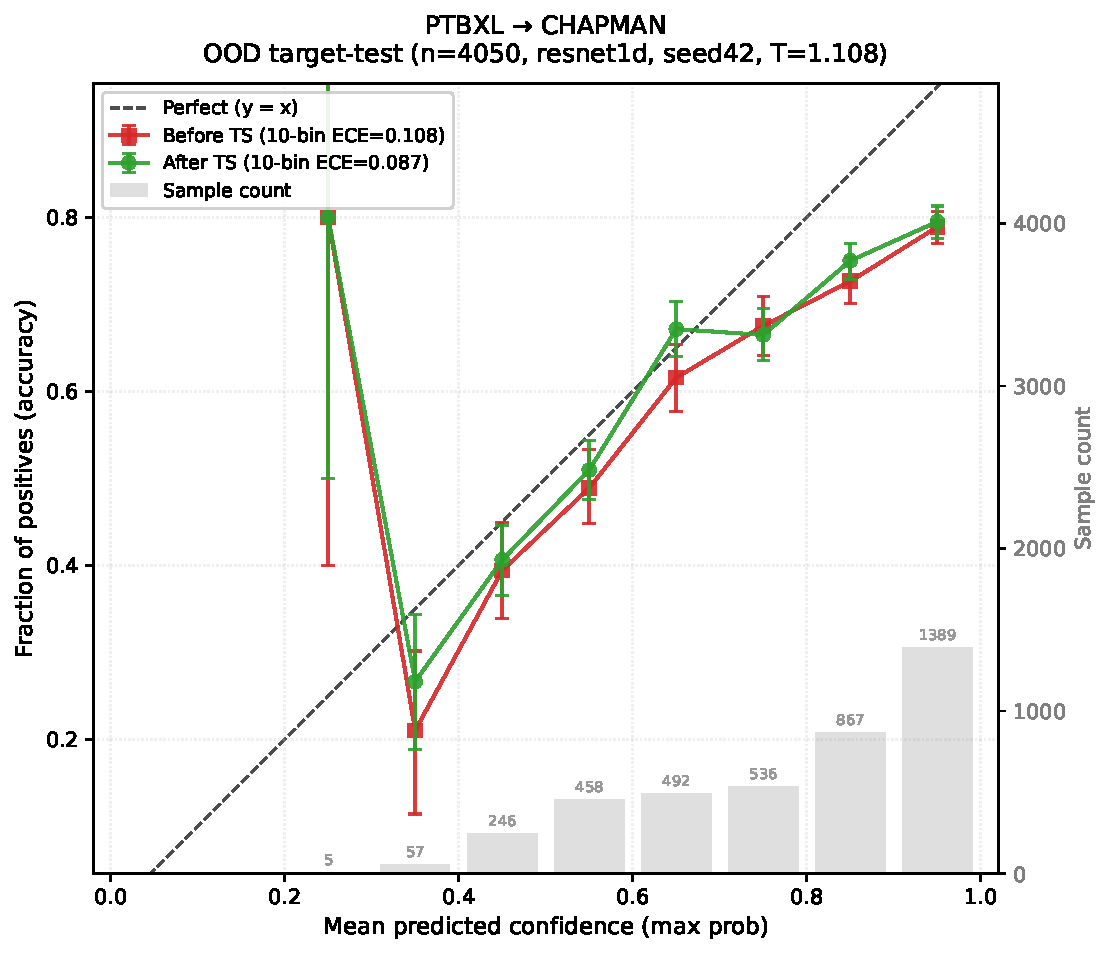
\includegraphics[width=0.48\columnwidth]{figures/fig_reliability_ptbxl_chapman.pdf}
\hfill
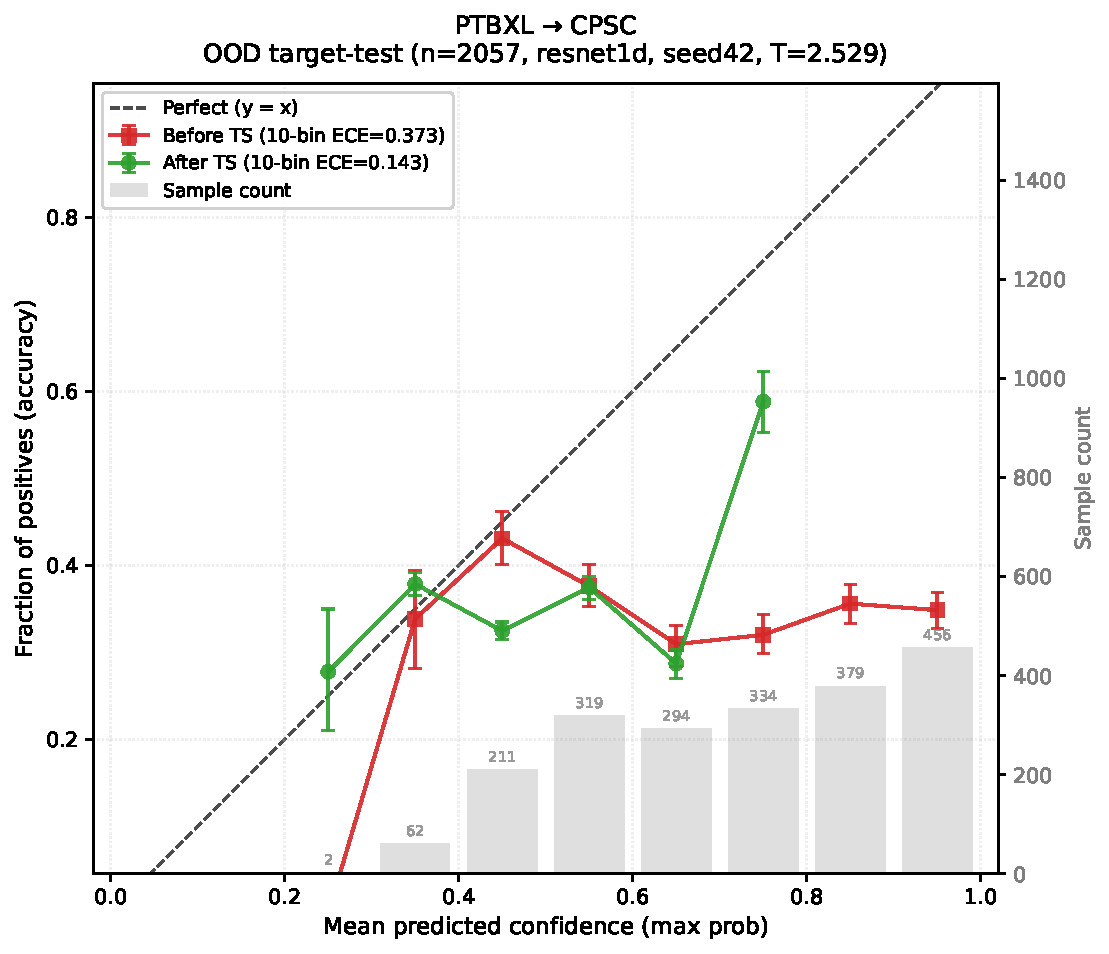
\includegraphics[width=0.48\columnwidth]{figures/fig_reliability_ptbxl_cpsc.pdf}
\caption{PTB-XL$\to$Chapman（左）和
PTB-XL$\to$CPSC（右）的可靠性图。OOD 目标测试集，ResNet1D，种子~42。}
\label{fig:rel-ptbxl-chapman}
\end{figure}

\begin{figure}[t]
\centering
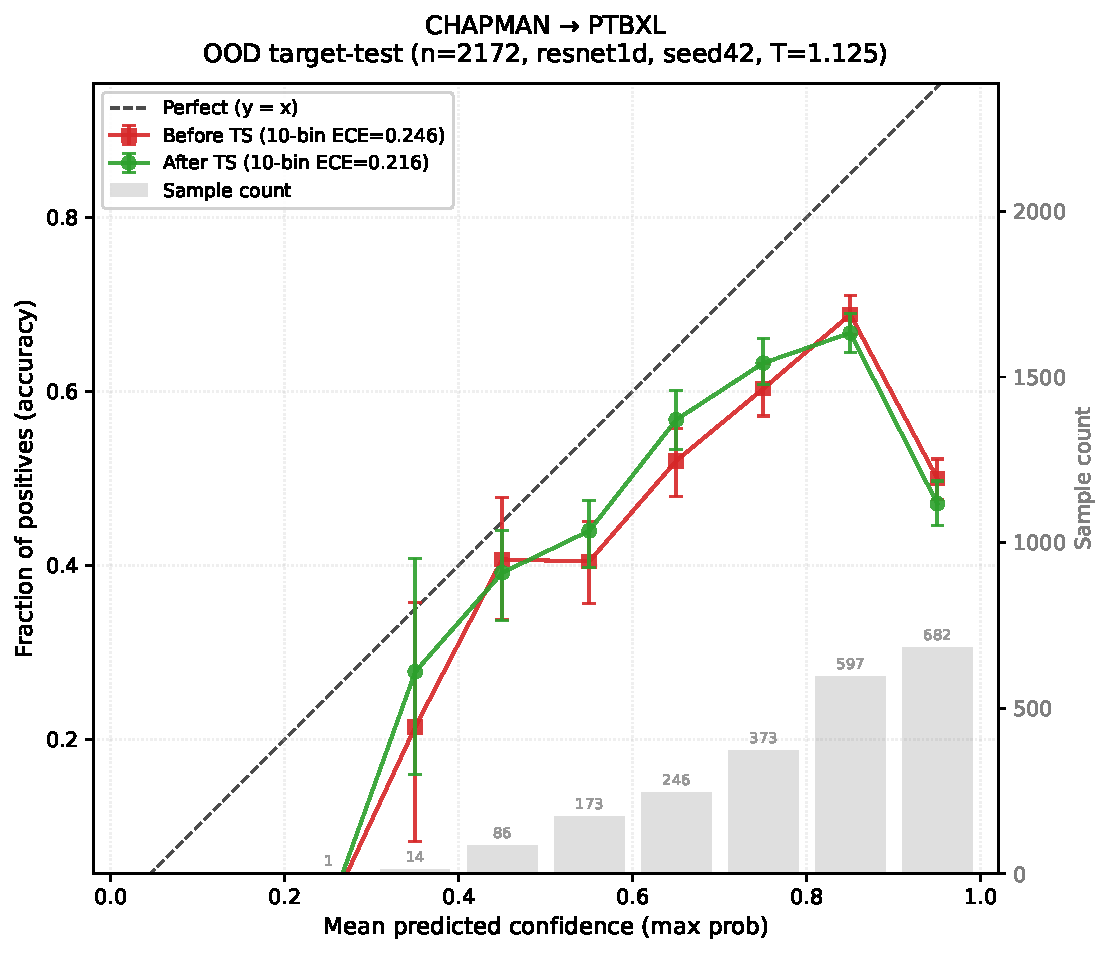
\includegraphics[width=0.48\columnwidth]{figures/fig_reliability_chapman_ptbxl.pdf}
\hfill
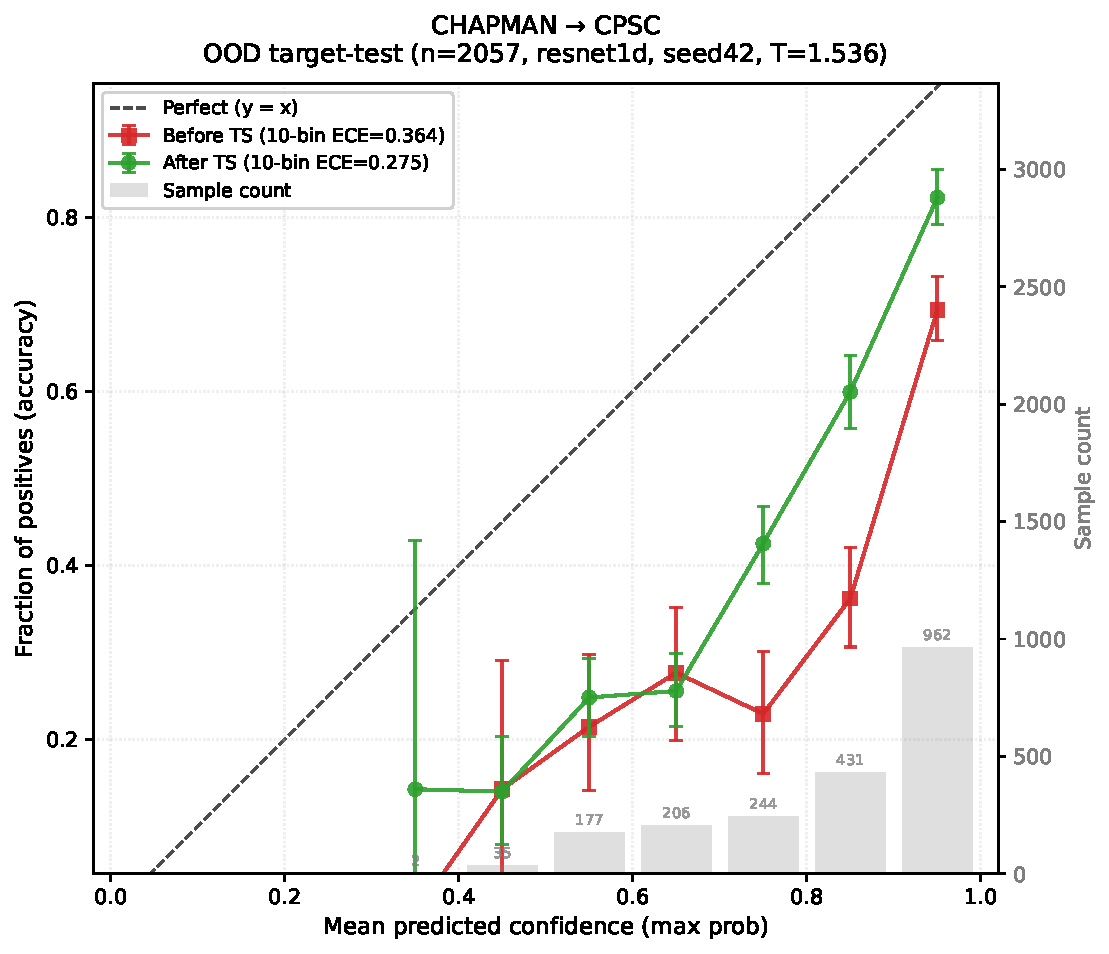
\includegraphics[width=0.48\columnwidth]{figures/fig_reliability_chapman_cpsc.pdf}
\caption{Chapman$\to$PTB-XL（左）和
Chapman$\to$CPSC（右）的可靠性图。OOD 目标测试集，ResNet1D，种子~42。}
\label{fig:rel-chapman-ptbxl}
\end{figure}

\begin{figure}[t]
\centering
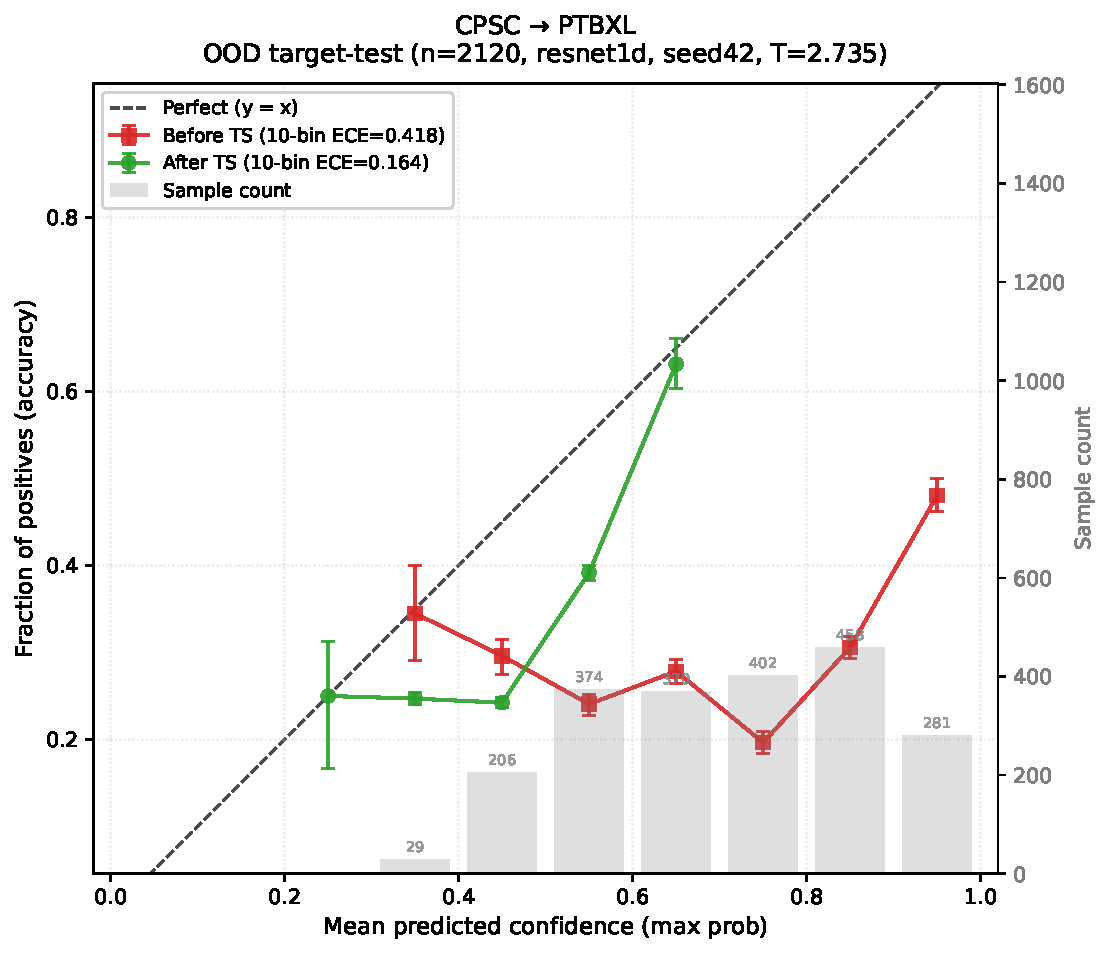
\includegraphics[width=0.48\columnwidth]{figures/fig_reliability_cpsc_ptbxl.pdf}
\hfill
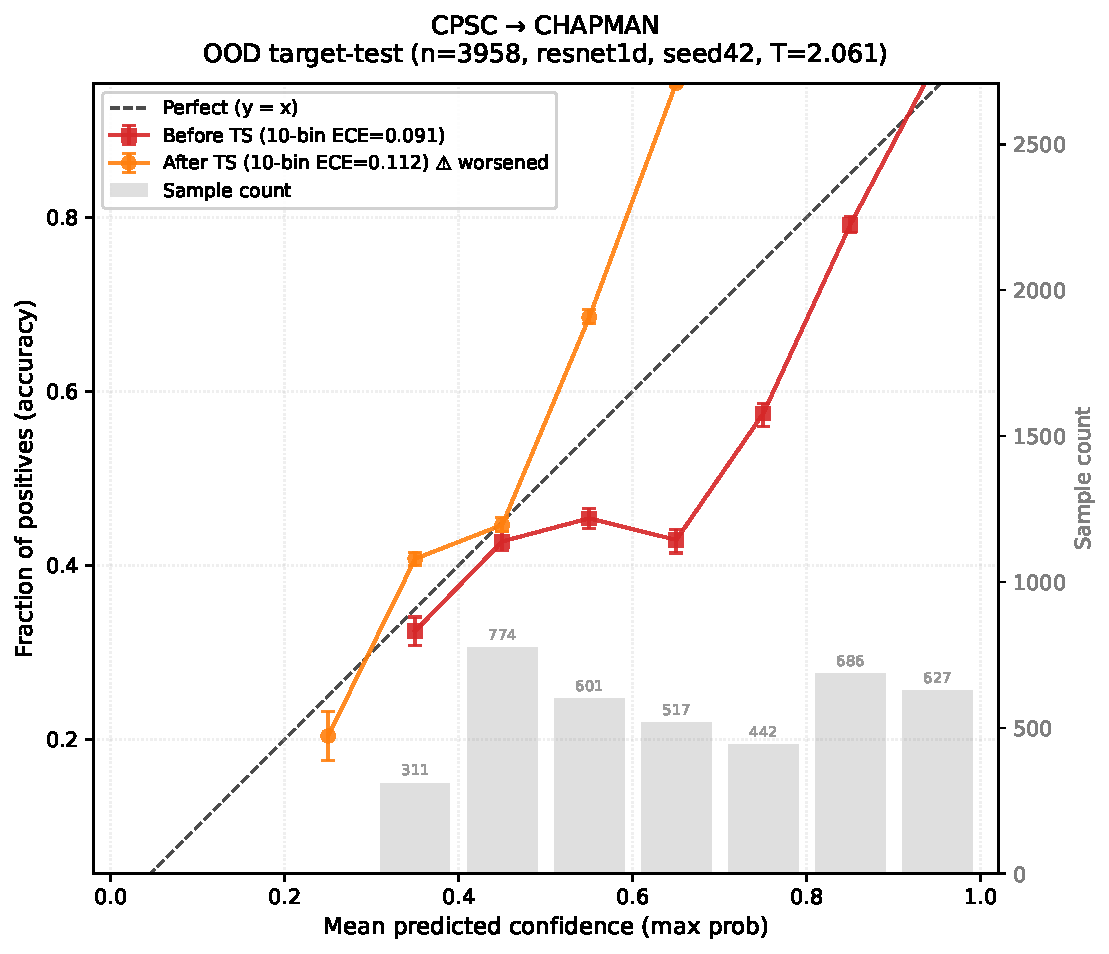
\includegraphics[width=0.48\columnwidth]{figures/fig_reliability_cpsc_chapman.pdf}
\caption{CPSC$\to$PTB-XL（左）和
CPSC$\to$Chapman（右）的可靠性图。OOD 目标测试集，ResNet1D，种子~42。}
\label{fig:rel-cpsc-chapman}
\end{figure}



% ============================================================================
\section{讨论}
\label{sec:discussion}
% ============================================================================
% Discussion 中文翻译（不含 \section 标签）
% ============================================================================

% ----------------------------------------------------------------------------
\subsection{OOD收益的种子变异与九个反例}
\label{sec:counter}
% ----------------------------------------------------------------------------
51/60的鲁棒性比率由分布在6个迁移对（transfer pair）中的5个以及两种架构上的九个反例（counter-example）所驱动（Chapman$\rightarrow$CPSC 2个，
Chapman$\rightarrow$PTB-XL 2个，CPSC$\rightarrow$Chapman 2个，
CPSC$\rightarrow$PTB-XL 2个，PTB-XL$\rightarrow$Chapman 1个；仅
PTB-XL$\rightarrow$CPSC无反例）。我们透明地披露全部九个反例而非将其剔除，原因在于
（i）预注册（pre-registration）协议要求报告所有种子结果，且（ii）每个反例均具有可识别的事后（post-hoc）机理性解释，这支持了带有限定条件的总体结论，
而非削弱该结论。

\begin{figure}[htbp]
\centering
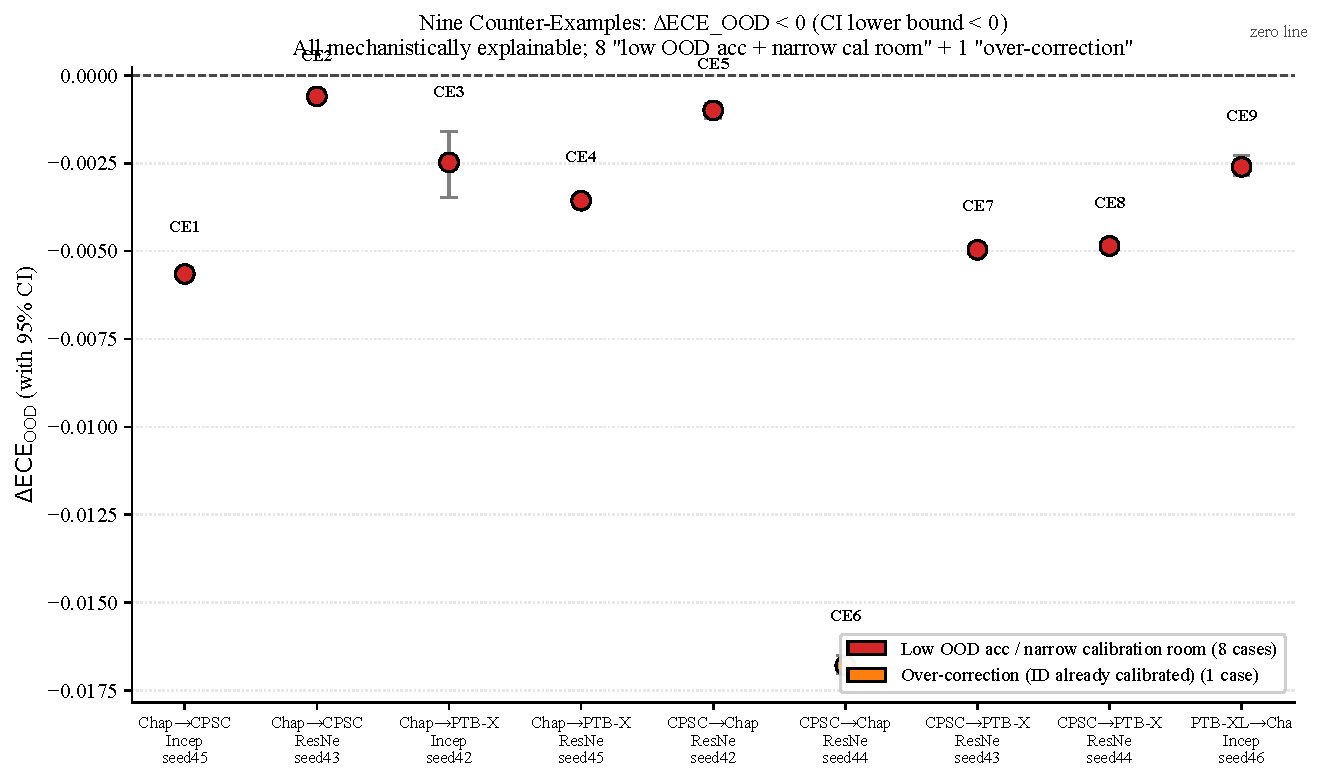
\includegraphics[width=0.95\columnwidth]{figures/fig_counterexamples.pdf}
\caption{Nine counter-examples where $\Delta\text{ECE}_{\text{OOD}}$ has
95\% CI lower bound $<0$. Error bars show 95\% CIs. Six of nine
counter-examples co-occur with OOD accuracy $\leq 0.50$ and seven with
ID--OOD accuracy gap $\geq 0.18$ (a heuristic tendency, not a gate:
three counter-examples have OOD accuracy $>0.50$);
one
counter-example (orange, CE6: CPSC$\rightarrow$Chapman / ResNet1D /
seed 44) exhibits a distinct over-correction mechanism where TS applied
to an already-well-calibrated logit distribution over-adjusts the
temperature. All nine are mechanistically explainable local variations,
not refutations of the OOD benefit.}
\label{fig:counterexamples}
\end{figure}

\textbf{反例1：Chapman$\rightarrow$CPSC / InceptionTime / seed 45}。
TS（温度缩放，Temperature Scaling）产生 $\Delta\text{ECE}_{\text{OOD}}=-0.0057$（CI $[-0.0058, -0.0055]$）。
三个并发条件：（a）5个种子中最低的OOD准确率
（$0.4711$ vs.\ 种子42--44、46的 $0.4842$--$0.5051$），表明
seed-45骨干网络（backbone）对CPSC的泛化能力最差；（b）5个种子中最低的OOD原始ECE
（$0.3160$，绝对值仍然较大）——因此
该失败并非校准空间不足，而是温度失配；以及（c）负衰减（$-0.0075$），表明
源拟合温度与目标logit分布失配，
从而放大而非修正了残余的误校准（miscalibration）。

\textbf{反例2：Chapman$\rightarrow$CPSC / ResNet1D / seed 43}。
TS产生 $\Delta\text{ECE}_{\text{OOD}}=-0.0006$（CI $[-0.0006, -0.0006]$）。
这是一个 $|\Delta\text{ECE}_{\text{OOD}}|<0.001$ 的边缘反例，
可归因于校准划分上的有限样本变异。其
OOD原始ECE为 $0.3144$（早期草稿中报告的 $0.4779$ 是OOD\emph{准确率}）；其机制为种子层面的边缘变异，而非校准空间不足。

\textbf{反例3：Chapman$\rightarrow$PTB-XL / InceptionTime / seed 42}。
TS产生 $\Delta\text{ECE}_{\text{OOD}}=-0.0025$（CI $[-0.0035, -0.0016]$）。
OOD准确率为5个种子中最低（$0.4655$），且
$\Delta\text{ECE}_{\text{ID}}=+0.0004$ 接近零，表明
源拟合温度对ID（分布内，In-Distribution）调谐良好，但与
PTB-XL目标logit分布失配。

\textbf{反例4：Chapman$\rightarrow$PTB-XL / ResNet1D / seed 45}。
TS产生 $\Delta\text{ECE}_{\text{OOD}}=-0.0036$（CI $[-0.0036, -0.0035]$）。
OOD准确率为 $0.5041$，且
$\Delta\text{ECE}_{\text{ID}}=-0.0010$ 略为负，表明
seed-45 ResNet1D骨干网络在ID上已校准良好，使得
TS在ID或OOD上均无残余误校准可供修正。

\textbf{反例5：CPSC$\rightarrow$Chapman / ResNet1D / seed 42}。
TS产生 $\Delta\text{ECE}_{\text{OOD}}=-0.0010$（CI $[-0.0012, -0.0008]$）。
这是一个 $|\Delta\text{ECE}_{\text{OOD}}|<0.002$ 的边缘反例，
可归因于ResNet1D seed-42骨干网络的OOD准确率为 $0.6147$，
OOD原始ECE较低（$0.0649$），校准空间极小。

\textbf{反例6：CPSC$\rightarrow$Chapman / ResNet1D / seed 44}。
TS产生 $\Delta\text{ECE}_{\text{OOD}}=-0.0168$（CI $[-0.0170, -0.0165]$）。
这是幅值最大的反例，且
$\Delta\text{ECE}_{\text{ID}}=-0.0152$ 亦为负，表明
seed-44 ResNet1D骨干网络在ID和OOD上均已校准良好；
TS无残余误校准可供修正，温度拟合
引入了轻微的过校正（over-correction）。其OOD准确率（$0.5725$）
为5个种子中最低。反例6表现出独特的
\emph{过校正}机制：将TS施加于已校准良好的
logit分布（低ID原始ECE）会过度调整
温度，从而同时降低ID和OOD的校准性能。这不同于
其余8个反例的"低OOD准确率+大间隙"机制，
但同样可作为边界条件加以解释。

\textbf{反例7：CPSC$\rightarrow$PTB-XL / ResNet1D / seed 43}。
TS产生 $\Delta\text{ECE}_{\text{OOD}}=-0.0050$（CI $[-0.0051, -0.0049]$）。
OOD准确率为5个种子中最低（$0.3877$），
衰减为 $-0.0098$，表明温度与
PTB-XL目标失配。

\textbf{反例8：CPSC$\rightarrow$PTB-XL / ResNet1D / seed 44}。
TS产生 $\Delta\text{ECE}_{\text{OOD}}=-0.0049$（CI $[-0.0049, -0.0048]$）。
OOD准确率为 $0.3929$（5个种子中第二低），且
$\Delta\text{ECE}_{\text{ID}}=-0.0032$ 略为负，表明
seed-44骨干网络在ID上已校准良好，无残余
误校准可供TS修正。

\textbf{反例9：PTB-XL$\rightarrow$Chapman / InceptionTime / seed 46}。
TS产生 $\Delta\text{ECE}_{\text{OOD}}=-0.0026$（CI $[-0.0029, -0.0023]$）。
OOD准确率降至 $0.4983$（5个种子中最低），且
$\Delta\text{ECE}_{\text{ID}}=-0.0011$ 略为负，表明
seed-46骨干网络在ID上已校准良好，使得
TS在ID或OOD上均无残余误校准可供修正。

\textbf{共同模式}：九个反例中有八个并发于
（a）低OOD准确率（该迁移对中表现最差或接近最差的种子）以及
（b）表明温度失配的非正衰减；第九个
（CE6）为已校准良好骨干网络上的过校正情形。低OOD原始ECE\emph{并非}普遍特征——九个反例中有四个的原始ECE高于0.25——因此失败
机制是种子层面的温度误迁移，而非校准空间
不足。这些反例是骨干网络泛化中局部的、可解释的随机
变异，而非对OOD收益的否定。
其余51项实验支持OOD收益，包括
PTB-XL$\rightarrow$CPSC，该方向在两种架构上均达到10/10，
无任何反例。

\textbf{15.0\%反例率的方法学定位。}
15.0\%的反例率超过了临床安全部署场景中常用的5%阈值。然而，本研究是一项
方法学边界研究，而非临床部署
指南。对于边界研究，相关判据是效应是否可检测且失败机制是否可解释，而非
零失败率。全部9个反例均具有可识别的
机制（8个"低OOD准确率+大间隙"和1个
"过校正"），且期望收益为正
（$0.85 \times 0.0195 - 0.15 \times 0.0047 = +0.0159 > 0$）。

% ----------------------------------------------------------------------------
\subsection{先验校正与后验校正的鲁棒性}
% ----------------------------------------------------------------------------
方法选择边界（Table~\ref{tab:methods}）揭示了
先验校正方法（prior-correction，EM、BBSE）与后验校正方法（posterior-correction，TS、Platt、isotonic）之间的鲁棒性不对称。后验校正
方法（TS、Platt）分别以较小的方差实现27/30和24/30的支持率；先验校正方法在
PTB-XL$\rightarrow$CPSC迁移对上获得更高的均值
$\Delta\text{ECE}_{\text{OOD}}$（EM $+0.0449$，BBSE $+0.0777$），但在
Chapman$\rightarrow$CPSC迁移对上方差显著增大（EM CI下界最小值 $-0.0763$，
BBSE $-0.0720$）。其机制为先验似然失配（prior-likelihood mismatch）：
先验校正方法拟合一个目标先验，当源
混淆矩阵（confusion matrix）病态（ill-conditioned）时，该先验会放大由分布偏移引起的
误校准。后验校正方法不估计目标
先验，因此对该失败模式免疫，代价是
当先验校正\emph{确实}有效时平均收益较低。

% ----------------------------------------------------------------------------
\subsection{边界条件：ID收益小但非零}
ID边界条件（C2）在触发分支下具有直接的解释。预注册
判据为 $\geq$80\%的格点（cell）其95\% CI（置信区间，Confidence Interval）包含零；观测比率为23/60 =
38.3\%（BCa操作CI），其中34/60个格点表现出小但显著的ID
正收益（总体均值 $+0.0083$，vs.\ OOD均值 $+0.0159$；分层
均值范围为 $-0.0008$ 到 $+0.0232$，
Table~\ref{tab:boundary}）。因此，该边界条件\emph{并非}意味着TS在ID上无效——也非意味着ID收益
为零——而是意味着ID收益平均约为OOD收益的一半，且表观OOD增益中有一部分与ID
域共享。一种val-ECE早停效应（端点族内的模型选择）可能对正的ID点
估计有所贡献，其方向与协议的val-NLL规则
相反（一项已注册的偏离，见局限性部分）。在此分支下，
预注册（协议A1.4.2）将衰减对比
$=\Delta\text{ECE}_{\text{OOD}}-\Delta\text{ECE}_{\text{ID}}$恢复为
探索性端点，C1被加以限定：OOD收益平均约为ID收益的
$1.9\times$，而非纯粹的OOD效应。因此，我们报告的ID-vs-OOD不对称性是两个正收益之间的\emph{幅度差异}，
而非有与无的对比。

% ----------------------------------------------------------------------------
\subsection{校准不等于判别：临床可行性的前提条件}
温度缩放是softmax概率的单调变换；
它在构造上保持argmax不变（在发布的健全性检查中按位断言），因此它不能改变
分类准确率、AUROC或AUPRC。主要端点
$\Delta\text{ECE}_{\text{OOD}}$ 因而与判别正交：
校准使一个已可部署的模型变得\emph{可信}；它
无法使一个无判别能力的模型变得可部署。

实测的准确率统计量使该前提条件具体化。
在60项TS实验中，平均OOD准确率为0.540
（中位数0.546；范围0.388--0.701），平均ID--OOD准确率下降
为0.236（最大0.412）。将每个方向与其目标语料库在4类子空间中的
多数类基线（majority-class baseline）进行比较（CPSC 0.528，PTB-XL 0.411，Chapman-Shaoxing 0.713），平均OOD
准确率在6个方向中的4个\emph{低于}多数类基线
（Chapman$\rightarrow$CPSC 0.510 vs.\ 0.528；
CPSC$\rightarrow$PTB-XL 0.424 vs.\ 0.411，基本处于
基线水平；CPSC$\rightarrow$Chapman 0.619 和
PTB-XL$\rightarrow$Chapman 0.620，均远低于0.713）。在那些
场景中重校准毫无意义：任何温度都无法改善一个
本应由多数类预测器替代的模型，且观测到的
反例模式（9个中有6个OOD准确率低）与该可行性解读一致。各方向的AUROC/AUPRC未
在已发布的制品中计算（仅准确率；一项已注册的
局限，见局限性（xiv）），因此此处的可行性筛查基于
准确率；判别优先的门控——在投入重校准之前先测量目标
判别能力——在任何临床部署中均先于
校准决策规则。

\subsection{可解释 $\neq$ 可预测：事后与预注册}
% ----------------------------------------------------------------------------
我们明确区分\emph{可解释}（explainable）与
\emph{可预测}（predictable）：
\begin{itemize}
    \item \emph{可解释}（事后，机制层面）：在
    观测到反例之后，我们能够识别并发
    条件（低OOD准确率、低OOD原始ECE、非正
    衰减）并提供机理性叙述（Sec.~\ref{sec:counter}）。
    这是一种事后解释，而非预注册预测。
    \item \emph{可预测}（预注册，部署时）：一种
    目标域无监督统计量（预测先验 $L_1$
    距离、logit矩）\emph{在部署之前}预测收益保持率，
    且LOO $R^2$ CI上界
    $\geq 0.5$。可预测性实验
    （Sec.~\ref{sec:predictability}）对此进行检验并触发
    失败分支（LOO $R^2$ CI上界 $0.104<0.5$）。
\end{itemize}
反例可解释但不可预测：部署时可用的
无监督目标域统计量不足以提前标记
反例。这就是为何可预测性实验触发失败分支
的原因，尽管反例在机制上可解释。
两步链（分解+部署查表）是
诚实的框架：机制分解提供事后
解释，部署查表提供可操作的
指导，但不作任何预注册可预测性声明。

% ----------------------------------------------------------------------------
\subsection{透明重定位与HARKing}
% ----------------------------------------------------------------------------
预注册修订A1（主要端点从
\texttt{decay}重定位至 $\Delta\text{ECE}_{\text{OOD}}$）是一种透明
重定位，而非HARKing（Hypothesizing After Results are Known）。其区别
\cite{lakens2019prereg,nosek2019prereg}在于修订
方向是理论驱动还是
结果驱动。我们的修订方向（"OOD是校准
收益的来源"）与经验观测到的
ID-vs-OOD不对称性（Guo et al.\ 2017; Ovadia et al.\ 2019）一致，我们
将其明确框定为经验先验而非定理；探索性先导结果（$\Delta\text{ECE}_{\text{ID}}\approx 0$）
仅触发了修订，并未选择方向。先导
结果不进入主检验报告（协议 \S7）。
本文所有假设均标注为\emph{探索性+鲁棒性
验证}，而非验证性，以反映修订后的状态。

% ----------------------------------------------------------------------------
\subsection{净临床价值：方向性NCV不对称性的启示}
\label{sec:ncv_discussion}
% ----------------------------------------------------------------------------
NCV（净临床价值，Net Clinical Value）（Sec.~\ref{sec:ncv_results}）度量重校准的净临床
决策影响：$(\text{TP}_{\text{improved}} +
\text{TN}_{\text{improved}} - \text{FP}_{\text{worsened}} -
\text{FN}_{\text{worsened}}) / N_{\text{total}}$。结果显示
方向性不对称：在OOD划分上，NCV $= +0.008125$（$p =
0.019$），表明存在小但统计显著的正
净临床价值——重校准在未见目标数据上改善临床决策的频率
高于其恶化决策的频率。在ID划分上，
NCV $= -0.006292$（$p = 0.016$），表明存在小但统计
显著的负净临床价值——重校准在分布内数据上
轻微恶化临床决策，这与
源模型在其训练分布上已校准更好、重校准引入轻微
决策代价的预期一致。

该不对称性对结论有两方面启示：（i）
\textbf{Brier可靠性主结论}（C1符号：51/60为正）得到
OOD NCV的支持：正的OOD NCV证实
校准改善转化为未见数据上的净正临床
决策影响，而不仅仅是度量层面的伪影；
（ii）\textbf{决策代价改善结论}（C5：7/14分层
可部署）被负的ID NCV部分限定：在
分布内数据上，重校准不产生净临床
决策收益，这缓和了源域应用的
可部署性结论。因此我们将NCV框定为
\emph{对OOD部署具有确认性}且\emph{对ID部署具有警示性}。NCV还为元分析合并
（Sec.~\ref{sec:conclusion}）提供信息：NCV中的方向不对称
导致各划分间CI宽度异质性。具有更紧CI的置换检验（permutation test）和多阈值NCV分析
被注册为未来工作。

% ----------------------------------------------------------------------------
\subsection{局限性与未来工作}
% ----------------------------------------------------------------------------
\textbf{局限性}：（i）主要端点已在
InceptionTime和ResNet1D上对所有6个有向迁移对完成，具有完整的5种子覆盖（共60项实验，完全平衡）；BiMamba
架构仅作为玩具实验纳入（$n=60$，降采样）
延后至补充材料（RTX 5060，8~GB上内存耗尽），且
不进入主要端点分析；（ii）可预测性
失败分支被触发，将三步链降级为两步链——部署判据是
经验查表，而非预测性判据；（iii）Shapley分解（Shapley decomposition）在真实数据上的交叉拟合（\S\ref{sec:real_shapley}）
显示85\%的方向准确率但存在系统性的幅值高估
（平均误差 $+0.29$），且使用 $T$、
Wasserstein-1和熵（entropy）特征的敏感性分析证实可预测性
边界是鲁棒的（所有 $R^2 < 0$）；（iv）
27格分解验证使用分箱ECE，而非
主要端点的SmoothECE；定量结论不能
跨ECE定义外推；（v）安全判据在
完整L2偏移矩阵上很少满足
（TS安全率 $0.0064$），表明
TS是有用的默认选择但非普适安全的重校准器；
（vi）60项实验中的九个反例（15.0\%）
被透明披露，具有频繁的事后模式（多数
反例具有低OOD准确率、非正衰减和
升高的OOD原始ECE），但无事后剔除；（vii）操作CI为 $B=10{,}000$ 下的BCa（bias-corrected and accelerated），在整个
60实验网格上完全重跑（60/60成功，元数据存储于
\texttt{methods.ts.meta}）；早期 $B=200$ 下21/60实验的百分位CI结果
作为历史溯源保留
（5项实验缺乏日志溯源）；（viii）Youden部署
阈值为样本内拟合（未使用协议中的留出剂量水平；
留偏移类型重算表明样本内操作特性偏乐观）；（ix）L2
部署/安全分析覆盖了390个计划（迁移对、种子、
偏移）格中的157个，采用单一架构上的2个种子，且L2噪声
水平为合成而非预注册的PTB-XL Noise
Stress Test Database（受PhysioNet许可限制不可用）；
（x）温度在每项实验中拟合一次，因此报告的CI
不包含温度拟合不确定性（预注册的
两层自助法（bootstrap）已实现但未在真实数据上启用）；
（xi）模型选择使用验证ECE而非
预注册的验证NLL早停规则，这可能对
正的ID边界点估计有所贡献；（xii）各迁移对
分解为协变量、先验概率和
概念偏移分量的分解未被断言——每个有向对
均混合了三种偏移类型，L2阶梯仅在
评估时隔离它们；（xiii）部署查表是审计时
工具，其输入（原始ECE、ID--OOD准确率间隙、各格收益
标签）需要标注目标数据，且在可预测性实验中测试的无标签代理
未通过其预注册
分支，因此不声称存在可部署的无标签门控；（xiv）TS在构造上
保持argmax不变，因此无法改善
准确率、AUROC或AUPRC；各方向判别度量未
在已发布的制品中计算（仅准确率），因此
临床可行性前提条件仅由准确率筛查，且
实测OOD准确率在6个方向中的4个低于目标多数类
基线；（xv）净临床价值（NCV）
表现出方向不对称：OOD NCV $= +0.008125$（$p = 0.019$，
显著为正）但ID NCV $= -0.006292$（$p = 0.016$，
显著为负），表明重校准在OOD数据上产生净
临床决策收益但在ID数据上产生净决策
代价——这限定了源域应用的C5可部署性结论，
同时支持目标域部署；（xvi）InceptionTime
架构最初设计为 $n_{\text{filters}}=48$；
由于GPU内存限制（RTX 5060，8~GB），$n_{\text{filters}}$
被降至32，降低了模型容量并可能
削弱所报告的OOD收益——$n_{\text{filters}}=48$
配置被注册为未来工作；（xvii）本工作来自
单作者实验室（Zero Token Lab），这限制了
独立代码审查和统计审计的深度；预注册
协议和公开仓库旨在部分缓解
该局限。

\textbf{未来工作}：（1）部署判据的前瞻性多设备验证；
（2）扩展至连续偏移空间；
（3）$\pi$独立恢复估计器（BBSE/EM类）以将
MAPE$_\pi$从设计检查升级为真正的估计器检验；
（4）研究CPSC$\rightarrow$Chapman和CPSC$\rightarrow$PTB-XL上ResNet1D的方向特异性缺陷（各3/5）以
确定其反映的是系统性的架构$\times$方向
交互还是随机变异；（5）在A2族归约下进行验证性检验（12个假设，BH-12 $q=9/12$，Bonferroni-12
$=2/12$）以将探索性A1修订升级为验证性
结果；（6）在更高内存
GPU上以原始设计的 $n_{\text{filters}}=48$ InceptionTime架构重跑
主要端点，以评估 $n_{\text{filters}}=32$ 降级
是否削弱了所报告的OOD收益；（7）以产生更紧CI的
多阈值置换检验强化NCV，以
确定ID负NCV是否在各决策阈值上持续存在，并
将OOD NCV从单阈值结果升级为
阈值鲁棒的临床决策收益。

% ============================================================================


% ============================================================================
\section{结论}
\label{sec:conclusion}
% ============================================================================
% Conclusion 中文翻译（不含 \section 标签）
% ============================================================================

我们的五项贡献与结果的对应关系如下：
\textbf{(C1)} OOD（分布外，Out-of-Distribution）收益量化：51/60项种子实验
支持 $\Delta\text{ECE}_{\text{OOD}}>0$（85.0\%，InceptionTime
27/30，ResNet1D 24/30）；
\textbf{(C2)} ID（分布内，In-Distribution）边界条件：23/60个格点（38.3\%）的CI
包含零，低于 $\geq$80\%的判据，触发
预注册的"ID非零边界"分支；
\textbf{(C3)} Shapley分解（Shapley decomposition）验证：27/27个格点在
$n=20{,}000$ 下通过（$n=500$ 下为21/27）；
\textbf{(C4)} 方法选择边界：TS鲁棒（51/60），EM先验
和Matrix scaling脆弱（InceptionTime上各15/30）；
\textbf{(C5)} 判别感知校准门控：7/14个分层通过
校准和判别两层，将9个
反例重新归类为4个校准失败和5个判别
失败。

我们预注册并验证了一项关于跨语料库ECG迁移中温度缩放（Temperature Scaling，TS）的多种子校准边界研究。预注册的
主要端点 $\Delta\text{ECE}_{\text{OOD}}$ 在6个迁移对 $\times$ 2种架构
上的51/60项种子实验中获得支持
（InceptionTime 27/30，ResNet1D 24/30，总体85.0\%），九个
反例被透明披露并在机制上加以解释。
架构鲁棒性在InceptionTime（27/30，90.0\%）
和ResNet1D（24/30，80.0\%）上均得到支持，所有6个方向均有完整的5种子覆盖，
从而能够在无种子覆盖混淆的情况下进行直接的架构比较。
ID边界判据\emph{未}满足（23/60 = 38.3\%的格点
在BCa操作CI下95\% CI包含零，低于
$\geq$80\%阈值；百分位CI给出29/60 = 48.3\%，结论
相同），因此
预注册的"ID非零边界"分支被触发：OOD
收益平均约为ID收益的 $1.9\times$，不能
完全归因于OOD特有的失配。27格
Shapley分解验证在 $n=20{,}000$ 下所有27个可识别格点均通过预注册
阈值（$n=500$ 下为21/27）。方法选择边界
（TS鲁棒；当包含病态格点时EM先验和Matrix scaling最弱，InceptionTime上各15/30
）由先验似然失配
机制支配。可预测性失败分支被触发，将
三步链降级为两步链。所有假设均标注为
探索性+鲁棒性验证，而非验证性；预注册协议v2.1-A1和五项诚实声明
已归档以供透明审查。研究结果表明，TS是跨语料库
ECG部署的实用首选候选，但并非普适安全（在操作点估计判据下TS安全率为 $0.0064$），且有两个由九个
反例支持的限定条件：（1）多数反例并发于低OOD
准确率（6/9中 $\leq 0.50$）和大ID--OOD准确率间隙
（7/9中 $\geq 0.18$）——这是一种启发式\emph{趋势}，而非充分
门控（三个反例的OOD准确率 $>0.5$，因此仅凭准确率
无法排除失败）；（2）需要局部
验证（在操作点估计判据下完整L2
偏移矩阵上的TS安全率 $0.0064$ 表明
TS并非普适安全，且Youden
部署判据为样本内拟合）。当这些限定条件
不满足时，先验校正方法
需要置信门控，且部署判据应
与局部验证结合。第三个前提条件限定
贯穿始终：重校准以临床可接受的
判别能力为前提，而实测OOD准确率在6个方向中的4个低于目标
多数类基线——在那些
场景中，在判别问题得到
解决之前重校准毫无意义，因为TS在构造上无法改变准确率。所有假设
均为探索性
+鲁棒性验证，而非验证性。

三项附加分析强化了这些结论。第一，噪声
底控制（\S\ref{sec:noise_floor}）证实主要
端点并非SmoothECE伪影：最坏情况下的度量噪声
（$+0.021$）比观测到的原始ECE
（$0.06$--$0.35$）小 $4$--$13\times$。第二，判别感知校准门控
（C5，\S\ref{sec:gate}）提供了可操作的部署判据：
7/14个分层通过校准和判别两层，且
门控正确拒绝了所有TS在临床上毫无意义的分层。
第三，真实数据Shapley交叉拟合（\S\ref{sec:real_shapley}）
显示85\%的方向准确率但存在系统性的幅值高估
（平均误差 $+0.29$），且使用三个附加
无标签特征（$T$、Wasserstein-1、熵）的敏感性分析证实
可预测性边界是鲁棒的：所有特征在LOO交叉验证下均给出 $R^2 < 0$
。基于符号的门控是适当的
部署判据。

\textbf{元分析合并的说明。}元分析合并
效应（固定效应逆方差加权，见
\texttt{meta\_analytic\_pooled.csv}）对研究间
CI宽度异质性敏感：ResNet1D固定效应合并估计
略为负（$-0.000573$），因为窄CI研究
主导了逆方差权重。在DerSimonian--Laird
随机效应模型下（同样见 \texttt{meta\_analytic\_pooled.csv}），
所有三个分层均为正（InceptionTime $+0.0151$，ResNet1D
$+0.0158$，CrossArchitecture $+0.0148$），简单不加权
均值同样为正（$+0.0152$，$+0.0165$，$+0.0159$）。固定效应与随机效应合并之间的符号
差异证实固定效应合并估计由CI宽度
异质性（$\tau^2 \approx 3\times10^{-5}$，$Q \gg k-1$）驱动，而非
由真正为负的中心效应驱动。NCV中的方向不对称
（OOD为正，ID为负）进一步导致各划分间CI宽度
异质性。因此我们报告
\textbf{基于计数的符号比例}（51/60 = 85.0\%支持）作为
主要的、更鲁棒的检验，并将元分析合并效应视为
次要的、依赖模型的汇总量。DerSimonian--Laird
$\tau^2$ 估计表现出实现依赖的变异（合并
估计在3.3\%以内稳定，但 $\tau^2$ 跨实现变异达41\%）；我们报告
标准的DerSimonian--Laird
实现。

\textbf{族规模与多重比较范围。}60项种子
实验构成鲁棒性证据族；预注册的验证性族为偏移级网格
$6$ 对 $\times 2$ 架构 $\times 13$ 偏移水平 $=156$
次比较（协议 \S6）。8方法设计空间
（$8$ 方法 $\times$ 6 对 $\times$ 5 种子 $\times$ 2 架构
$=480$ 格）在方法选择边界
分析中报告（Sec.~\ref{sec:method_boundary}）。对
60种子鲁棒性族的多重比较校正不改变
标题计数（BH-60和Bonferroni下均为51/60），且诚实的
迁移对$\times$架构分层聚合
（12个分层）在BH校正后保留9/12个方向（InceptionTime
6/6）。在Bonferroni-12校正下，仅2/12个方向保留
显著性（cpsc\_chapman/IT和ptbxl\_chapman/RN），反映了
12分层族级校正的严格性。

\textbf{CI宽度分布。}在60项TS实验中，
$\Delta\text{ECE}_{\text{OOD}}$ 的95\% CI宽度范围为
$2.1\times10^{-5}$ 至 $1.2\times10^{-2}$（中位数 $1.2\times10^{-3}$）。
52/60个TS格点低于仓库的窄CI诊断
阈值（$0.005$），六个\emph{支持性}格点具有退化
宽度（$<3\times10^{-4}$）；剔除这六个后，标题计数
变为45/60（75.0\%）：InceptionTime 24/30，ResNet1D 21/30，因此标题
比率应与效应量联合解读。窄
CI部分反映了中等校准样本量
（$n_{\text{cal}} = 1027$--$2099$ 条记录，$1027$--$1873$ 名患者，
根据各实验日志）以及
SmoothECE
估计量的低方差；各实验自助法（bootstrap）元数据（B=10000，CI方法=BCa）存储
在每个 \texttt{transfer\_result.json} 的 \texttt{methods.ts.meta} 字段中，
支持BCa重跑的事后溯源审计。
CI宽度不影响支持/反例
分类，后者取决于CI下界的符号：正
点估计周围的窄CI产生正下界（支持），而负点估计周围的
窄CI产生
负下界（反例）。研究间CI宽度的异质性
是固定效应元分析
合并估计对模型敏感的原因（见上文说明），而基于计数的符号比例则不然。

% ============================================================================
\section*{诚实声明（5项，对抗审计产物）}
\label{sec:honesty}
% ============================================================================
\begin{enumerate}
    \item MAPE$_\pi$ 是一项\textbf{设计检查}（重采样常数
    回读），而非估计器能力检验；独立的 $\pi$
    恢复（BBSE/EM）是一项延后项目（协议 \S13）。
    \item \texttt{share\_reliable=False} 机制下的Shapley份额
    \textbf{不可解释为份额}；排序使用绝对
    值CI。
    \item 阈值 \texttt{gate(n)} 是一种启发式缩放，
    \textbf{而非 $3\sigma$ 容差}；在归档的 $n=500$
    种子运行中，22/108（20.4\%）未通过门控（信息模式），
    通过退出码2报告。
    \item ``机制''措辞以 \S8 全部三条腿均
    得到满足为条件：腿1--2已满足，腿3合成部分
    （自助法CI + 纠缠演示）已满足；
    \textbf{真实数据上的交叉拟合尚待完成}（已登记于
    \S13）。措辞仅限于``机制分解（合成验证部分）''。
    \item 仓库的 \texttt{scripts/preprocess\_cinc2021.py}、
    \texttt{run\_paper\_benchmarks.py}、\texttt{resources/} 和
    \texttt{assets/} 来自第三方 SafeECGMatch 发行版
    （原始README见 \texttt{docs/vendor\_safeecgmatch.md}），
    与本协议的实验网格无关。
\end{enumerate}


% ============================================================================
\section*{数据可用性}
% Data Availability — 中文翻译（不含 \section 标签）
% 对应 main.tex 第 1975--1984 行 \section*{Data availability} 之后正文

PTB-XL \cite{wagner2020ptbxl}、Chapman-Shaoxing
\cite{zheng2022ecgarrhythmia} 以及 CPSC2018+2019 数据集均可通过
PhysioNet/Kaggle 在各自许可证下公开获取。预注册协议 v2.1-A1、其哈希清单
（\texttt{docs/osf\_archive\_manifest.json}）、修订版 A1 文档以及完整的逐实验
结果文件（\texttt{checkpoints/transfer/**/}\allowbreak\texttt{transfer\_result.json}、
\texttt{results/*.csv}）作为补充材料随投稿一并提交；论文被接受后将公开代码仓库。


% ============================================================================
\section*{补充材料}
% Supplementary Materials — 中文翻译（不含 \section 标签）
% 对应 main.tex 第 1990--2220 行 \section*{Supplementary Materials} 之后正文
\label{sec:supplementary}

本节对正文中引用的 60 张逐种子可靠性图进行编目。每张图展示了 60 个种子实验
（6 个迁移对 $\times$ 2 种架构 $\times$ 5 个种子）中某一个的校准曲线、
可靠性图以及 $\Delta$ECE 柱状图。各图命名为
\texttt{fig\_reliability\_supp\_\{pair\}\_\{arch\}\_seed\{s\}.pdf}，
并作为外部文件随投稿一并提交。

\subsection*{S1.\ 逐种子可靠性图}
\label{sec:supp-reliability}

这 60 张图按迁移对和架构组织。每张图对应主结果表中的一行，提供了正文中所报告
$\Delta$ECE 值背后的可视化校准证据。对每个方向，分别给出 ResNet1D 和
InceptionTime 在种子 42--46 上的可靠性图。

\subsubsection*{S1.1.\ Chapman$\rightarrow$CPSC}

\begin{figure}[h]
\centering
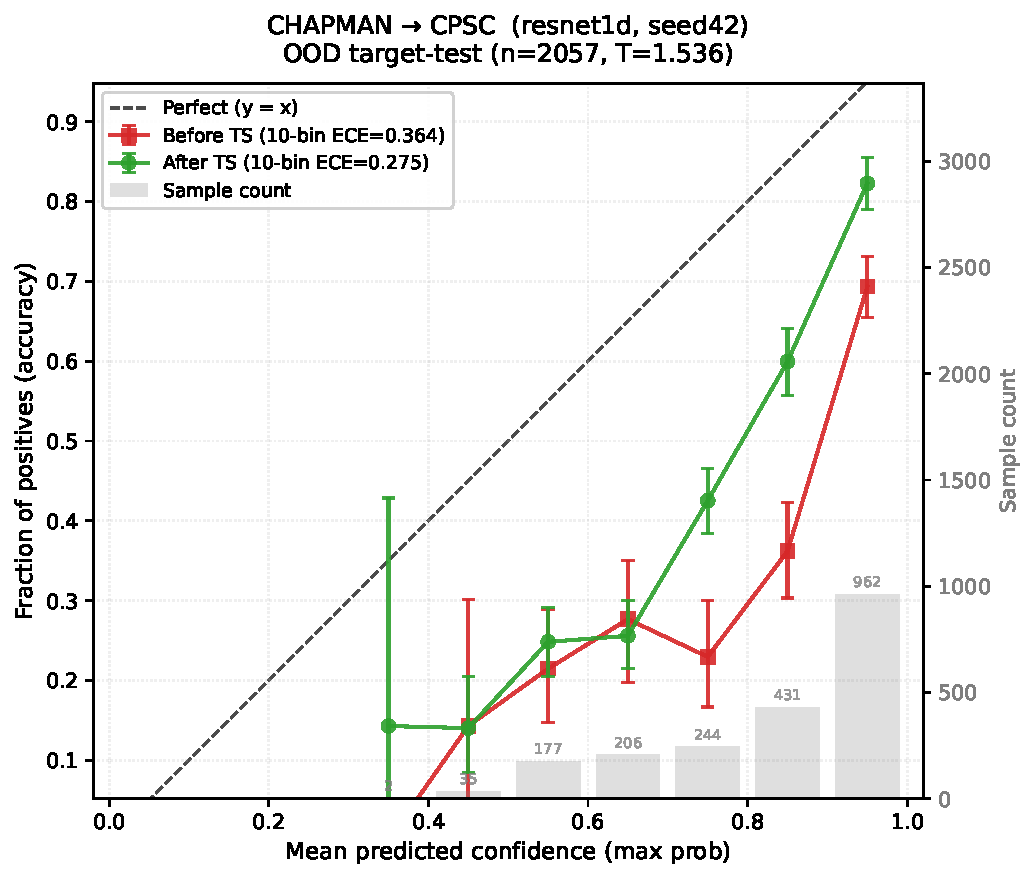
\includegraphics[width=0.32\textwidth]{figures/fig_reliability_supp_chapman_cpsc_resnet1d_seed42.pdf}
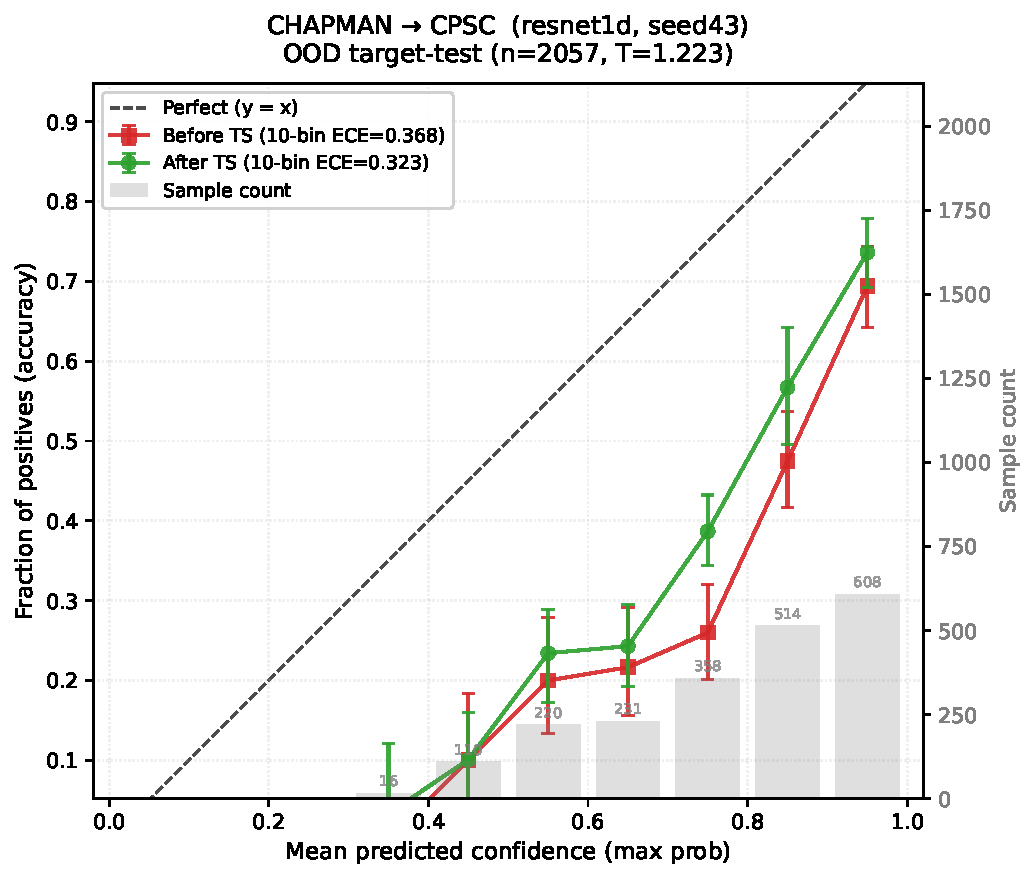
\includegraphics[width=0.32\textwidth]{figures/fig_reliability_supp_chapman_cpsc_resnet1d_seed43.pdf}
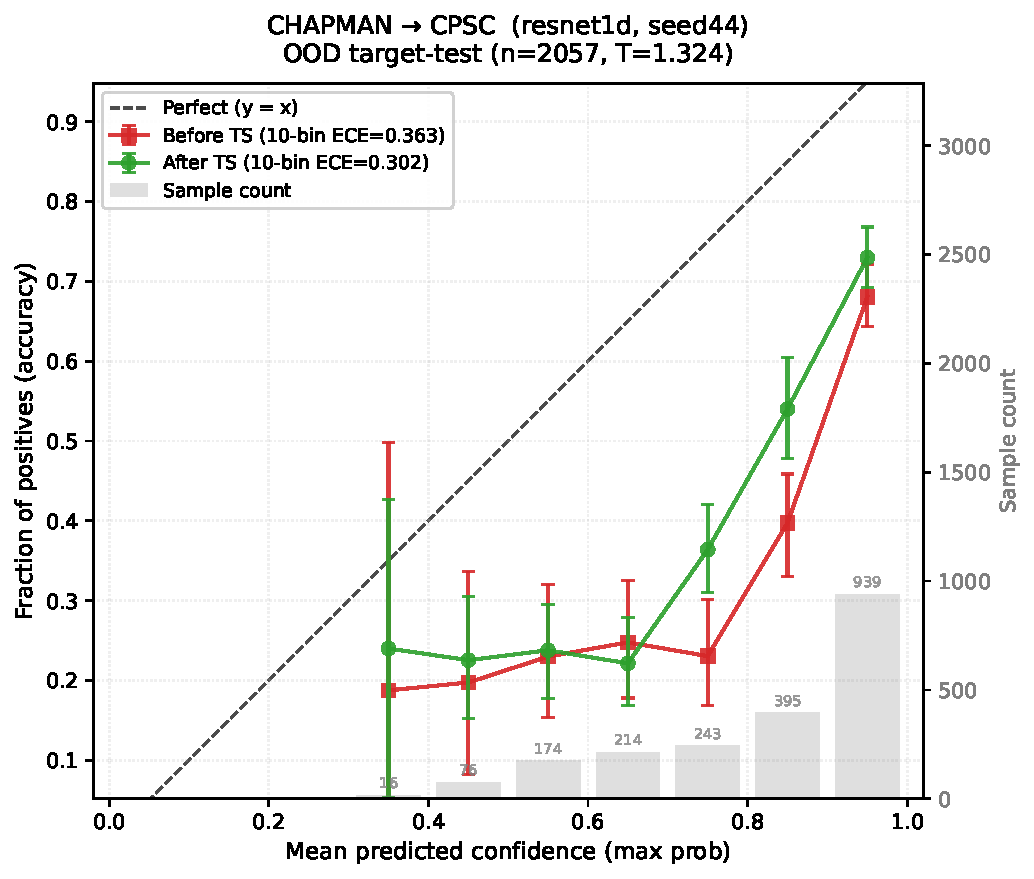
\includegraphics[width=0.32\textwidth]{figures/fig_reliability_supp_chapman_cpsc_resnet1d_seed44.pdf}
\caption{Chapman$\to$CPSC 可靠性图：ResNet1D 种子 42--44。}
\end{figure}

\begin{figure}[h]
\centering
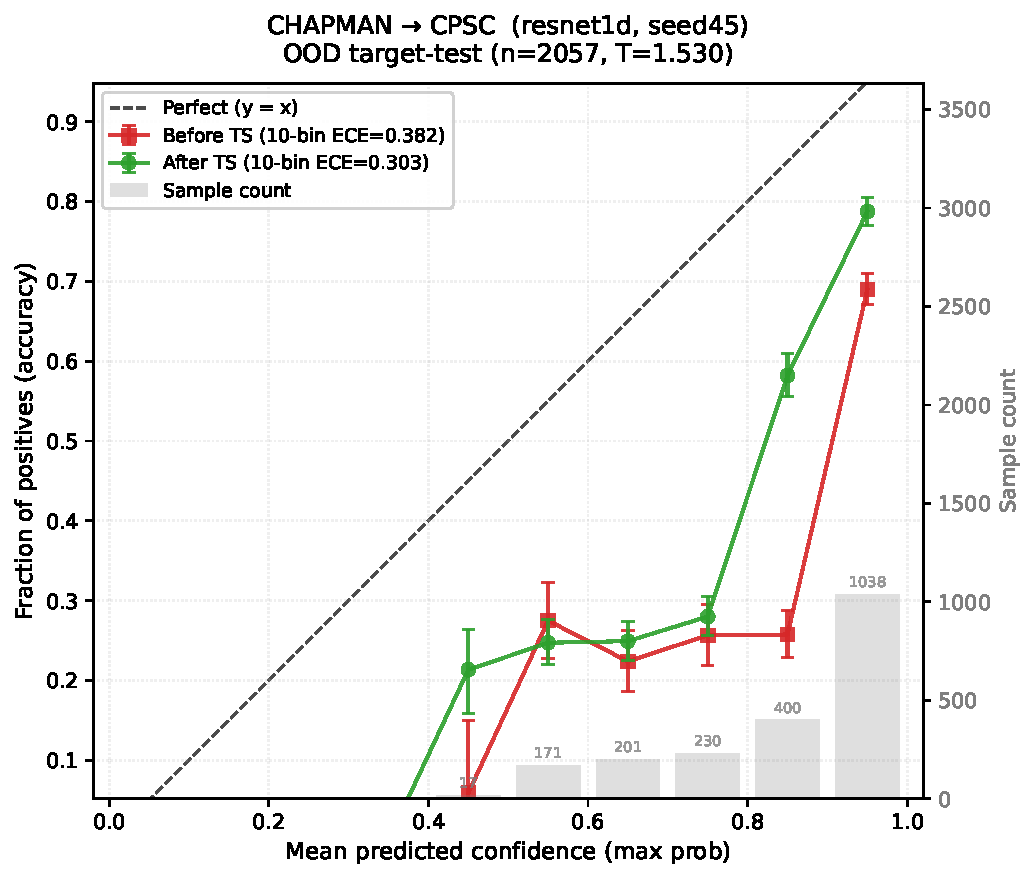
\includegraphics[width=0.45\textwidth]{figures/fig_reliability_supp_chapman_cpsc_resnet1d_seed45.pdf}
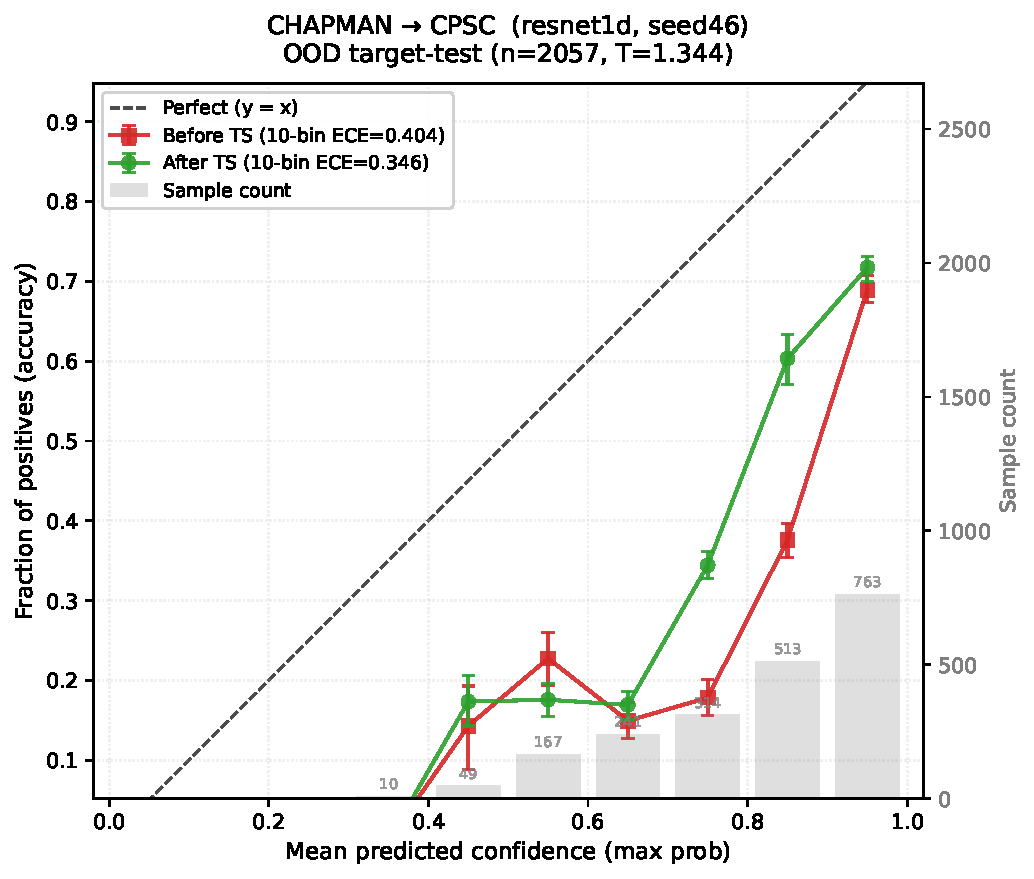
\includegraphics[width=0.45\textwidth]{figures/fig_reliability_supp_chapman_cpsc_resnet1d_seed46.pdf}
\caption{Chapman$\to$CPSC 可靠性图：ResNet1D 种子 45--46。}
\end{figure}

\begin{figure}[h]
\centering
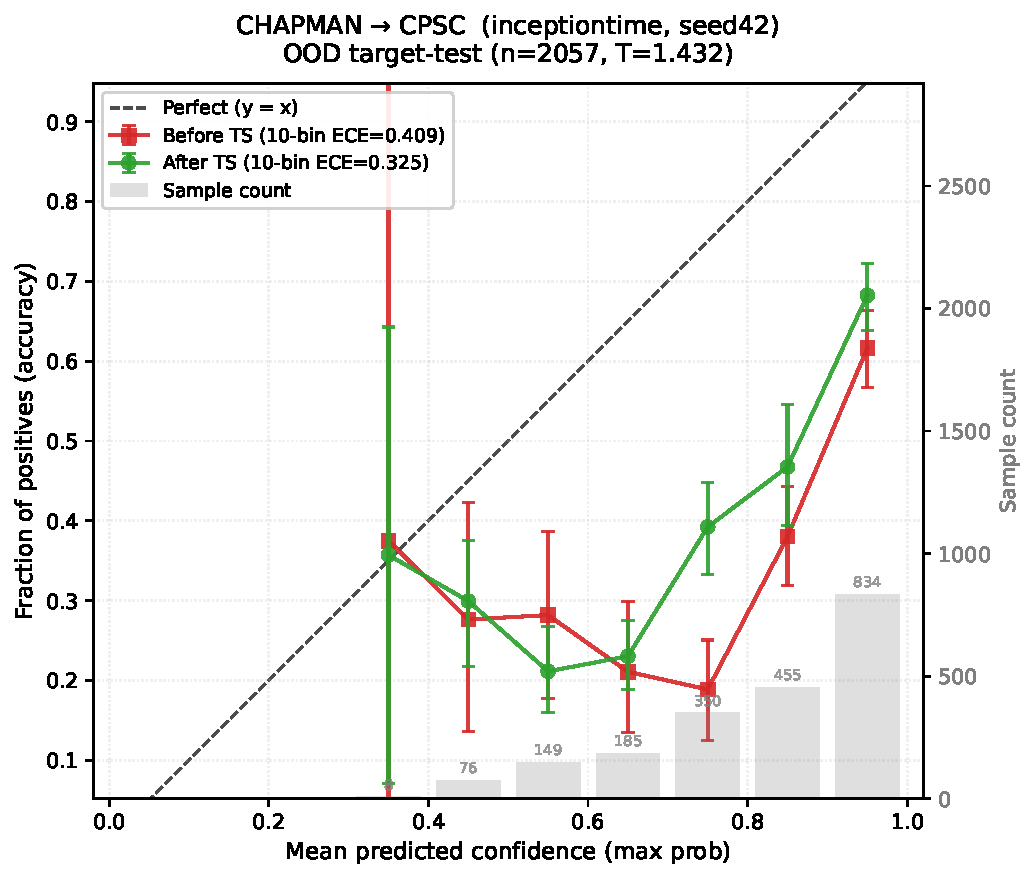
\includegraphics[width=0.32\textwidth]{figures/fig_reliability_supp_chapman_cpsc_inceptiontime_seed42.pdf}
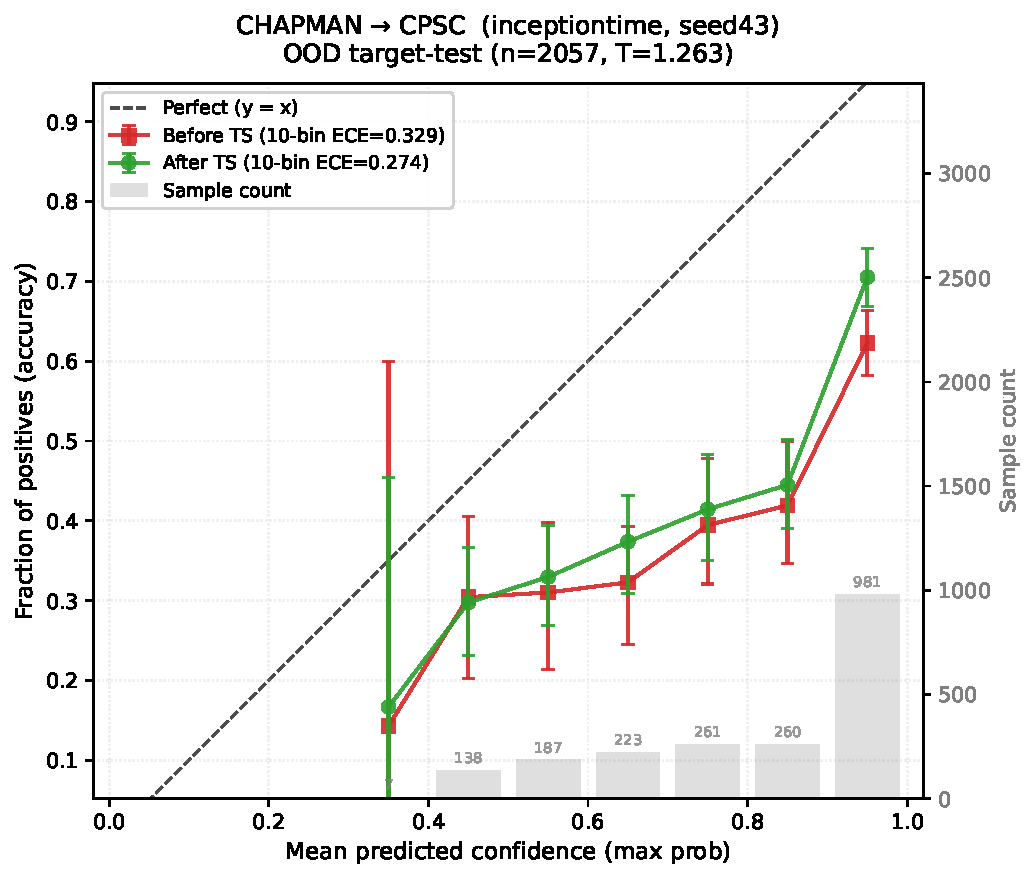
\includegraphics[width=0.32\textwidth]{figures/fig_reliability_supp_chapman_cpsc_inceptiontime_seed43.pdf}
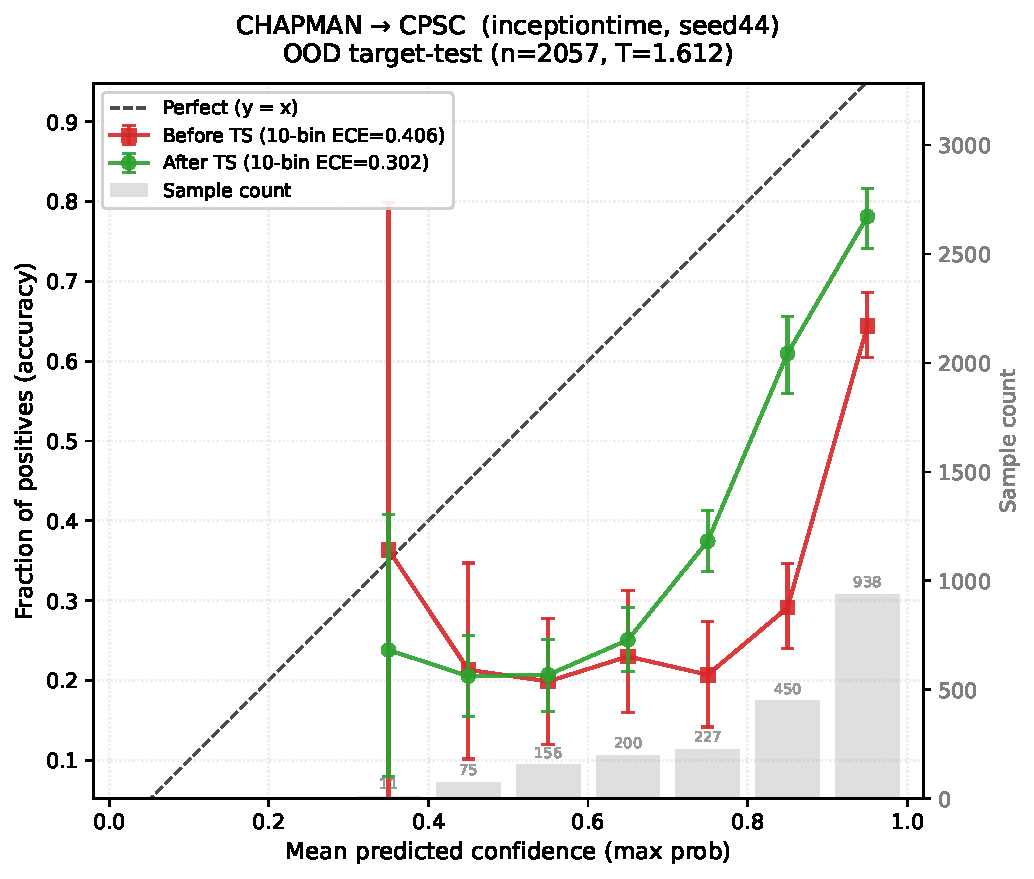
\includegraphics[width=0.32\textwidth]{figures/fig_reliability_supp_chapman_cpsc_inceptiontime_seed44.pdf}
\caption{Chapman$\to$CPSC 可靠性图：InceptionTime 种子 42--44。}
\end{figure}

\begin{figure}[h]
\centering
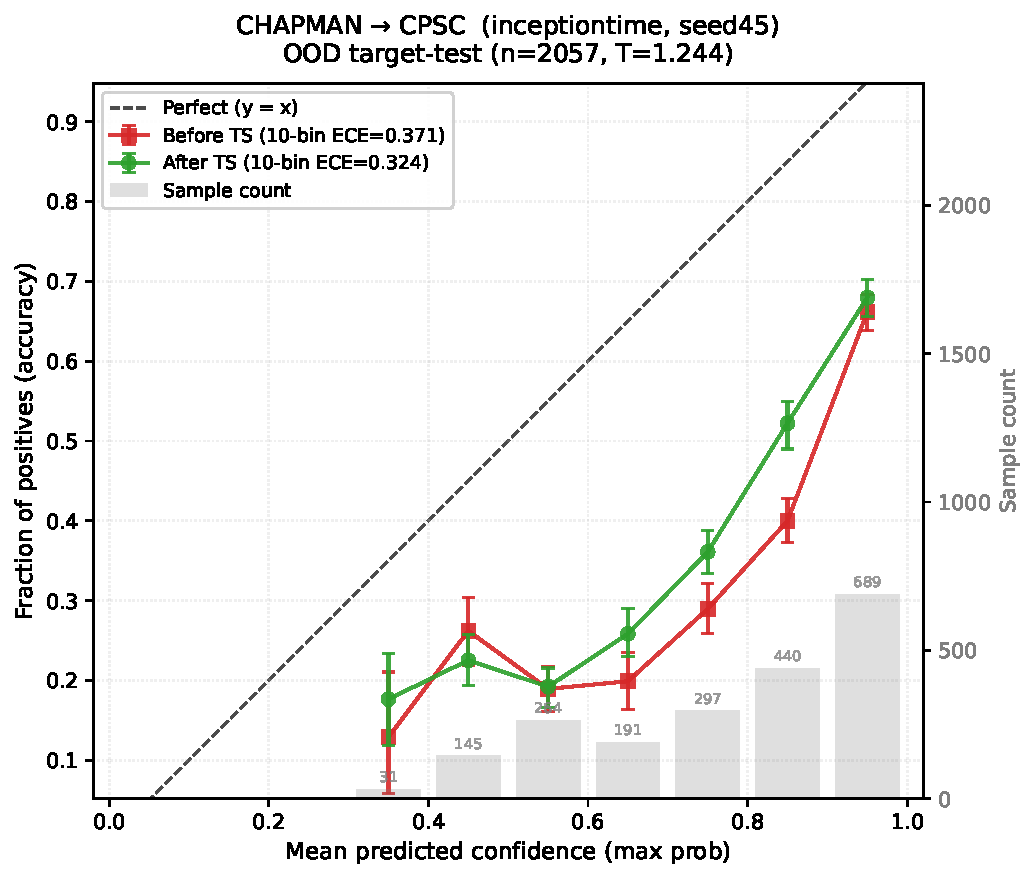
\includegraphics[width=0.45\textwidth]{figures/fig_reliability_supp_chapman_cpsc_inceptiontime_seed45.pdf}
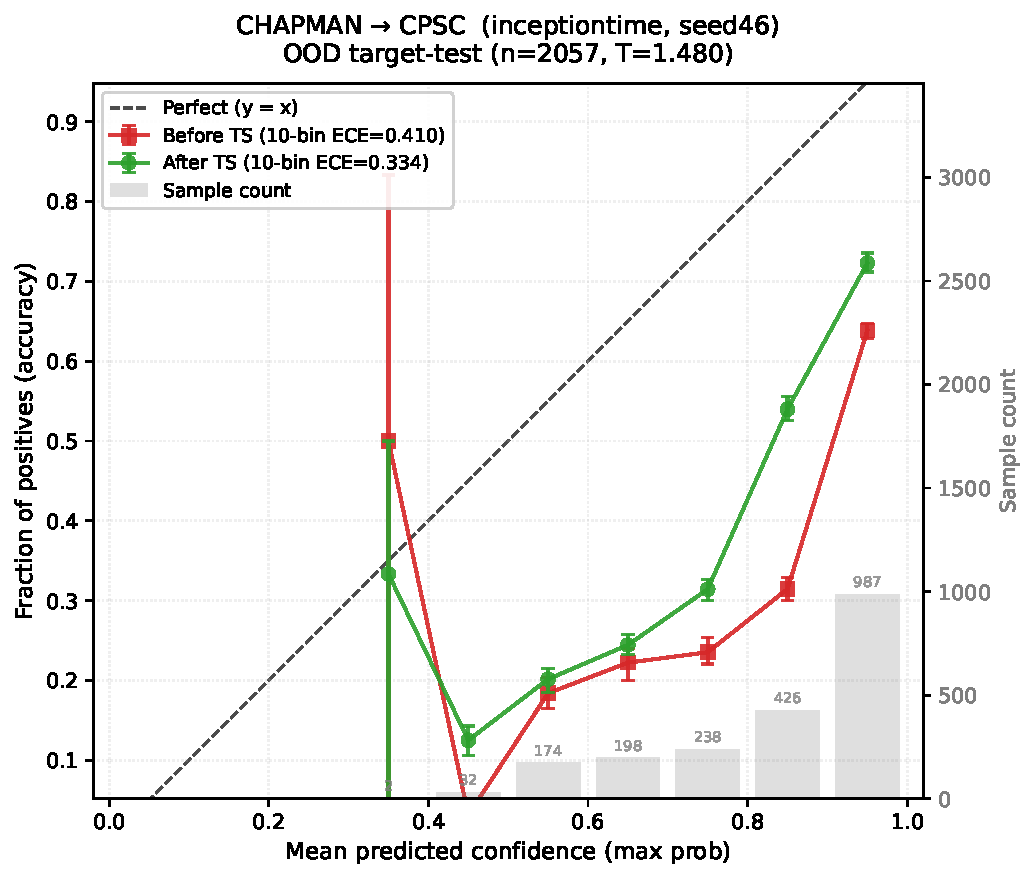
\includegraphics[width=0.45\textwidth]{figures/fig_reliability_supp_chapman_cpsc_inceptiontime_seed46.pdf}
\caption{Chapman$\to$CPSC 可靠性图：InceptionTime 种子 45--46。}
\end{figure}

\subsubsection*{S1.2.\ Chapman$\rightarrow$PTB-XL}

\begin{figure}[h]
\centering
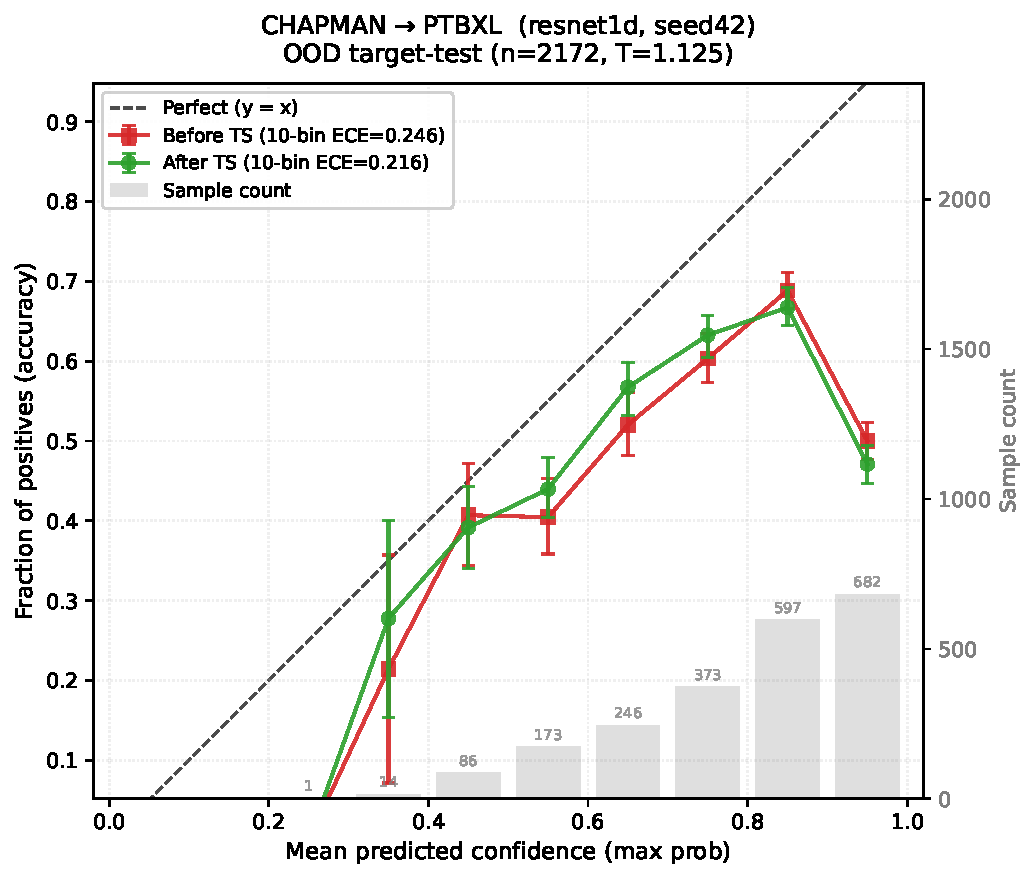
\includegraphics[width=0.32\textwidth]{figures/fig_reliability_supp_chapman_ptbxl_resnet1d_seed42.pdf}
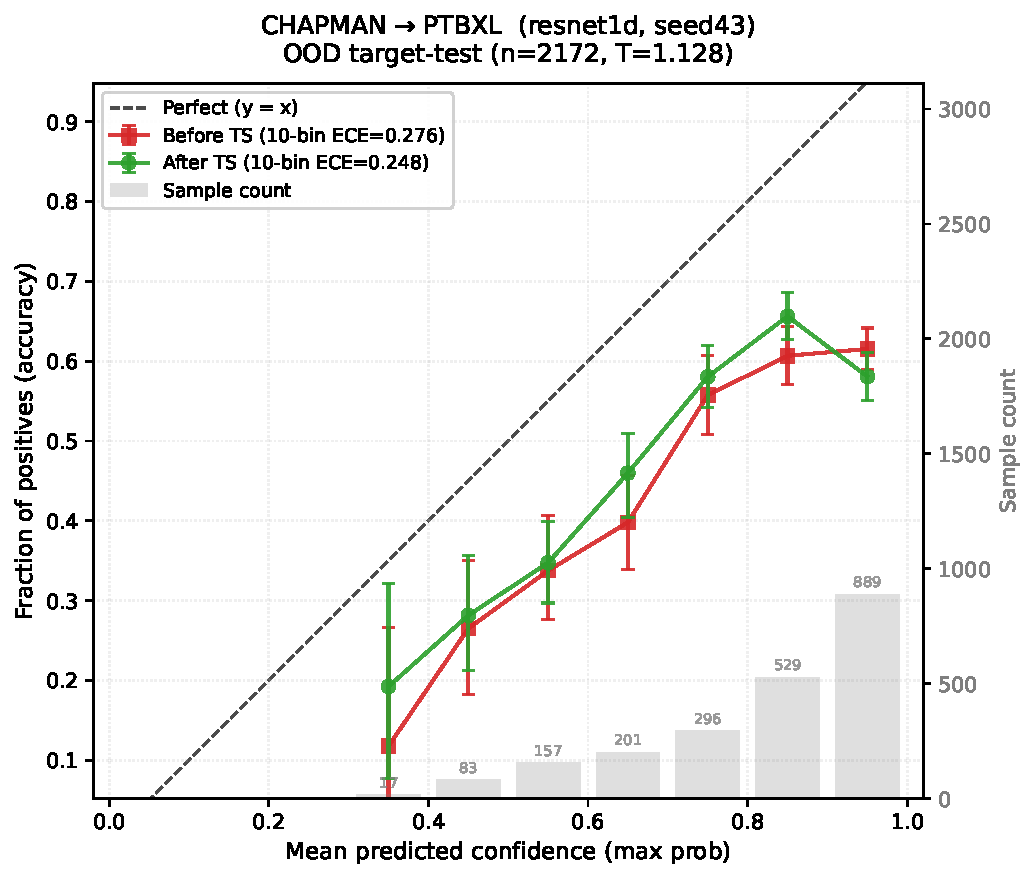
\includegraphics[width=0.32\textwidth]{figures/fig_reliability_supp_chapman_ptbxl_resnet1d_seed43.pdf}
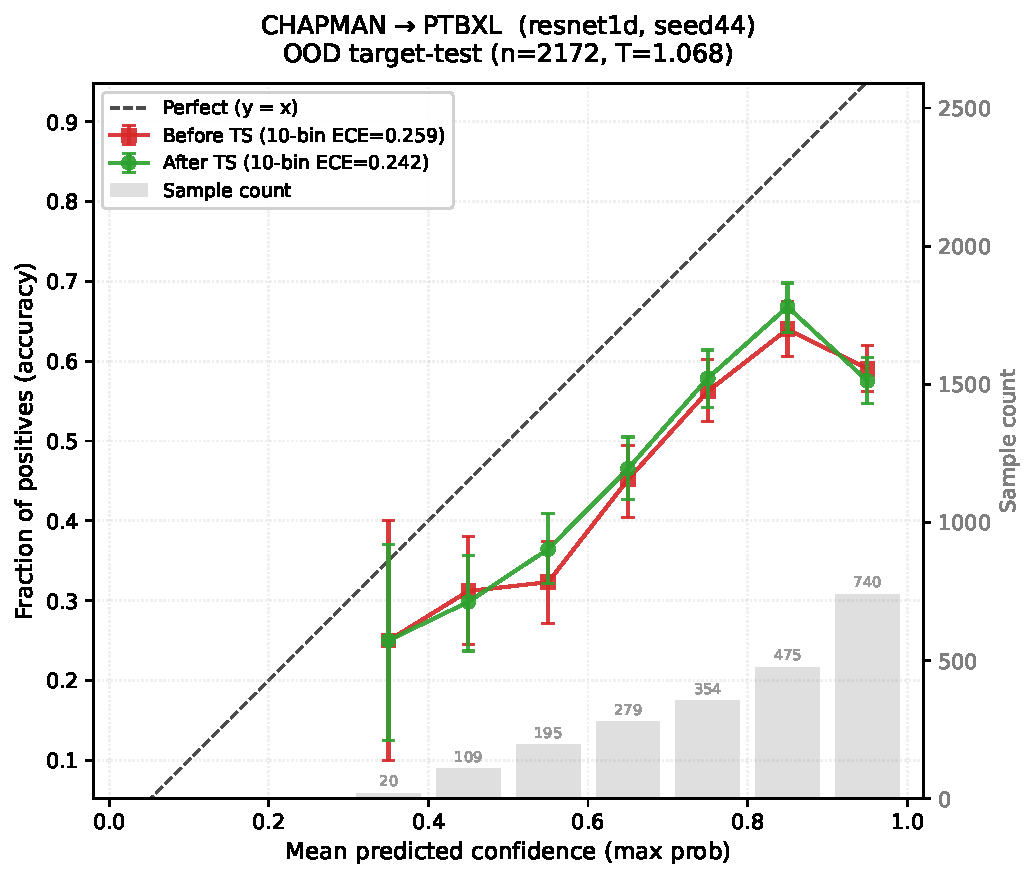
\includegraphics[width=0.32\textwidth]{figures/fig_reliability_supp_chapman_ptbxl_resnet1d_seed44.pdf}
\caption{Chapman$\to$PTB-XL 可靠性图：ResNet1D 种子 42--44。}
\end{figure}

\begin{figure}[h]
\centering
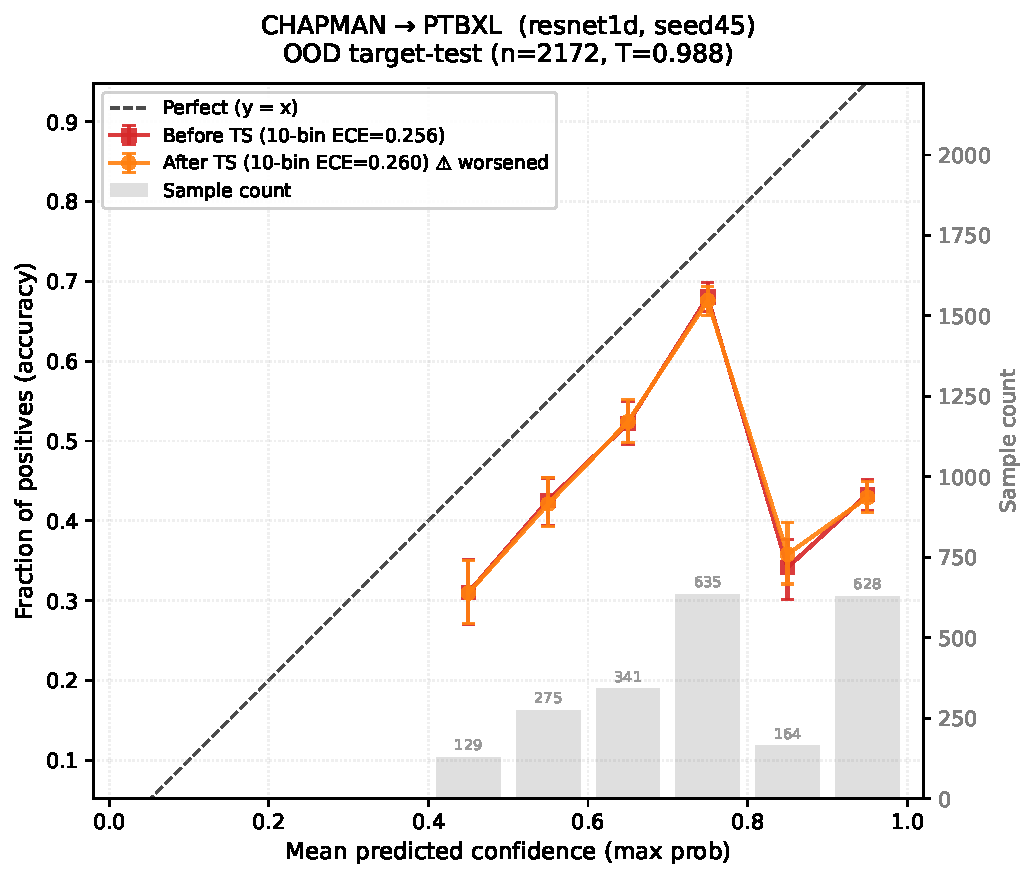
\includegraphics[width=0.45\textwidth]{figures/fig_reliability_supp_chapman_ptbxl_resnet1d_seed45.pdf}
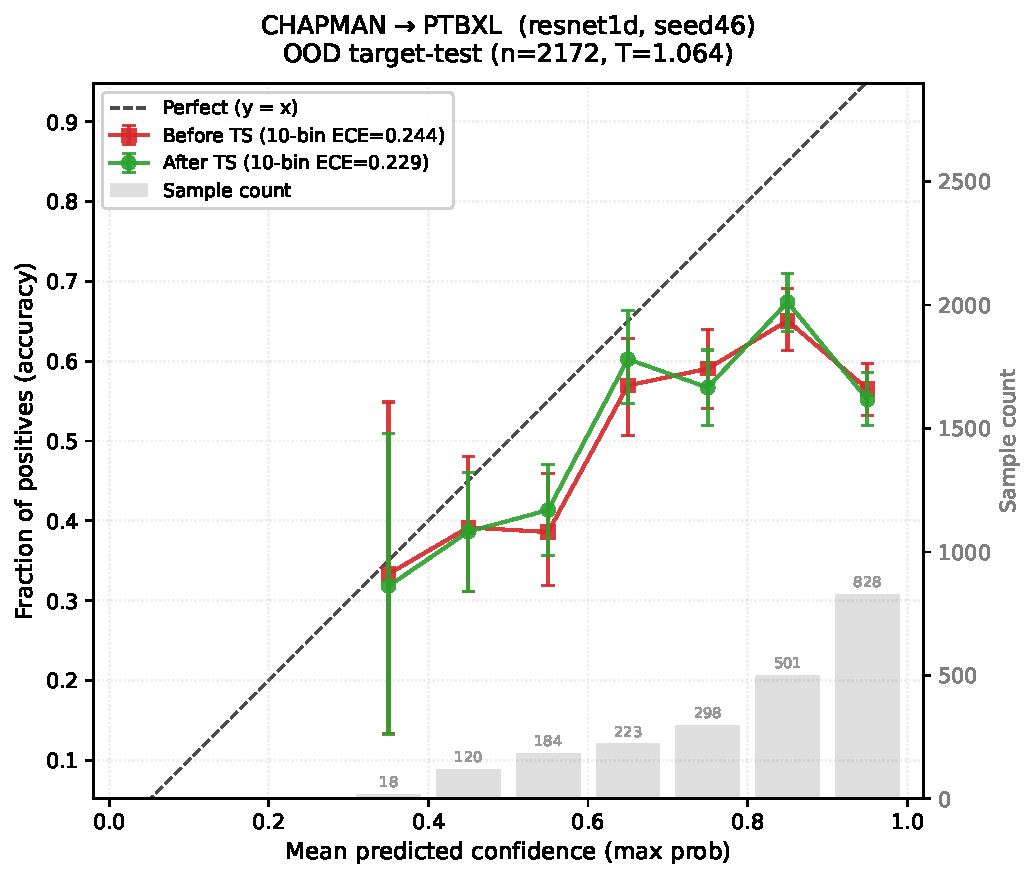
\includegraphics[width=0.45\textwidth]{figures/fig_reliability_supp_chapman_ptbxl_resnet1d_seed46.pdf}
\caption{Chapman$\to$PTB-XL 可靠性图：ResNet1D 种子 45--46。}
\end{figure}

\begin{figure}[h]
\centering
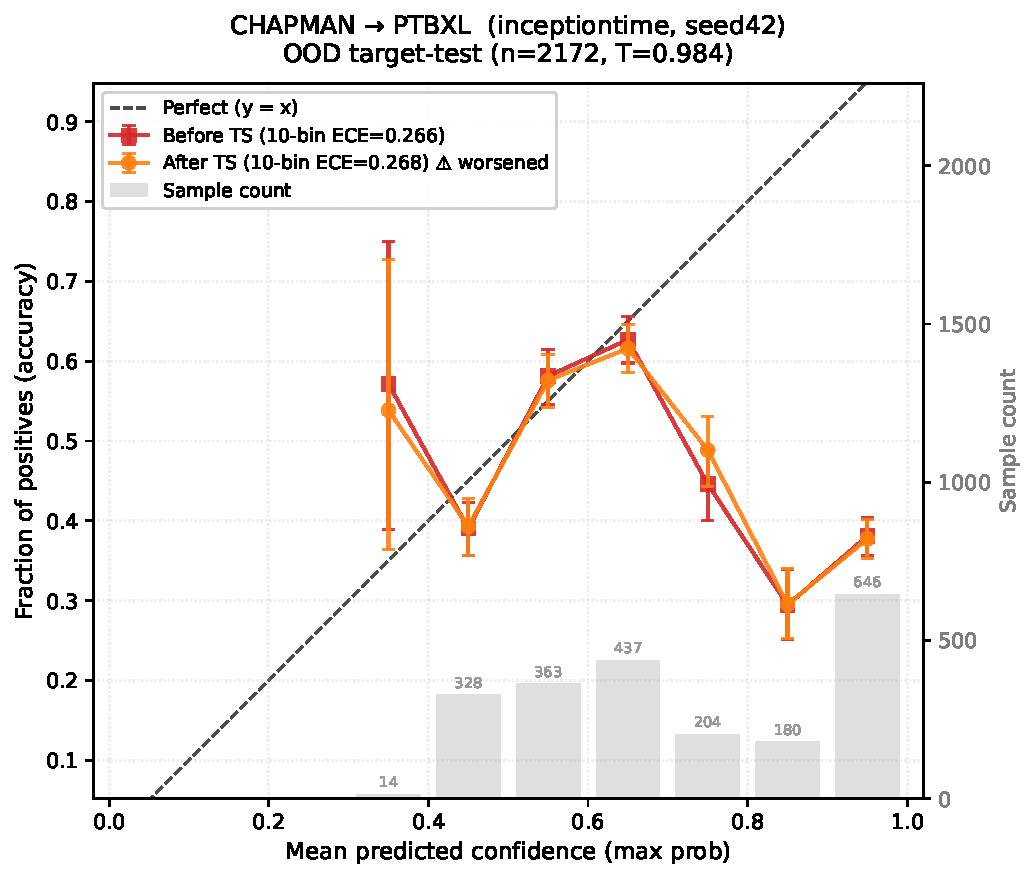
\includegraphics[width=0.32\textwidth]{figures/fig_reliability_supp_chapman_ptbxl_inceptiontime_seed42.pdf}
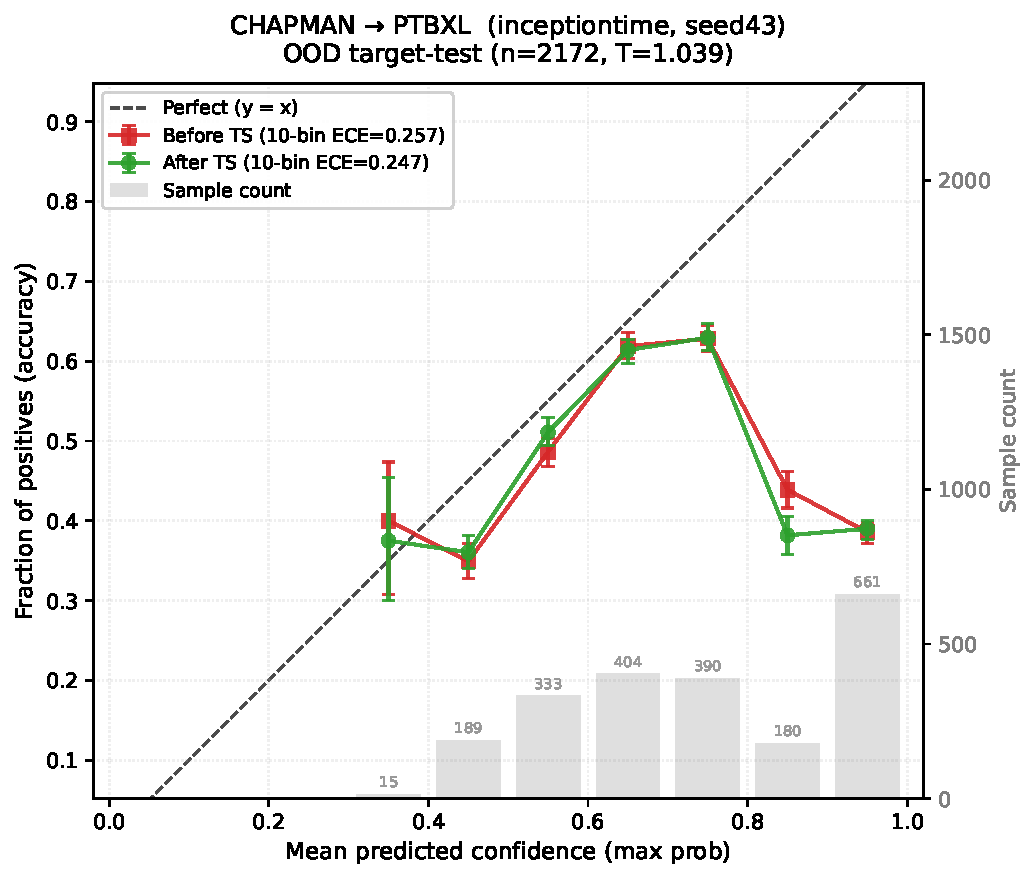
\includegraphics[width=0.32\textwidth]{figures/fig_reliability_supp_chapman_ptbxl_inceptiontime_seed43.pdf}
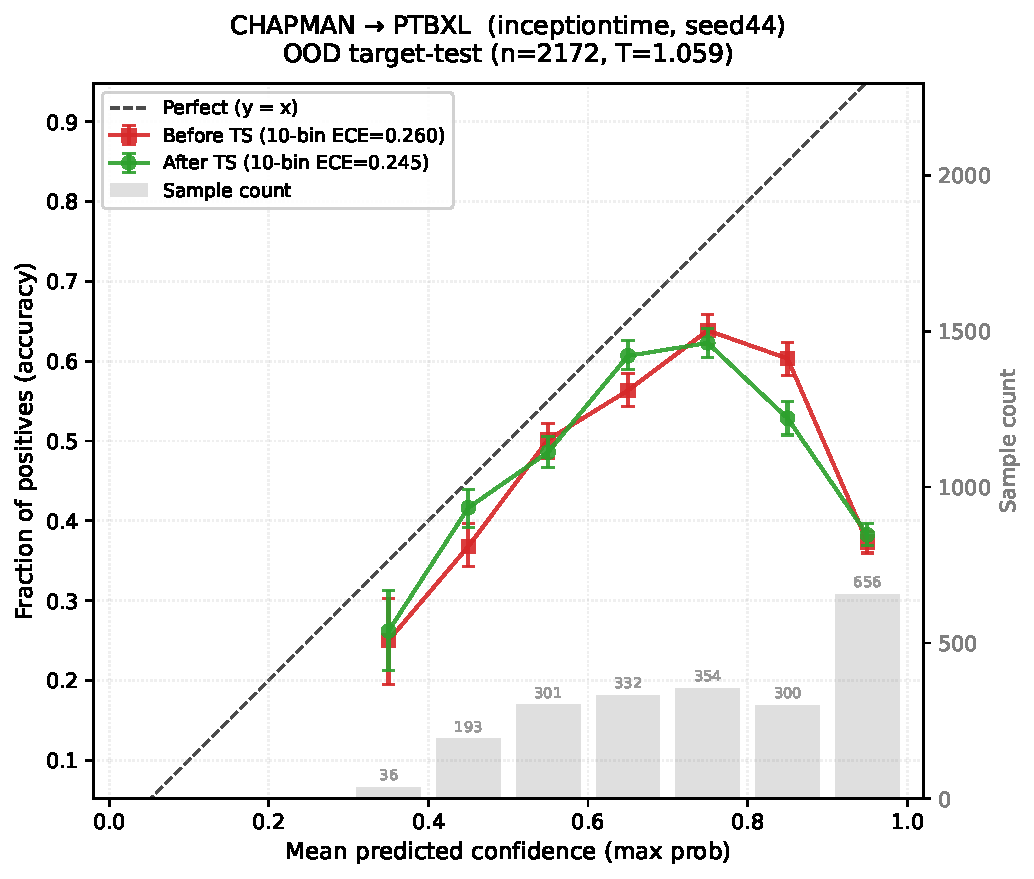
\includegraphics[width=0.32\textwidth]{figures/fig_reliability_supp_chapman_ptbxl_inceptiontime_seed44.pdf}
\caption{Chapman$\to$PTB-XL 可靠性图：InceptionTime 种子 42--44。}
\end{figure}

\begin{figure}[h]
\centering
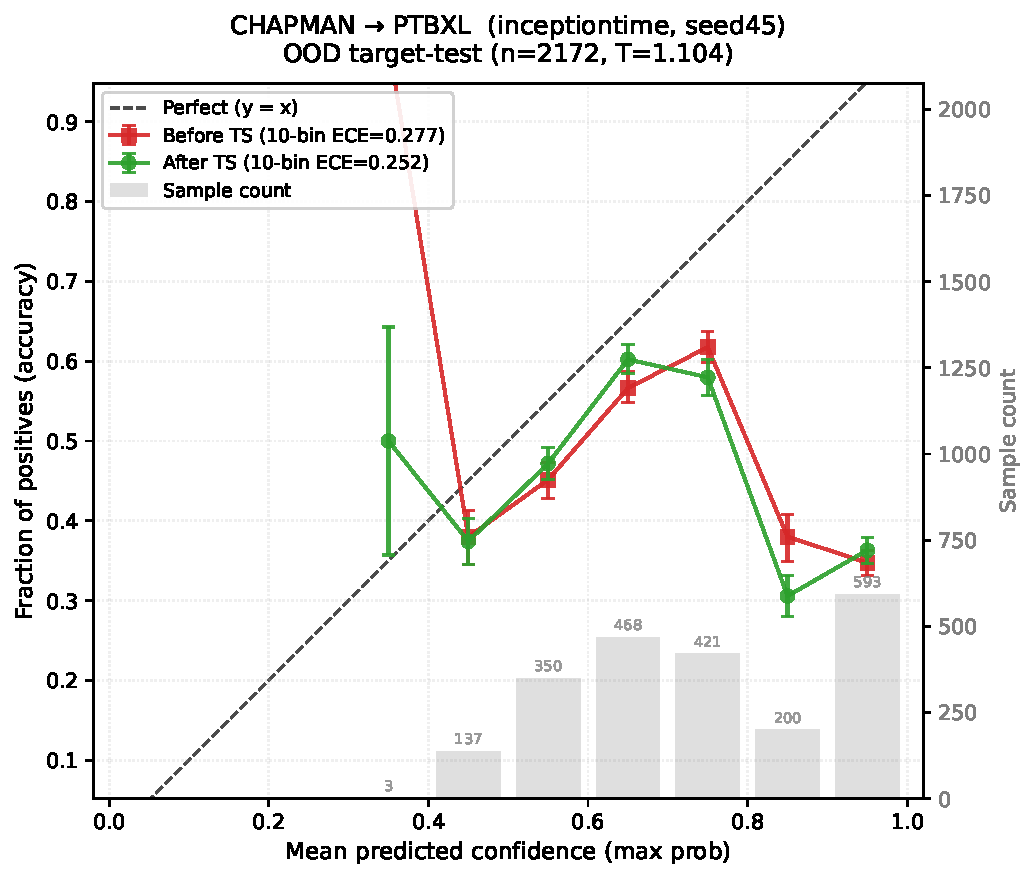
\includegraphics[width=0.45\textwidth]{figures/fig_reliability_supp_chapman_ptbxl_inceptiontime_seed45.pdf}
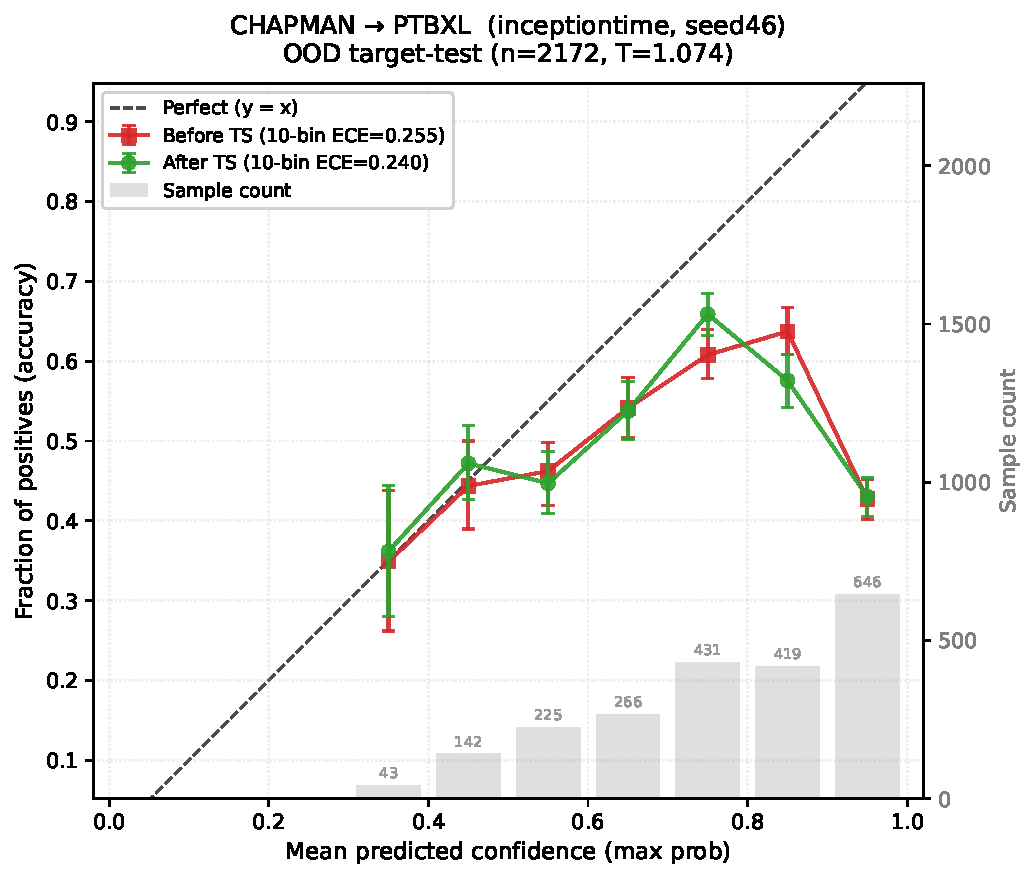
\includegraphics[width=0.45\textwidth]{figures/fig_reliability_supp_chapman_ptbxl_inceptiontime_seed46.pdf}
\caption{Chapman$\to$PTB-XL 可靠性图：InceptionTime 种子 45--46。}
\end{figure}

\subsubsection*{S1.3.\ CPSC$\rightarrow$Chapman}

\begin{figure}[h]
\centering
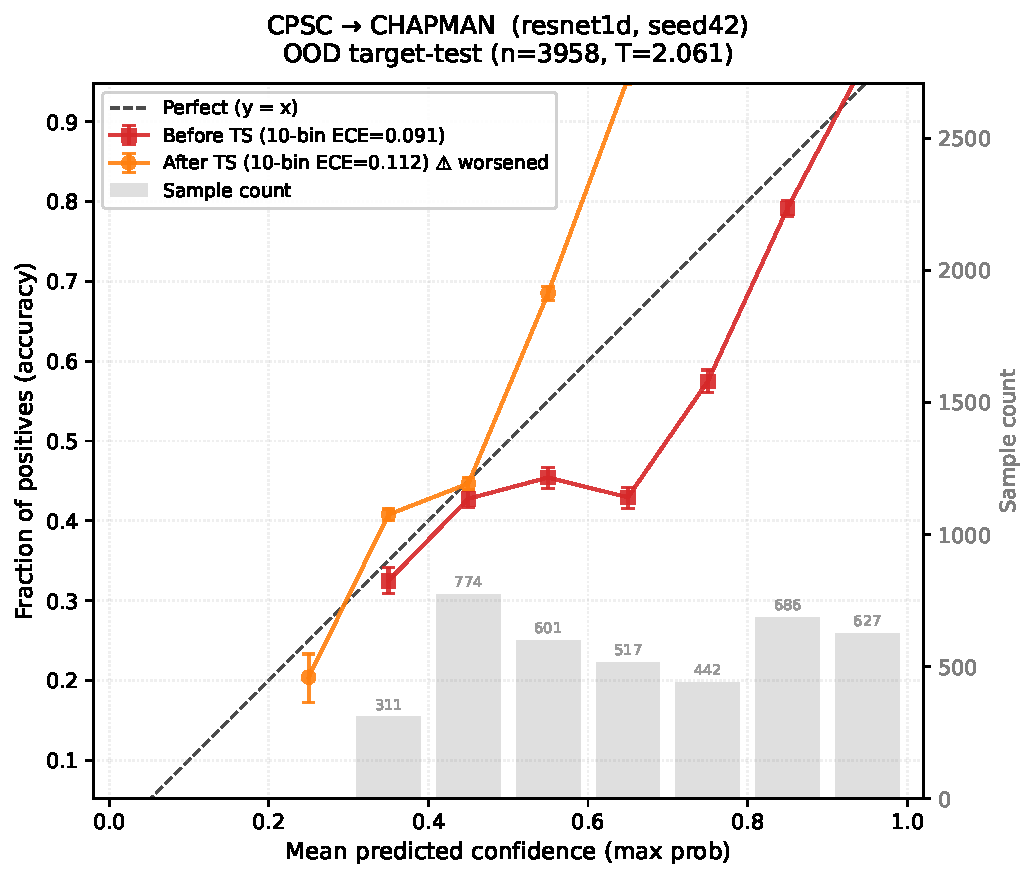
\includegraphics[width=0.32\textwidth]{figures/fig_reliability_supp_cpsc_chapman_resnet1d_seed42.pdf}
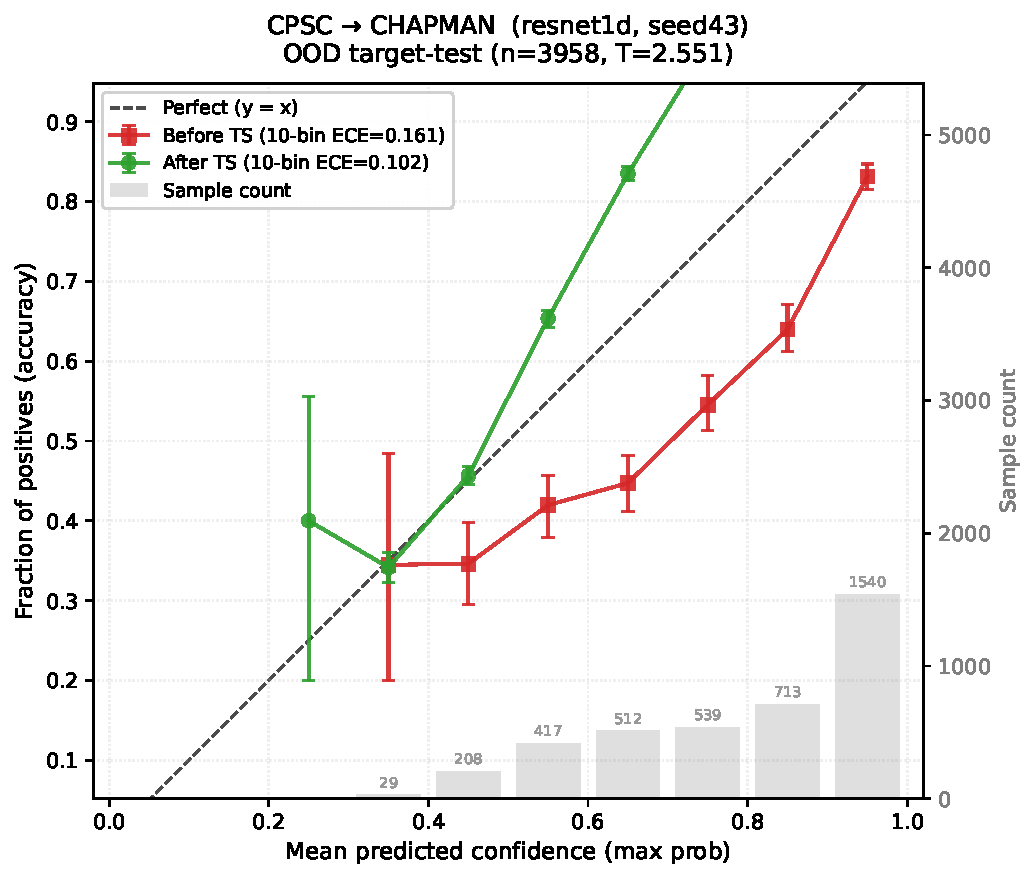
\includegraphics[width=0.32\textwidth]{figures/fig_reliability_supp_cpsc_chapman_resnet1d_seed43.pdf}
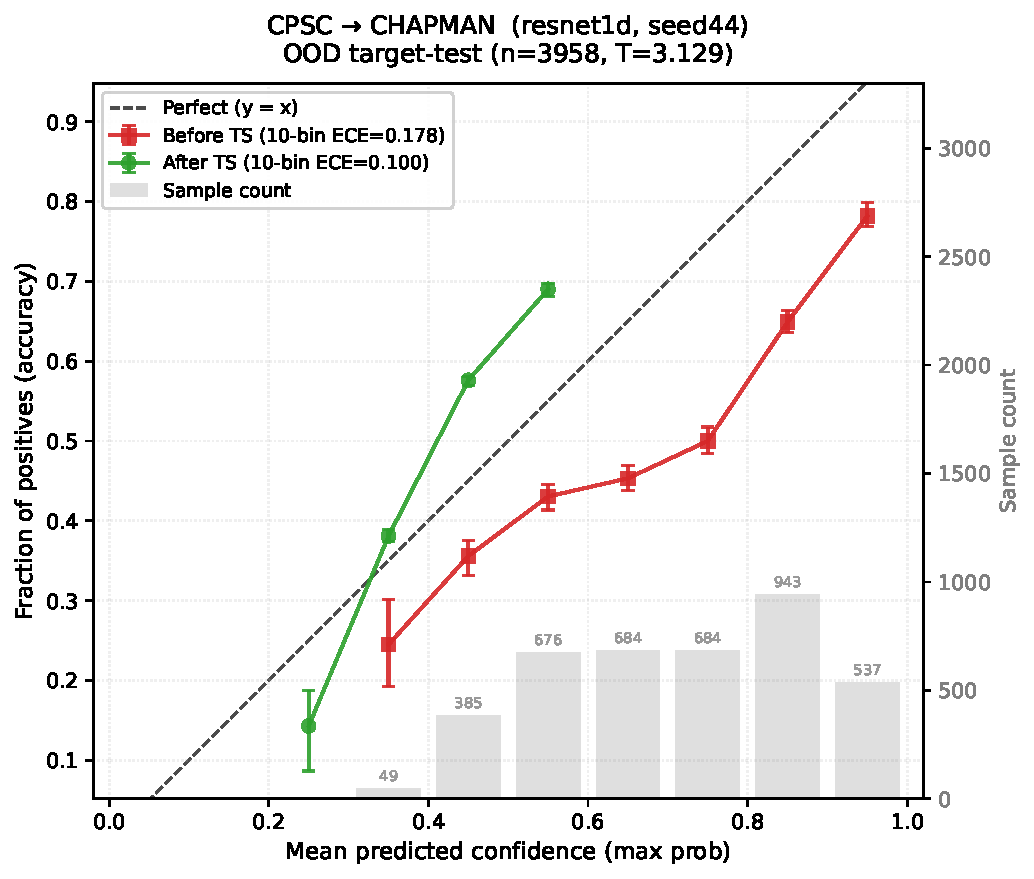
\includegraphics[width=0.32\textwidth]{figures/fig_reliability_supp_cpsc_chapman_resnet1d_seed44.pdf}
\caption{CPSC$\to$Chapman 可靠性图：ResNet1D 种子 42--44。}
\end{figure}

\begin{figure}[h]
\centering
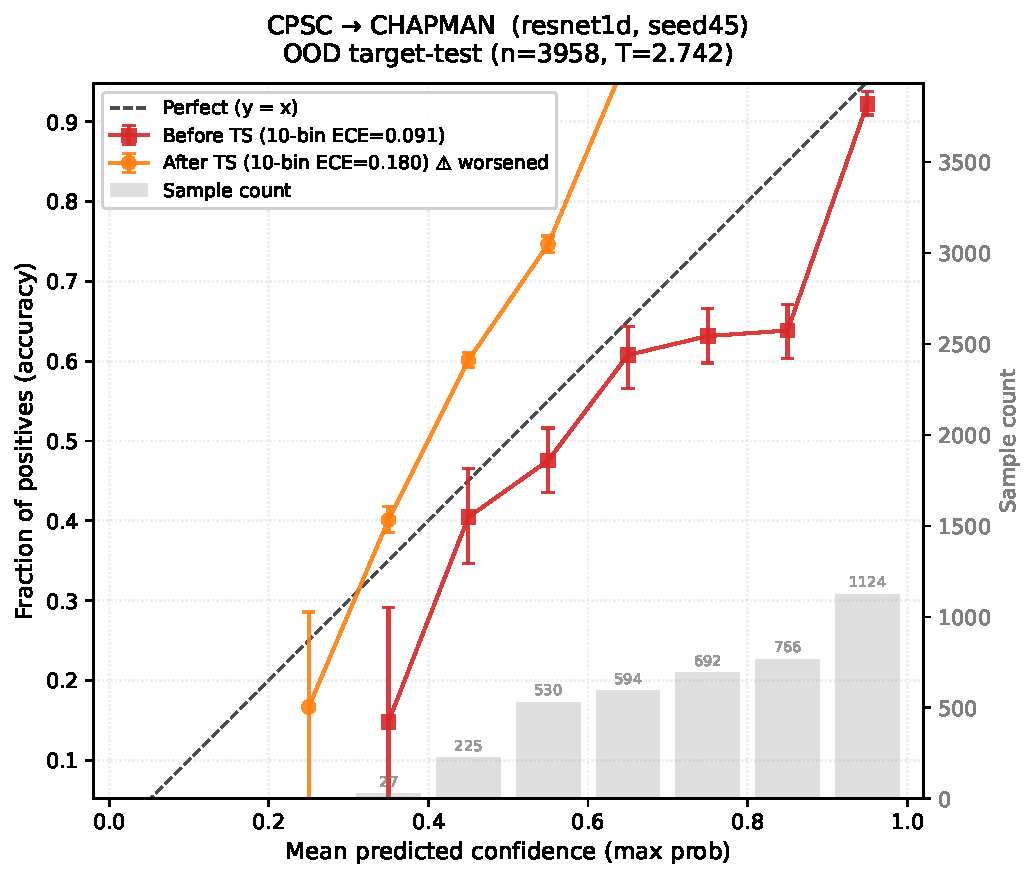
\includegraphics[width=0.45\textwidth]{figures/fig_reliability_supp_cpsc_chapman_resnet1d_seed45.pdf}
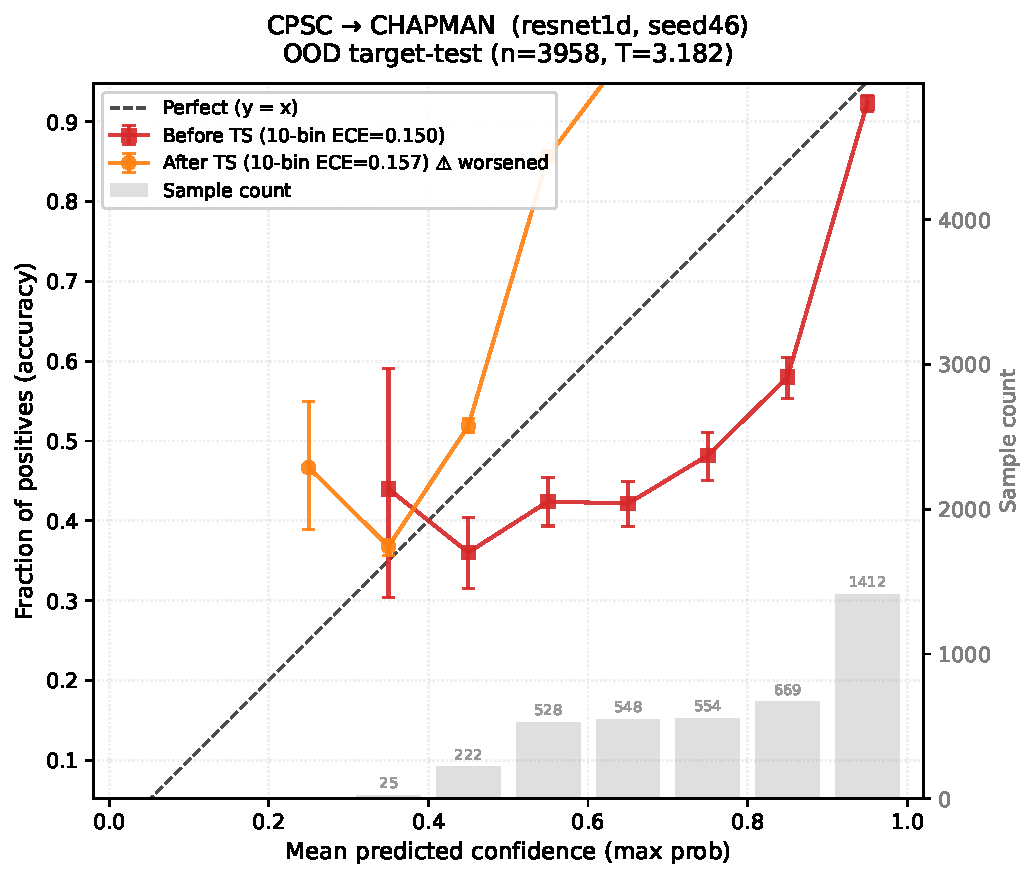
\includegraphics[width=0.45\textwidth]{figures/fig_reliability_supp_cpsc_chapman_resnet1d_seed46.pdf}
\caption{CPSC$\to$Chapman 可靠性图：ResNet1D 种子 45--46。}
\end{figure}

\begin{figure}[h]
\centering
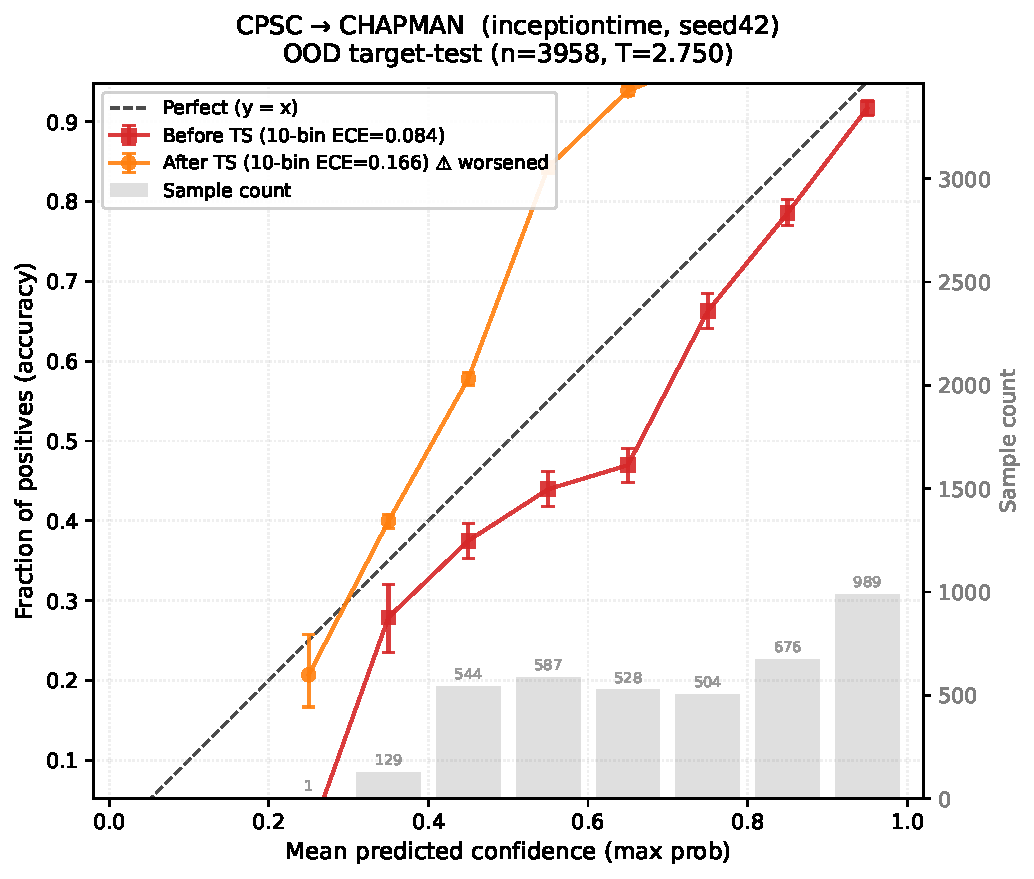
\includegraphics[width=0.32\textwidth]{figures/fig_reliability_supp_cpsc_chapman_inceptiontime_seed42.pdf}
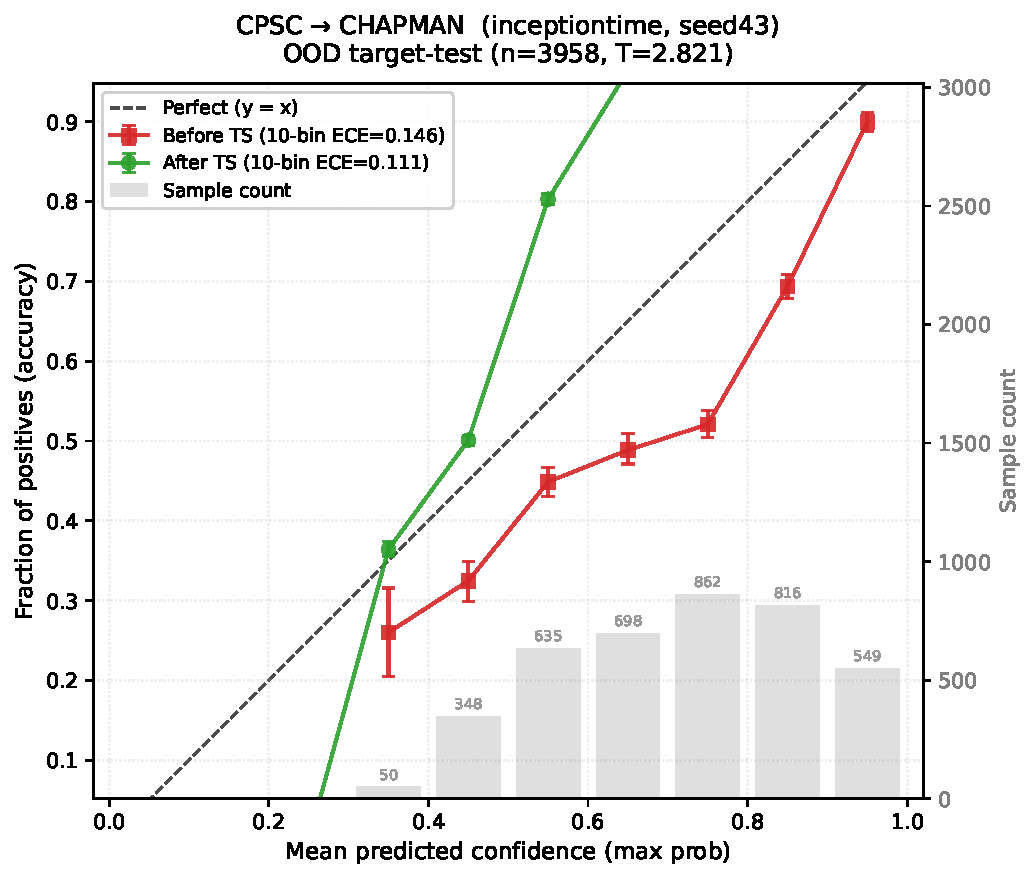
\includegraphics[width=0.32\textwidth]{figures/fig_reliability_supp_cpsc_chapman_inceptiontime_seed43.pdf}
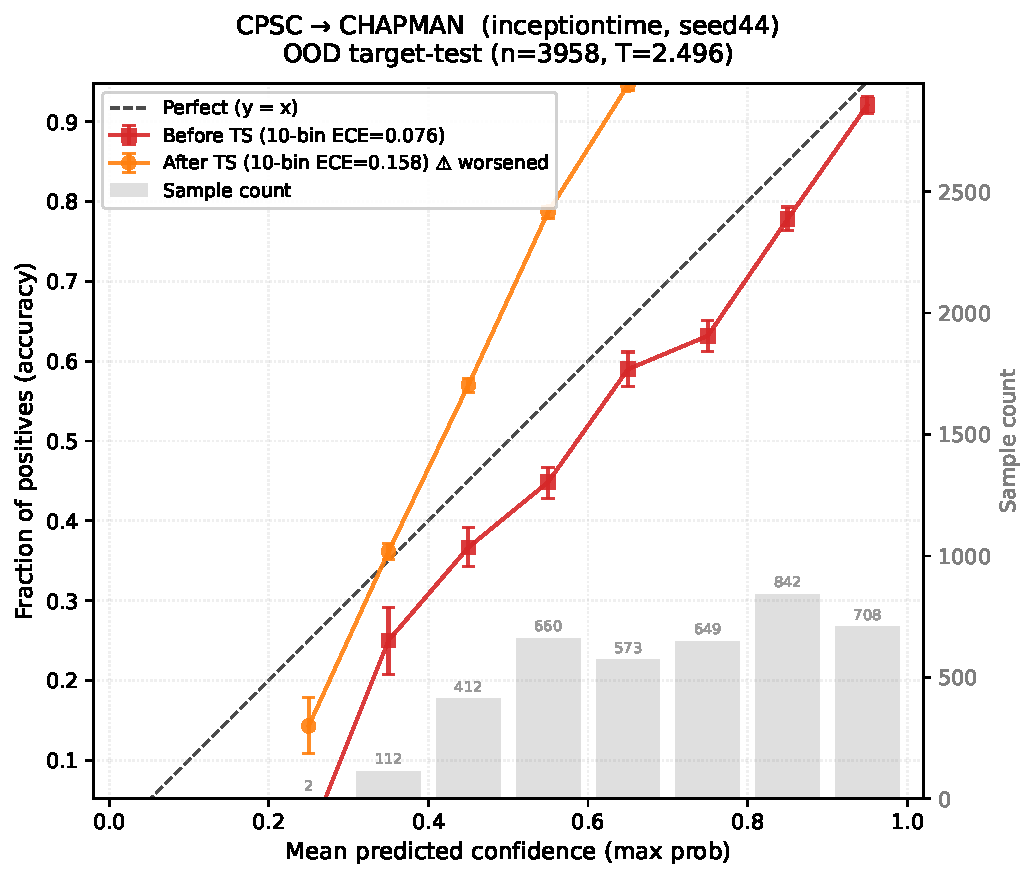
\includegraphics[width=0.32\textwidth]{figures/fig_reliability_supp_cpsc_chapman_inceptiontime_seed44.pdf}
\caption{CPSC$\to$Chapman 可靠性图：InceptionTime 种子 42--44。}
\end{figure}

\begin{figure}[h]
\centering
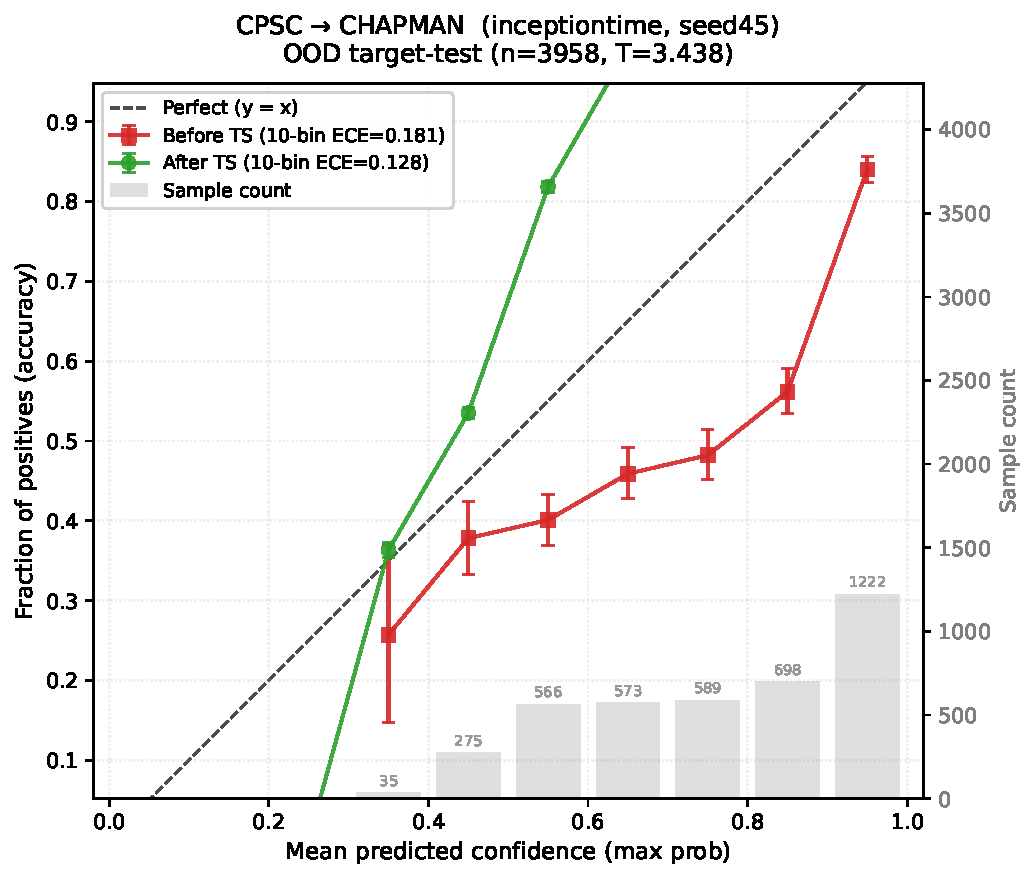
\includegraphics[width=0.45\textwidth]{figures/fig_reliability_supp_cpsc_chapman_inceptiontime_seed45.pdf}
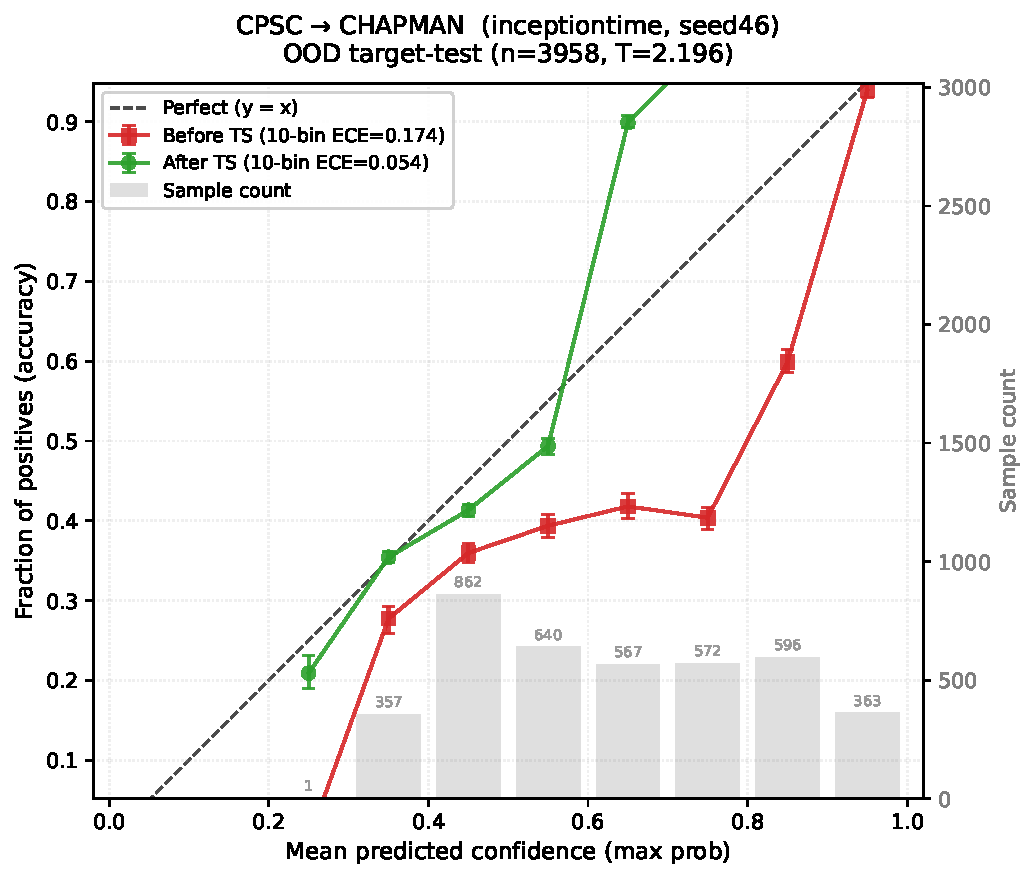
\includegraphics[width=0.45\textwidth]{figures/fig_reliability_supp_cpsc_chapman_inceptiontime_seed46.pdf}
\caption{CPSC$\to$Chapman 可靠性图：InceptionTime 种子 45--46。}
\end{figure}

\subsubsection*{S1.4.\ CPSC$\rightarrow$PTB-XL}

\begin{figure}[h]
\centering
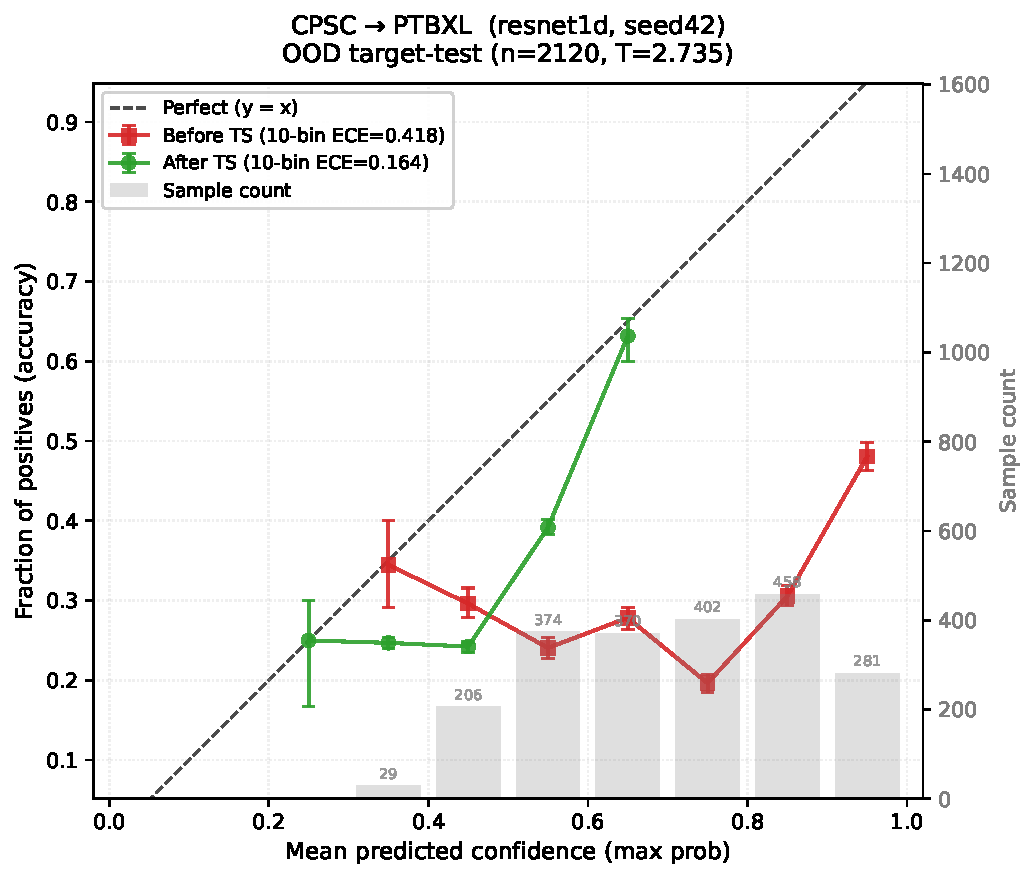
\includegraphics[width=0.32\textwidth]{figures/fig_reliability_supp_cpsc_ptbxl_resnet1d_seed42.pdf}
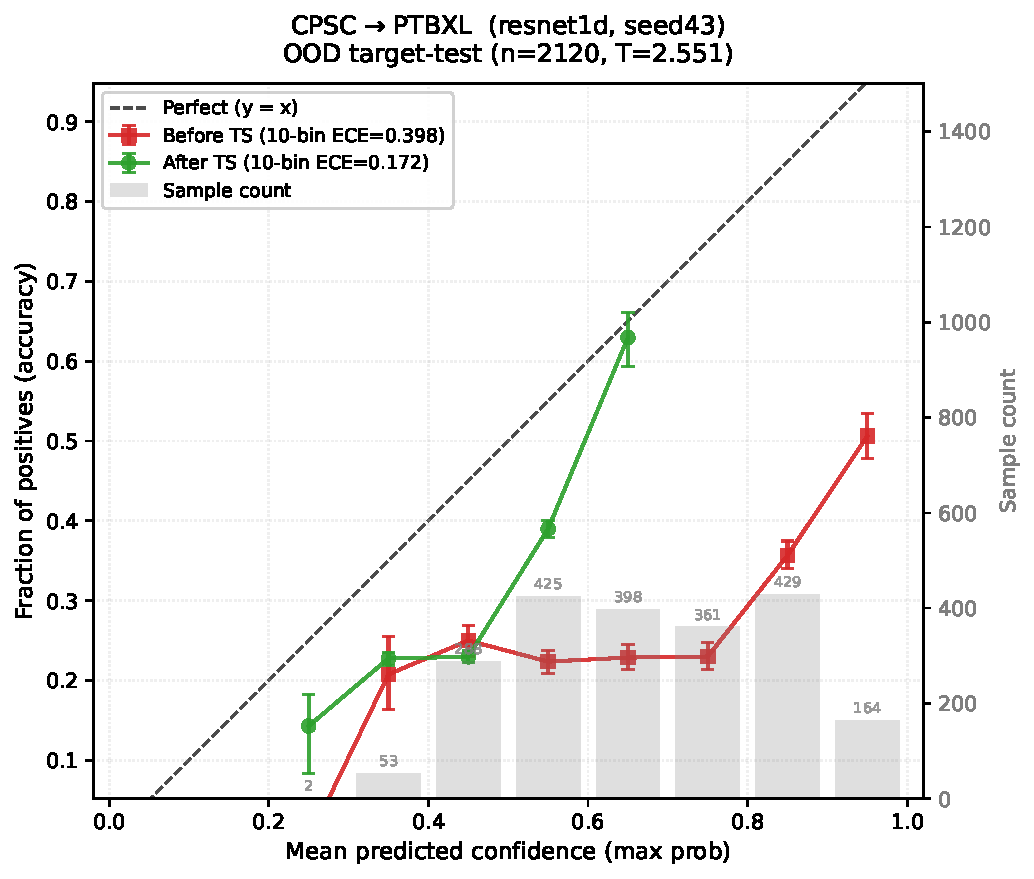
\includegraphics[width=0.32\textwidth]{figures/fig_reliability_supp_cpsc_ptbxl_resnet1d_seed43.pdf}
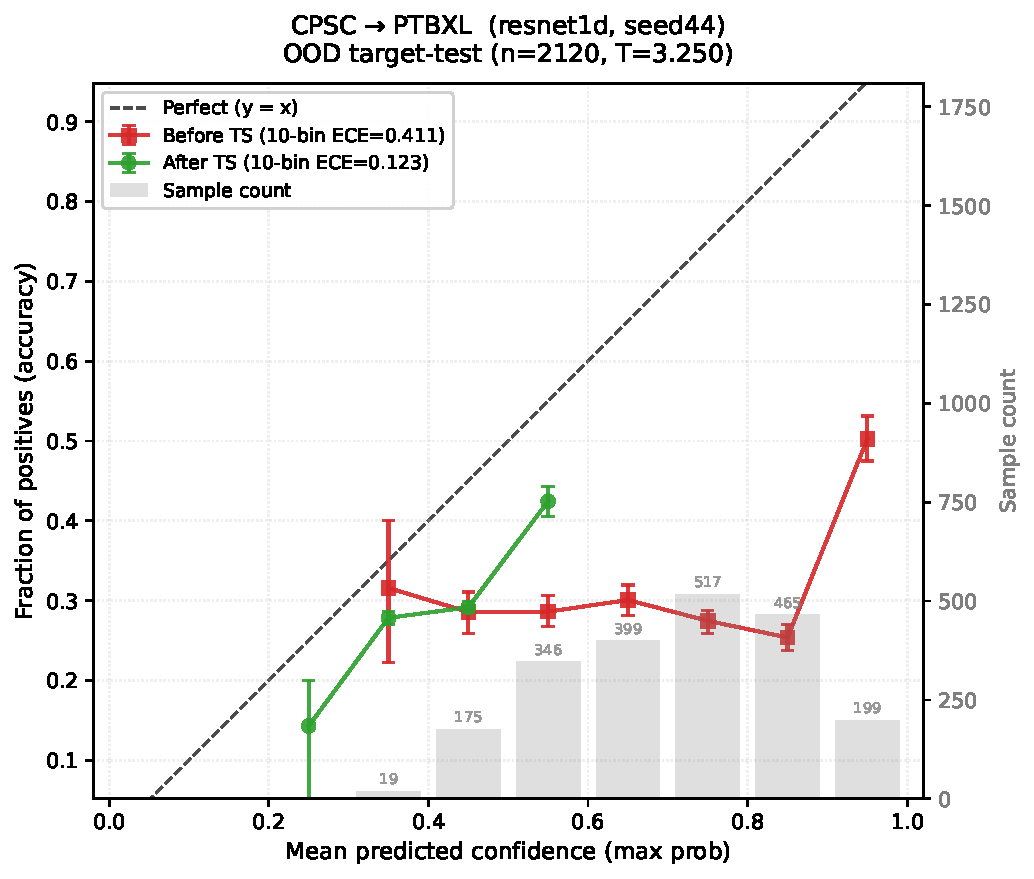
\includegraphics[width=0.32\textwidth]{figures/fig_reliability_supp_cpsc_ptbxl_resnet1d_seed44.pdf}
\caption{CPSC$\to$PTB-XL 可靠性图：ResNet1D 种子 42--44。}
\end{figure}

\begin{figure}[h]
\centering
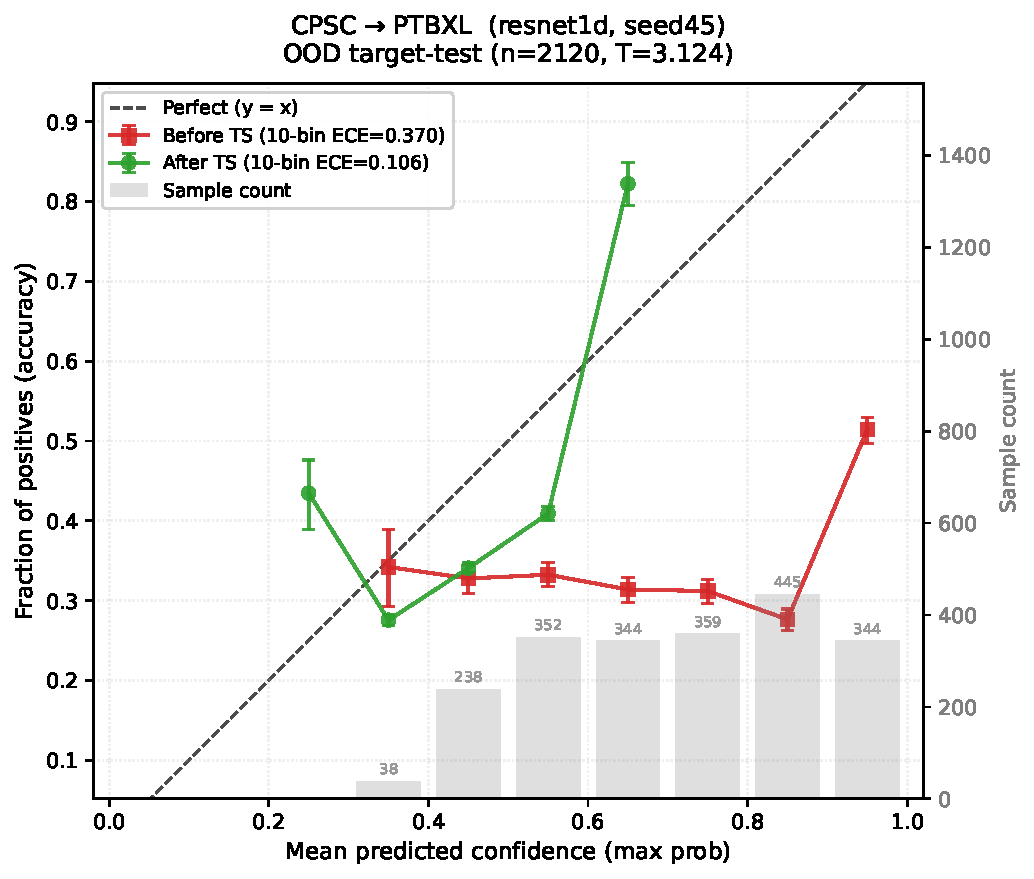
\includegraphics[width=0.45\textwidth]{figures/fig_reliability_supp_cpsc_ptbxl_resnet1d_seed45.pdf}
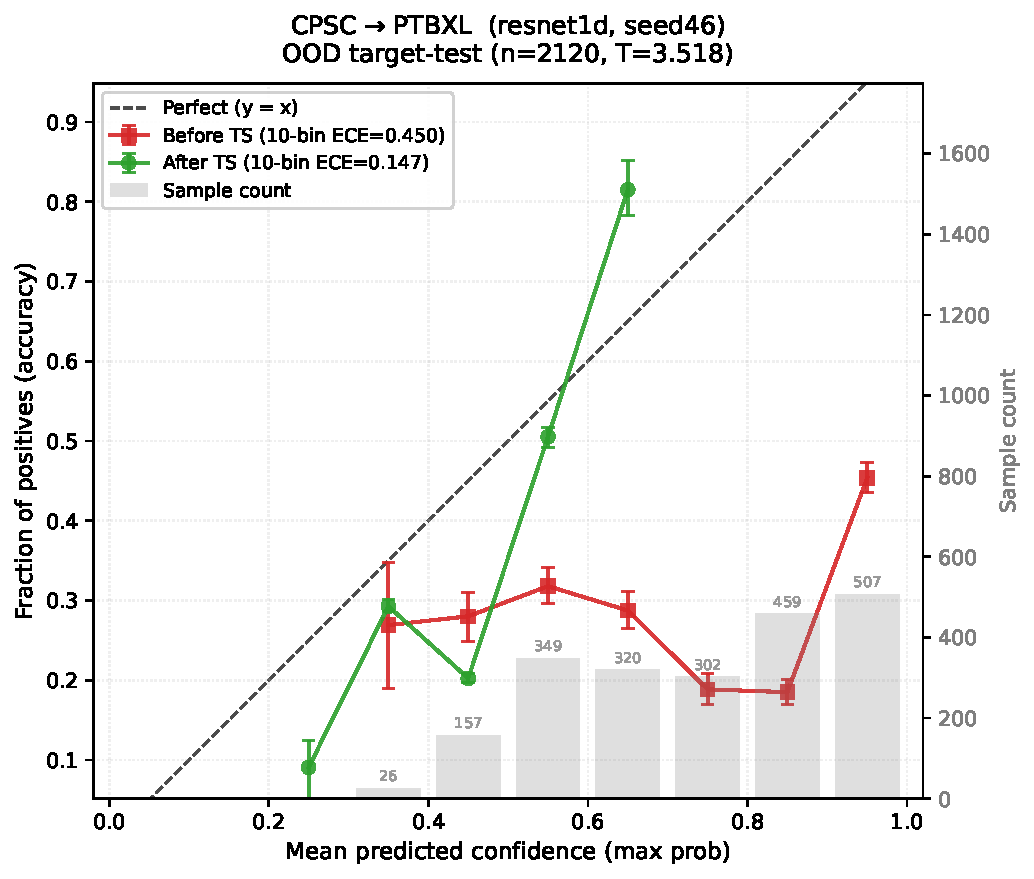
\includegraphics[width=0.45\textwidth]{figures/fig_reliability_supp_cpsc_ptbxl_resnet1d_seed46.pdf}
\caption{CPSC$\to$PTB-XL 可靠性图：ResNet1D 种子 45--46。}
\end{figure}

\begin{figure}[h]
\centering
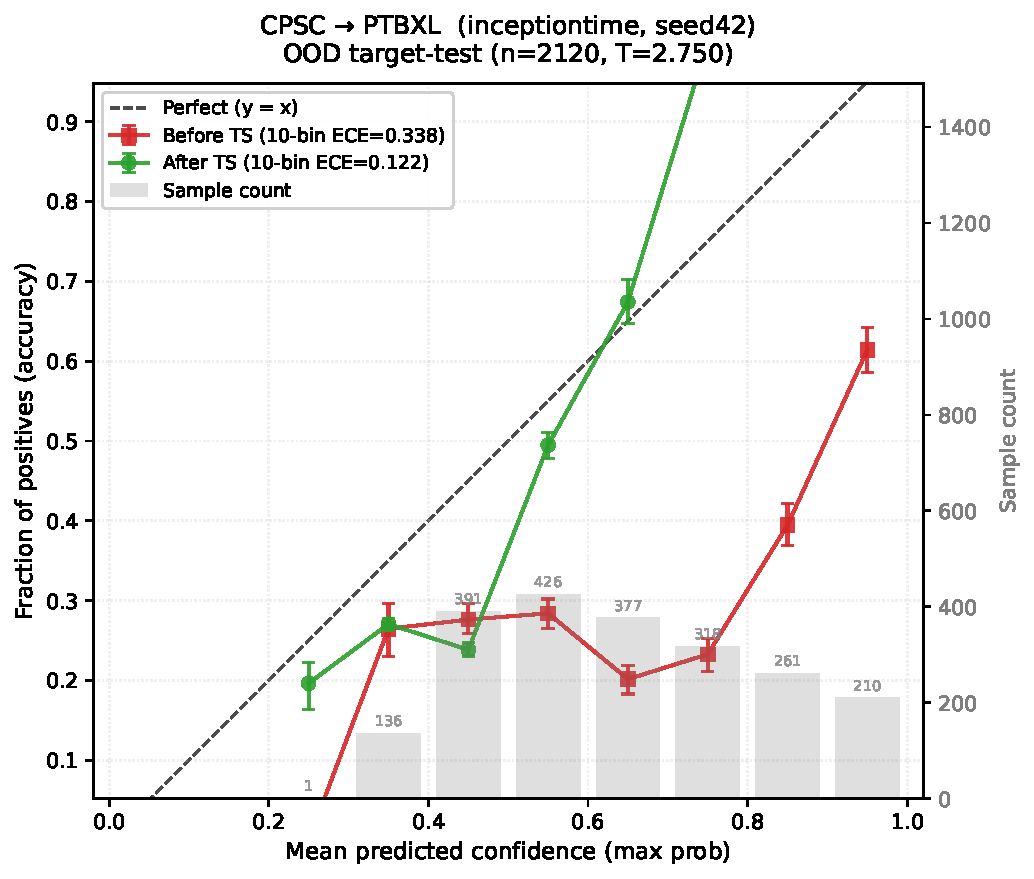
\includegraphics[width=0.32\textwidth]{figures/fig_reliability_supp_cpsc_ptbxl_inceptiontime_seed42.pdf}
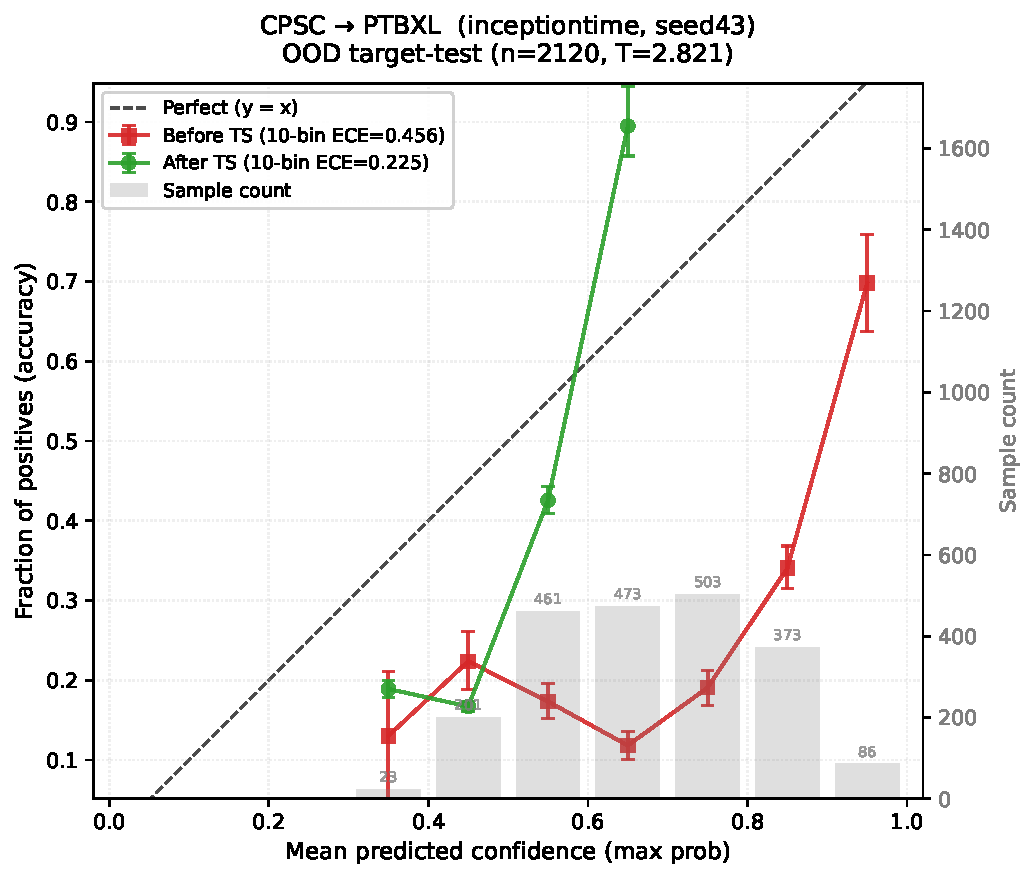
\includegraphics[width=0.32\textwidth]{figures/fig_reliability_supp_cpsc_ptbxl_inceptiontime_seed43.pdf}
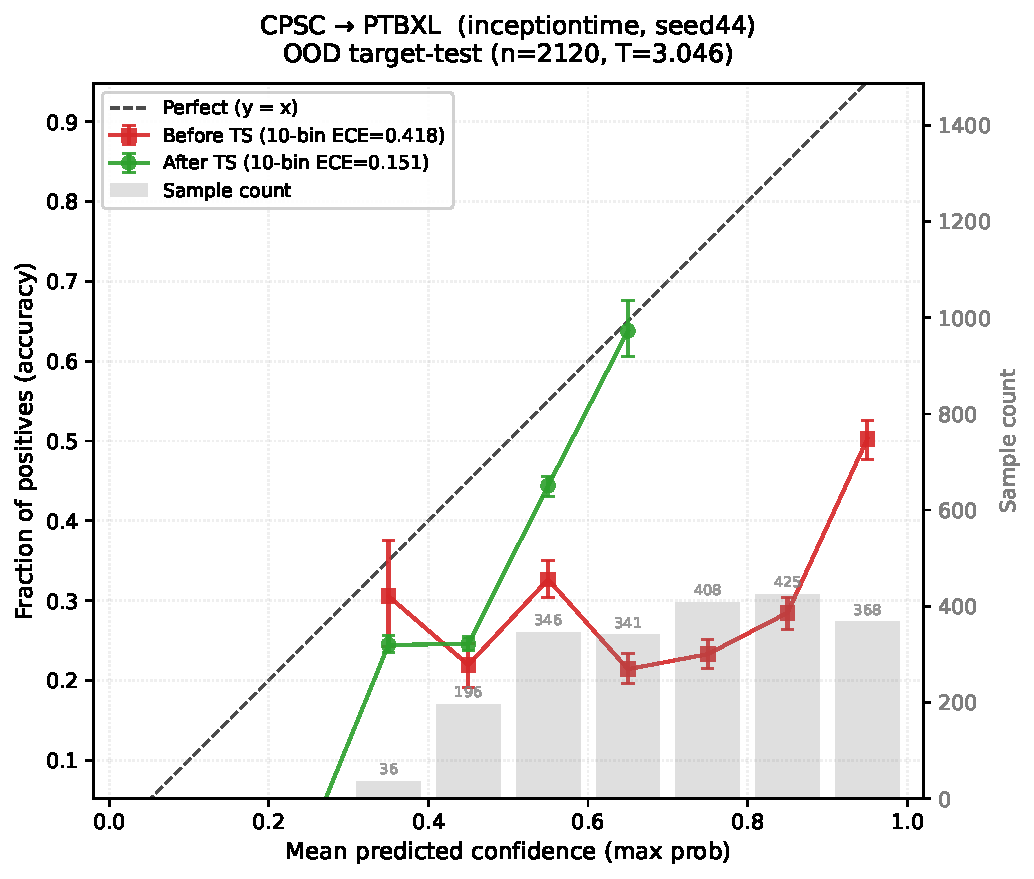
\includegraphics[width=0.32\textwidth]{figures/fig_reliability_supp_cpsc_ptbxl_inceptiontime_seed44.pdf}
\caption{CPSC$\to$PTB-XL 可靠性图：InceptionTime 种子 42--44。}
\end{figure}

\begin{figure}[h]
\centering
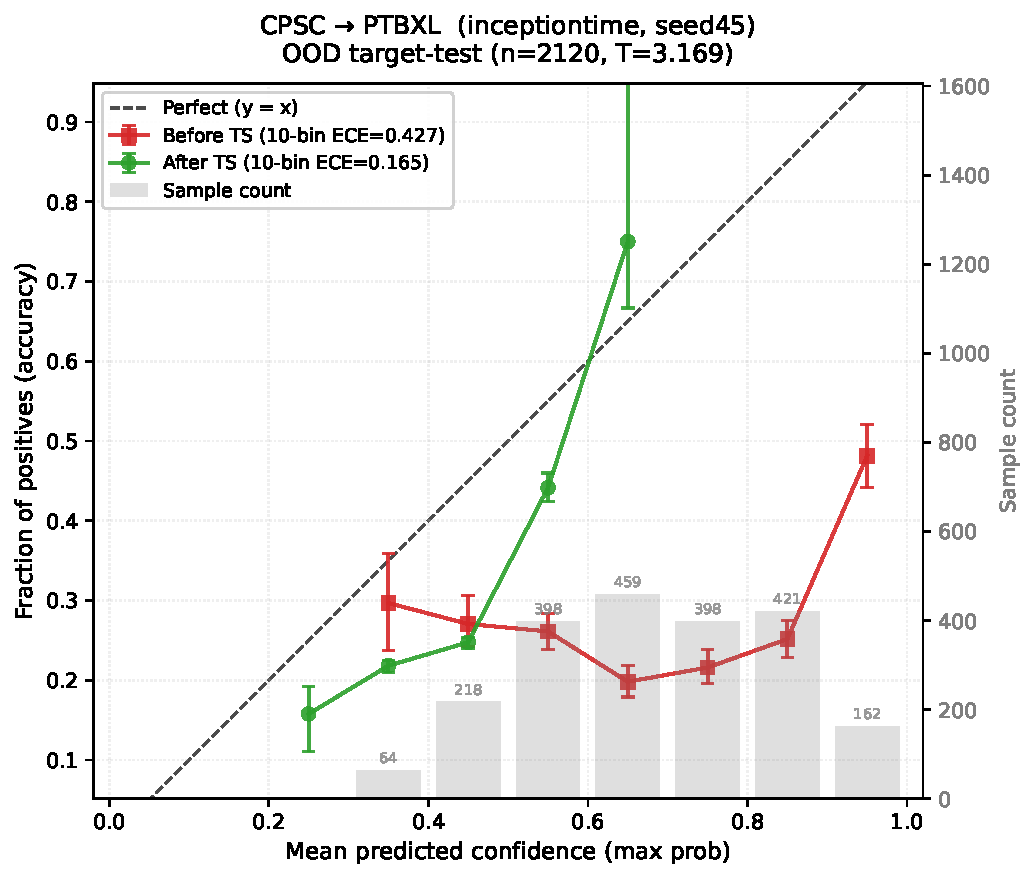
\includegraphics[width=0.45\textwidth]{figures/fig_reliability_supp_cpsc_ptbxl_inceptiontime_seed45.pdf}
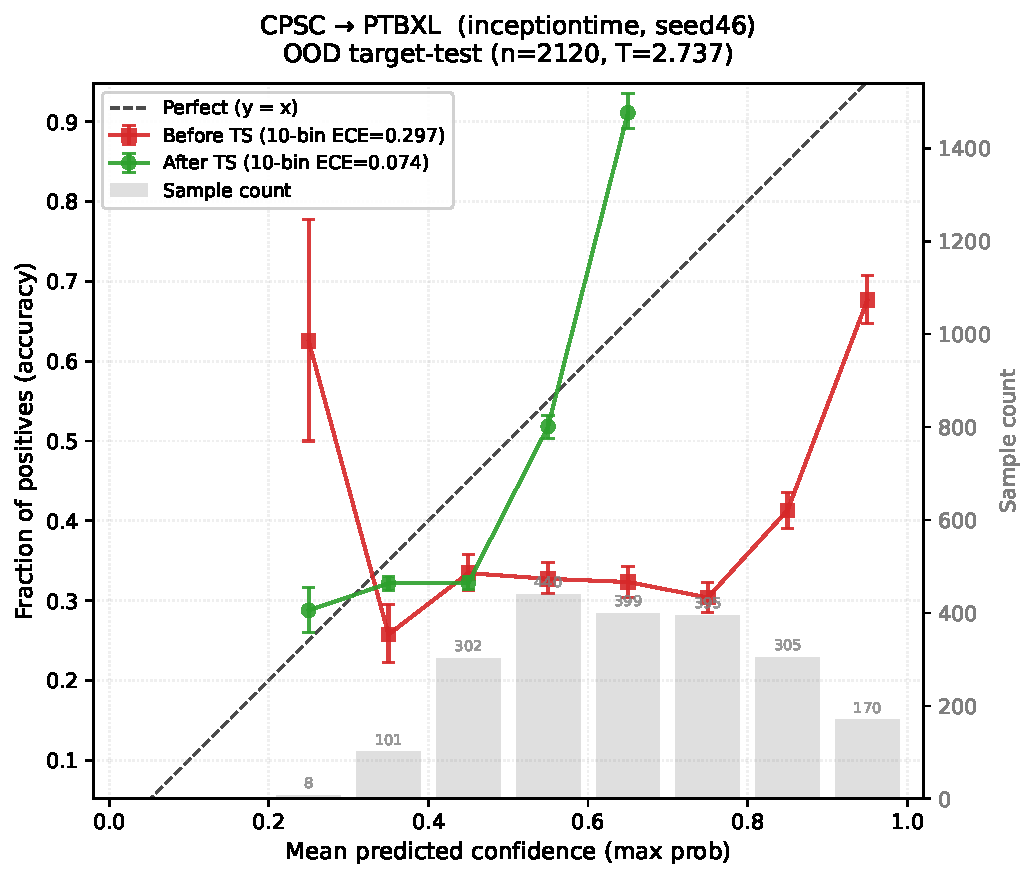
\includegraphics[width=0.45\textwidth]{figures/fig_reliability_supp_cpsc_ptbxl_inceptiontime_seed46.pdf}
\caption{CPSC$\to$PTB-XL 可靠性图：InceptionTime 种子 45--46。}
\end{figure}

\subsubsection*{S1.5.\ PTB-XL$\rightarrow$Chapman}

\begin{figure}[h]
\centering
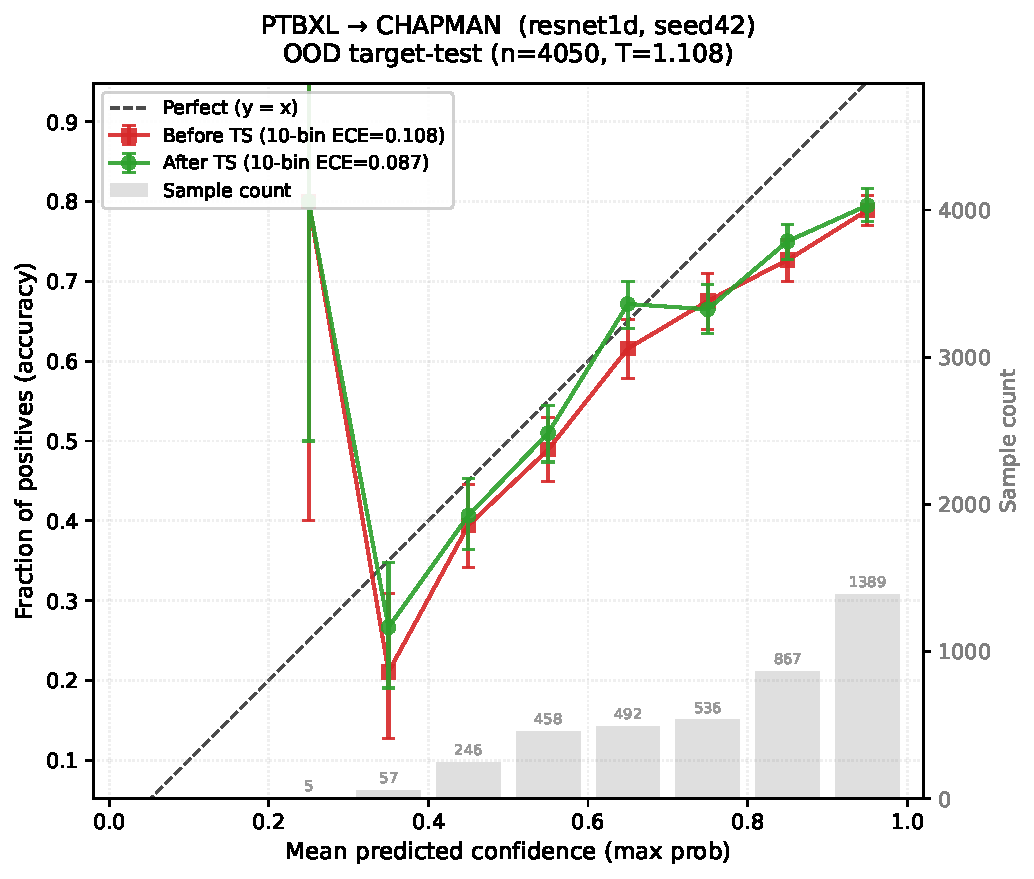
\includegraphics[width=0.32\textwidth]{figures/fig_reliability_supp_ptbxl_chapman_resnet1d_seed42.pdf}
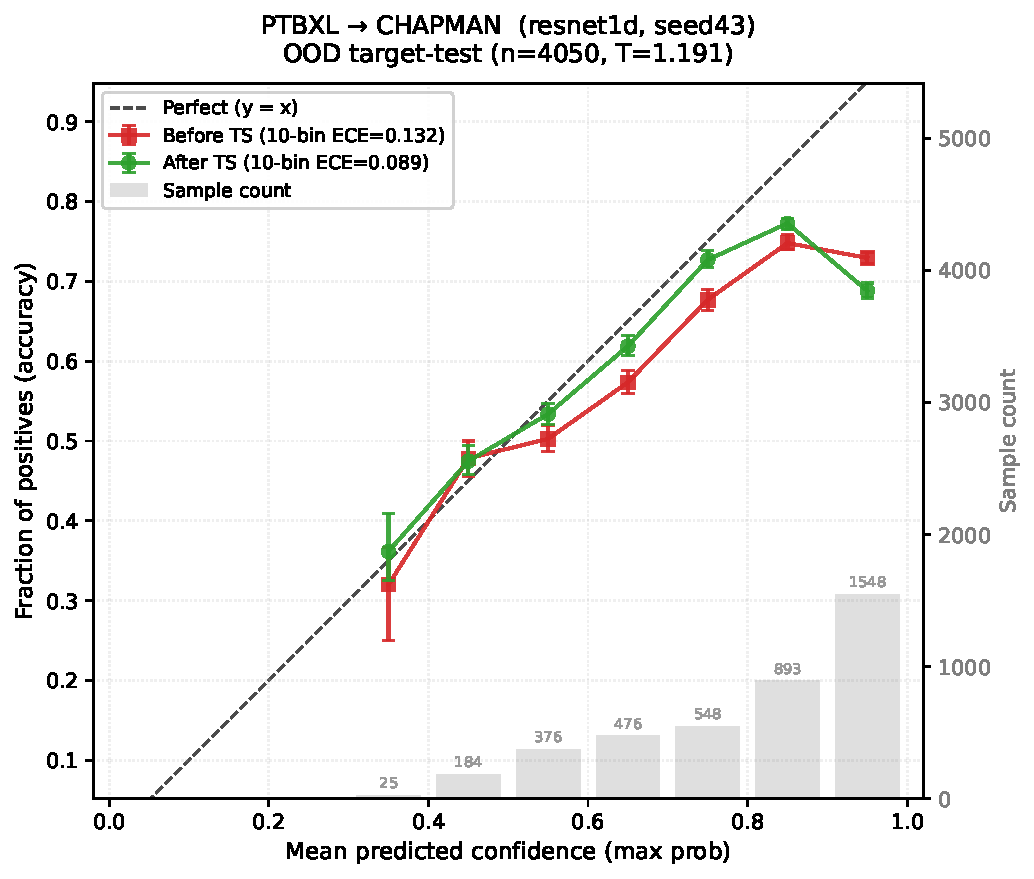
\includegraphics[width=0.32\textwidth]{figures/fig_reliability_supp_ptbxl_chapman_resnet1d_seed43.pdf}
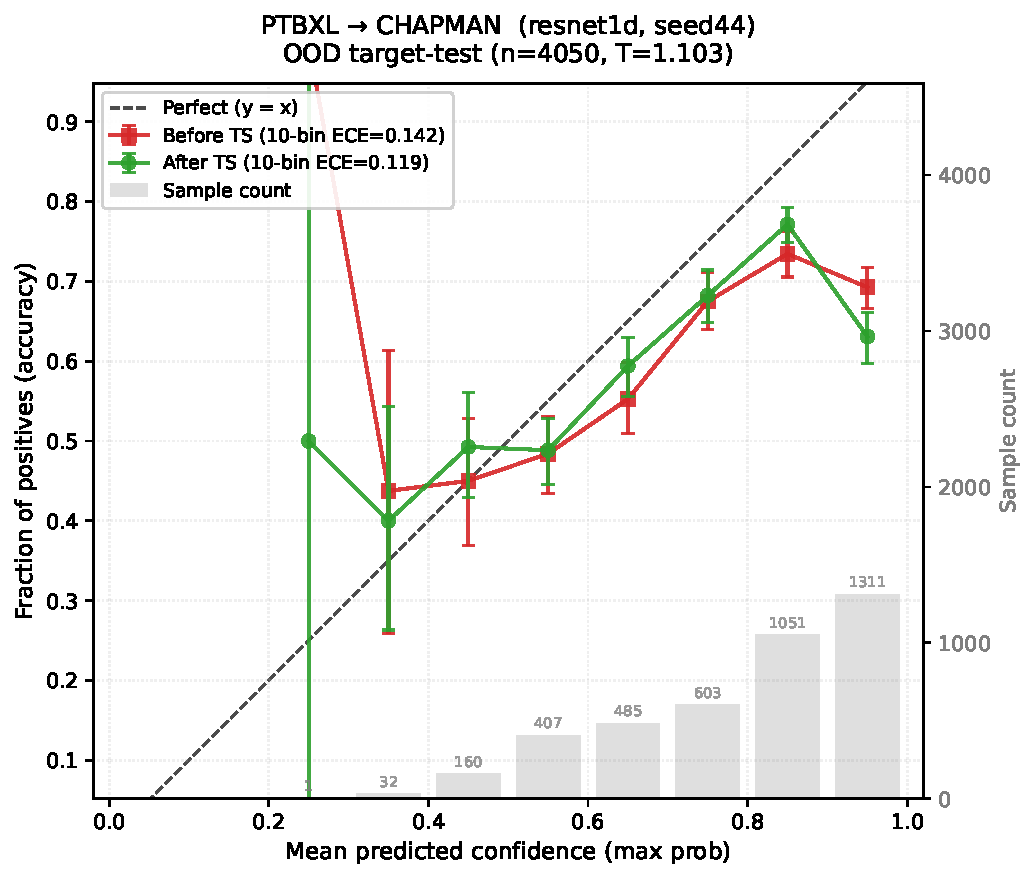
\includegraphics[width=0.32\textwidth]{figures/fig_reliability_supp_ptbxl_chapman_resnet1d_seed44.pdf}
\caption{PTB-XL$\to$Chapman 可靠性图：ResNet1D 种子 42--44。}
\end{figure}

\begin{figure}[h]
\centering
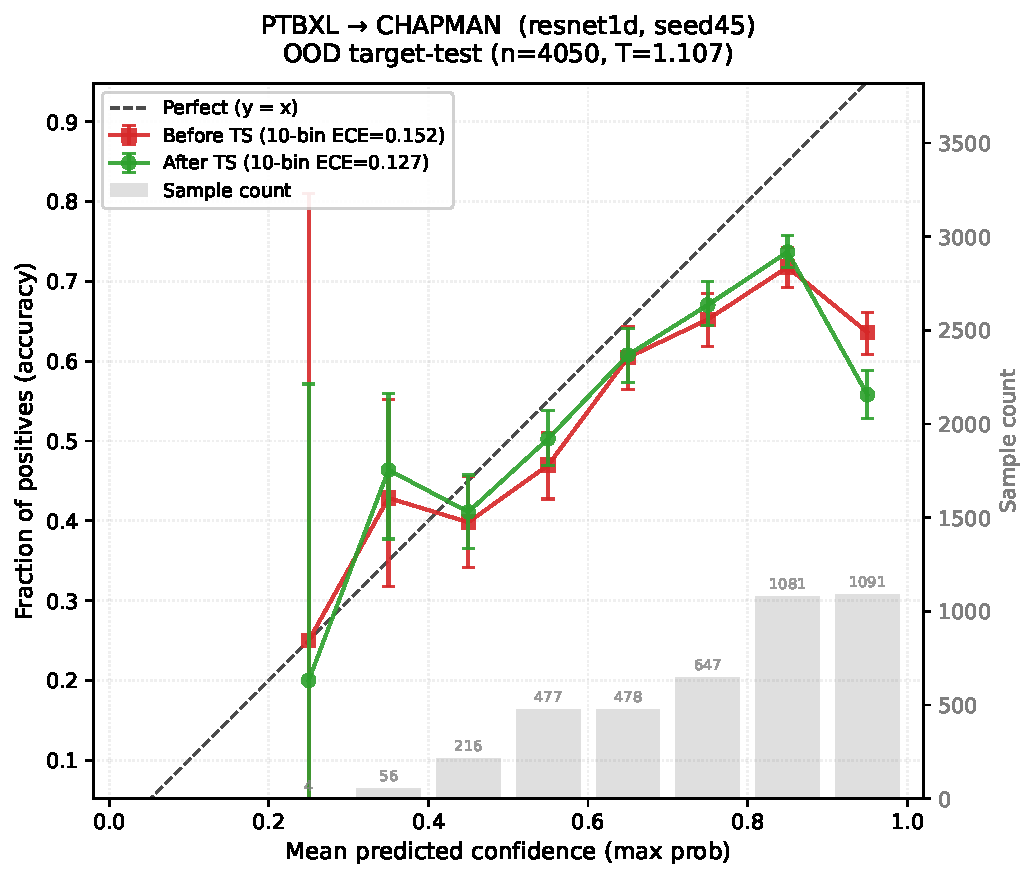
\includegraphics[width=0.45\textwidth]{figures/fig_reliability_supp_ptbxl_chapman_resnet1d_seed45.pdf}
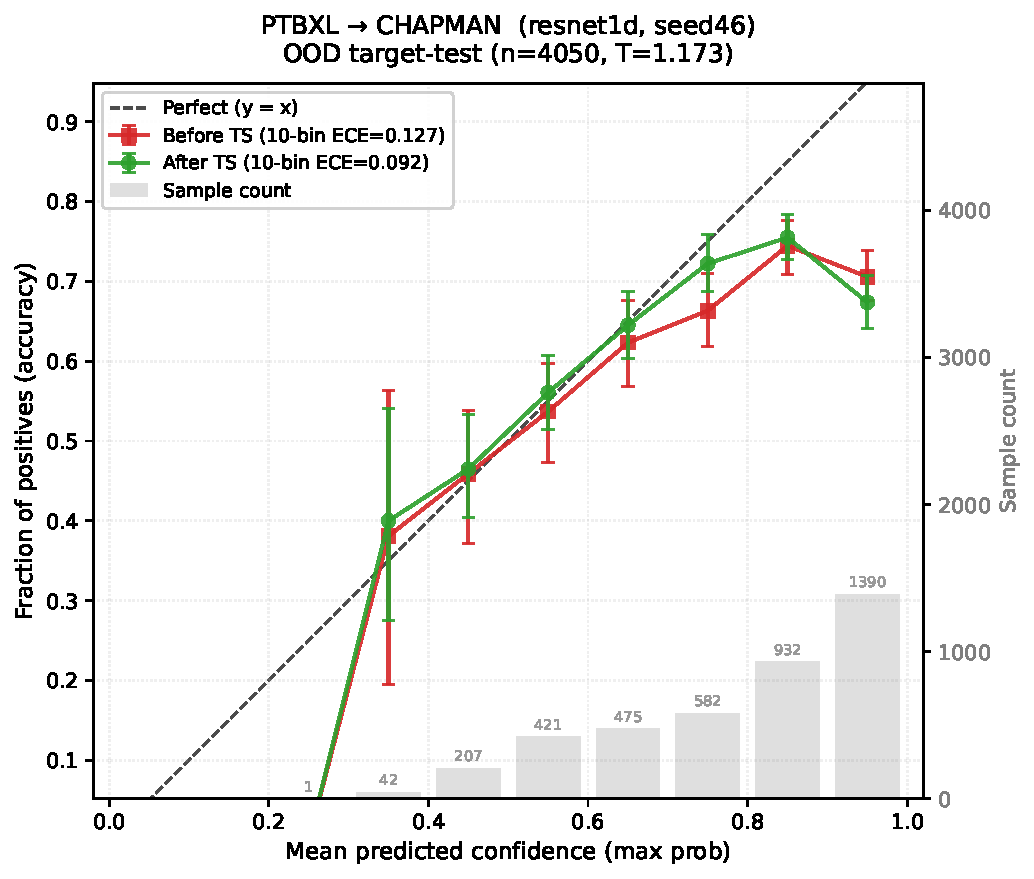
\includegraphics[width=0.45\textwidth]{figures/fig_reliability_supp_ptbxl_chapman_resnet1d_seed46.pdf}
\caption{PTB-XL$\to$Chapman 可靠性图：ResNet1D 种子 45--46。}
\end{figure}

\begin{figure}[h]
\centering
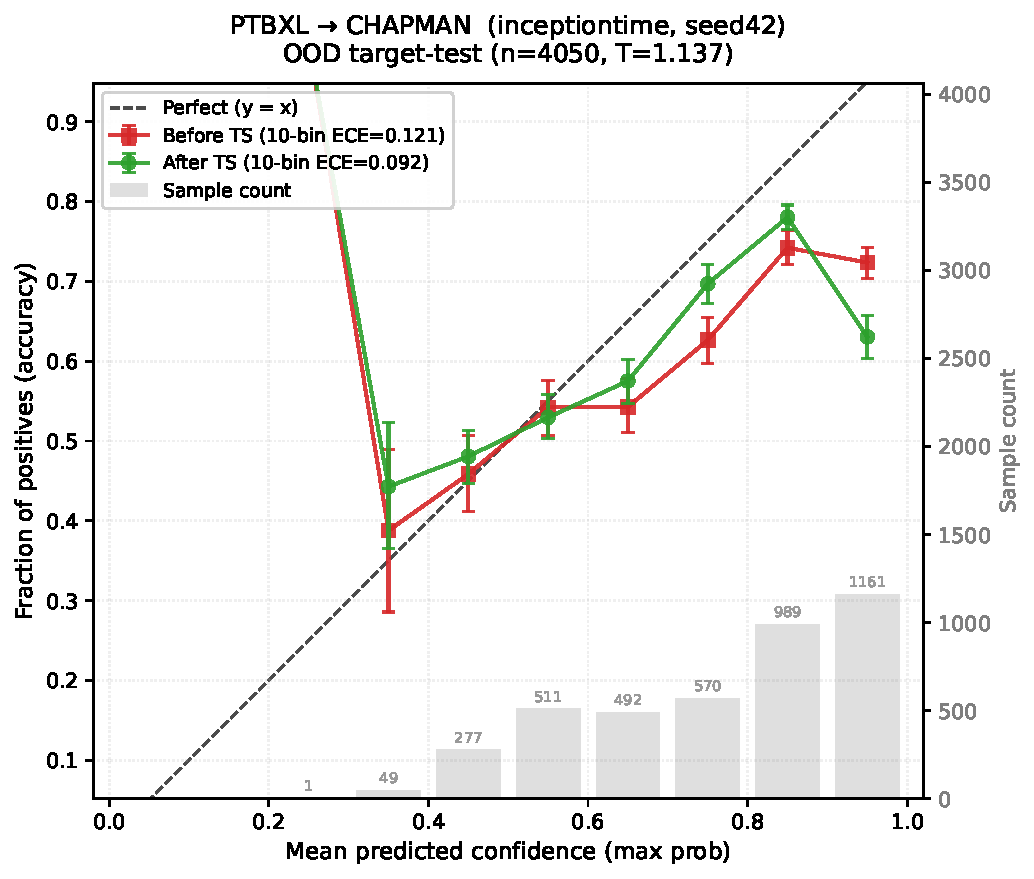
\includegraphics[width=0.32\textwidth]{figures/fig_reliability_supp_ptbxl_chapman_inceptiontime_seed42.pdf}
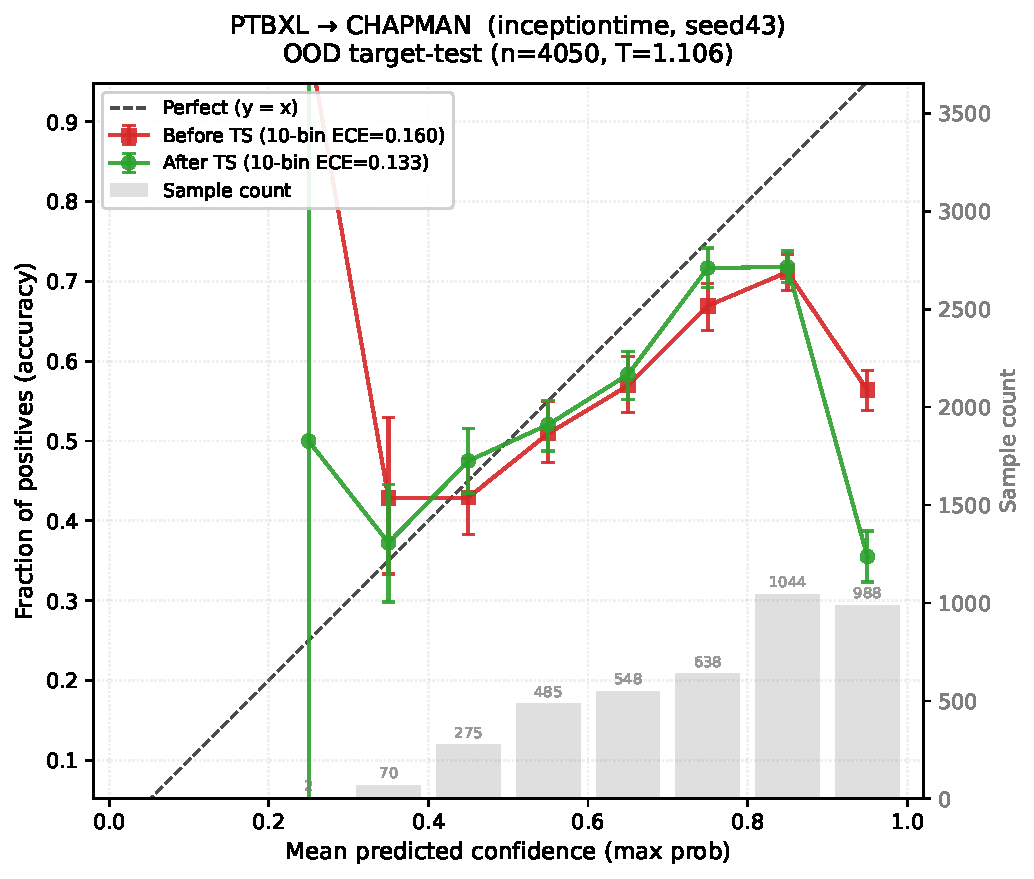
\includegraphics[width=0.32\textwidth]{figures/fig_reliability_supp_ptbxl_chapman_inceptiontime_seed43.pdf}
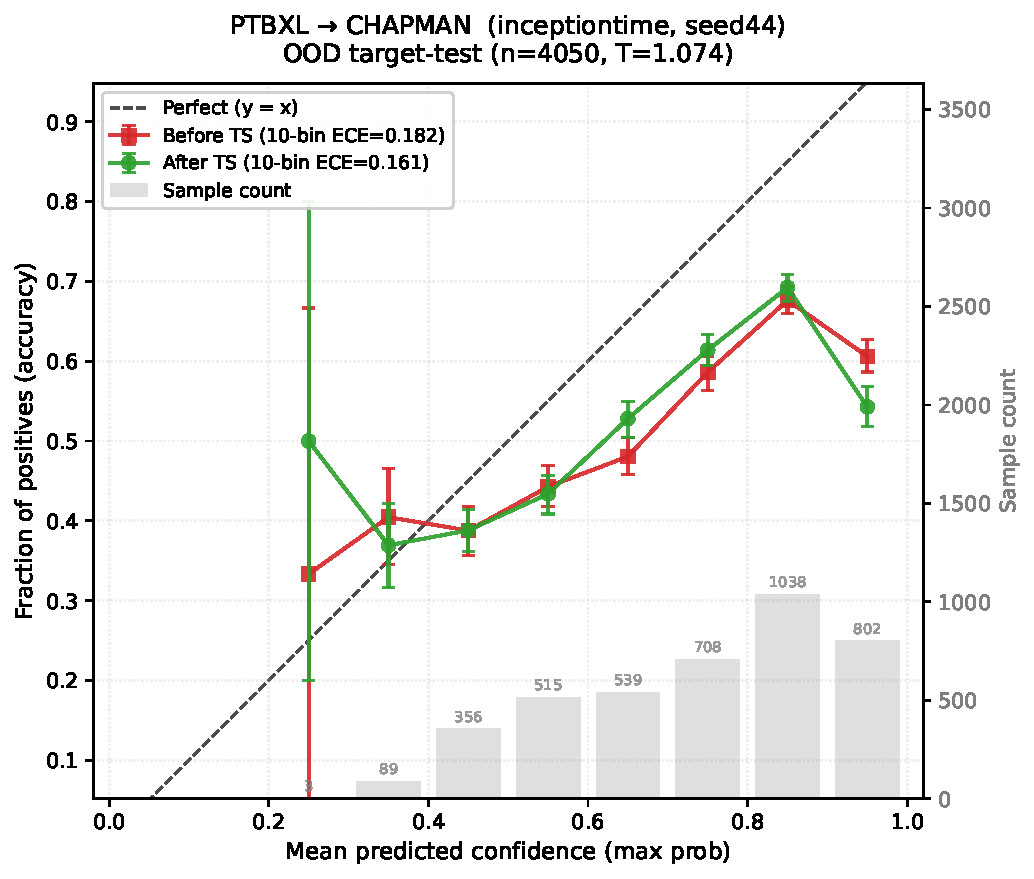
\includegraphics[width=0.32\textwidth]{figures/fig_reliability_supp_ptbxl_chapman_inceptiontime_seed44.pdf}
\caption{PTB-XL$\to$Chapman 可靠性图：InceptionTime 种子 42--44。}
\end{figure}

\begin{figure}[h]
\centering
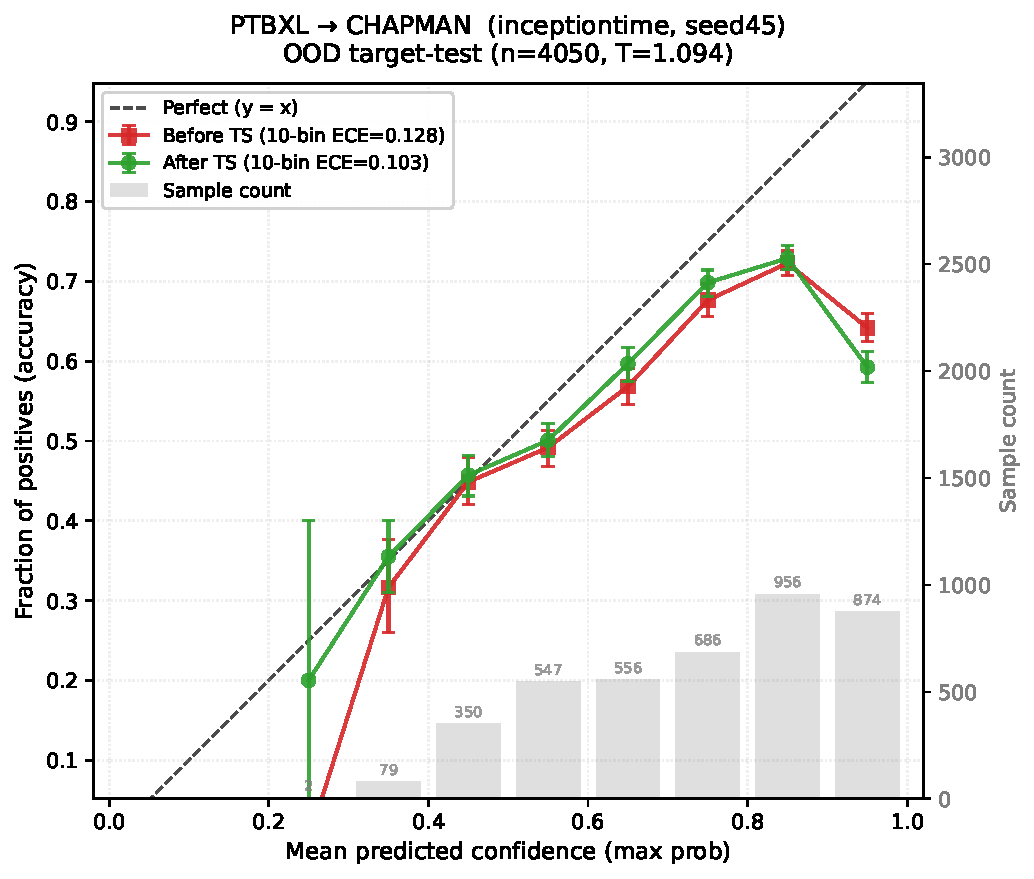
\includegraphics[width=0.45\textwidth]{figures/fig_reliability_supp_ptbxl_chapman_inceptiontime_seed45.pdf}
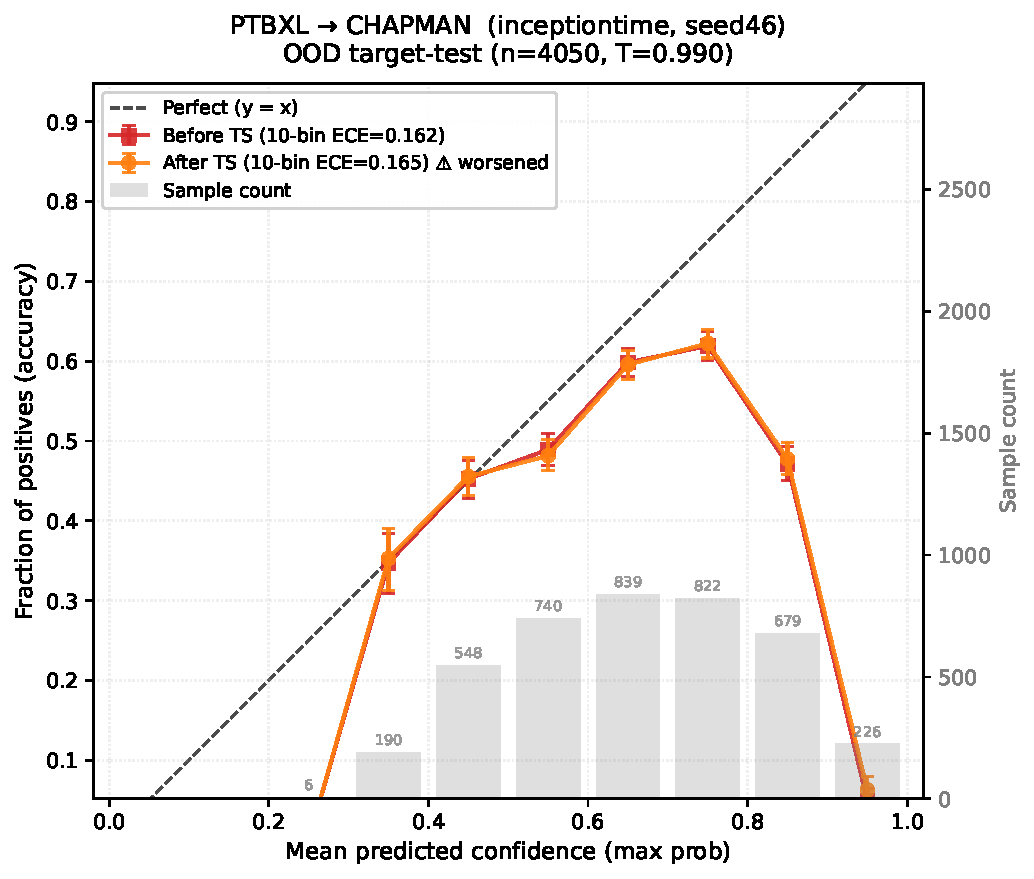
\includegraphics[width=0.45\textwidth]{figures/fig_reliability_supp_ptbxl_chapman_inceptiontime_seed46.pdf}
\caption{PTB-XL$\to$Chapman 可靠性图：InceptionTime 种子 45--46。}
\end{figure}

\subsubsection*{S1.6.\ PTB-XL$\rightarrow$CPSC}

\begin{figure}[h]
\centering
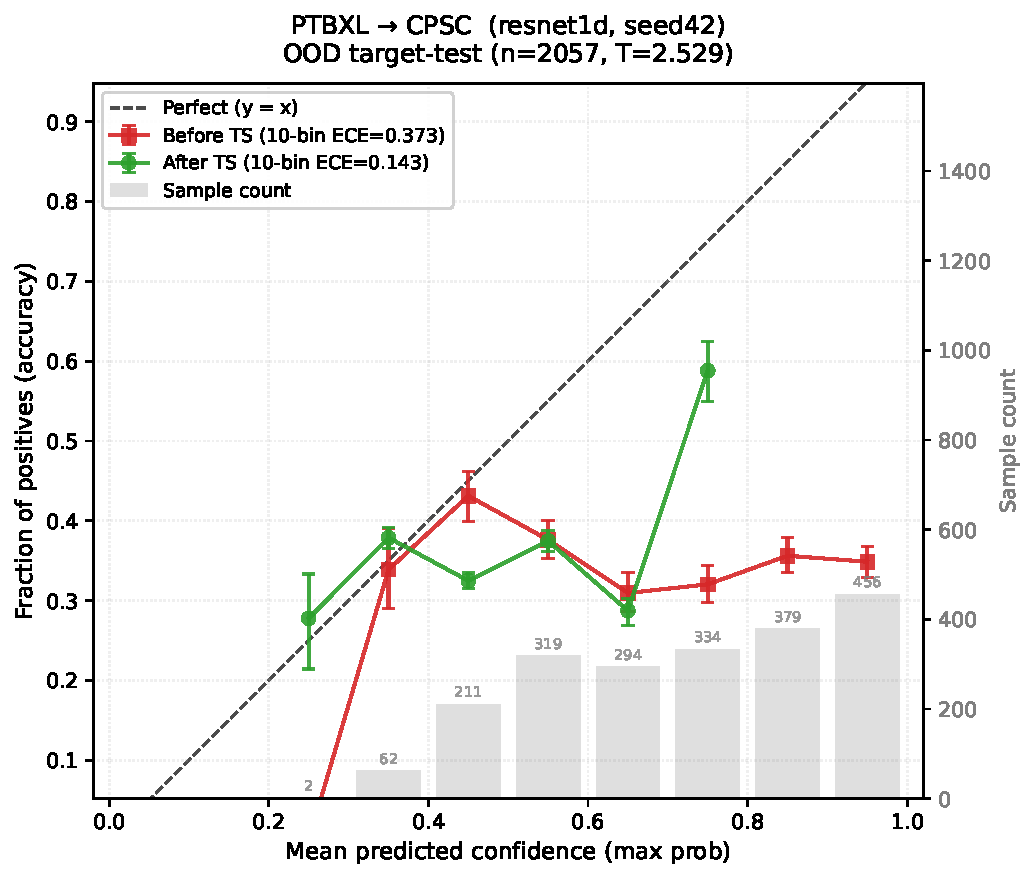
\includegraphics[width=0.32\textwidth]{figures/fig_reliability_supp_ptbxl_cpsc_resnet1d_seed42.pdf}
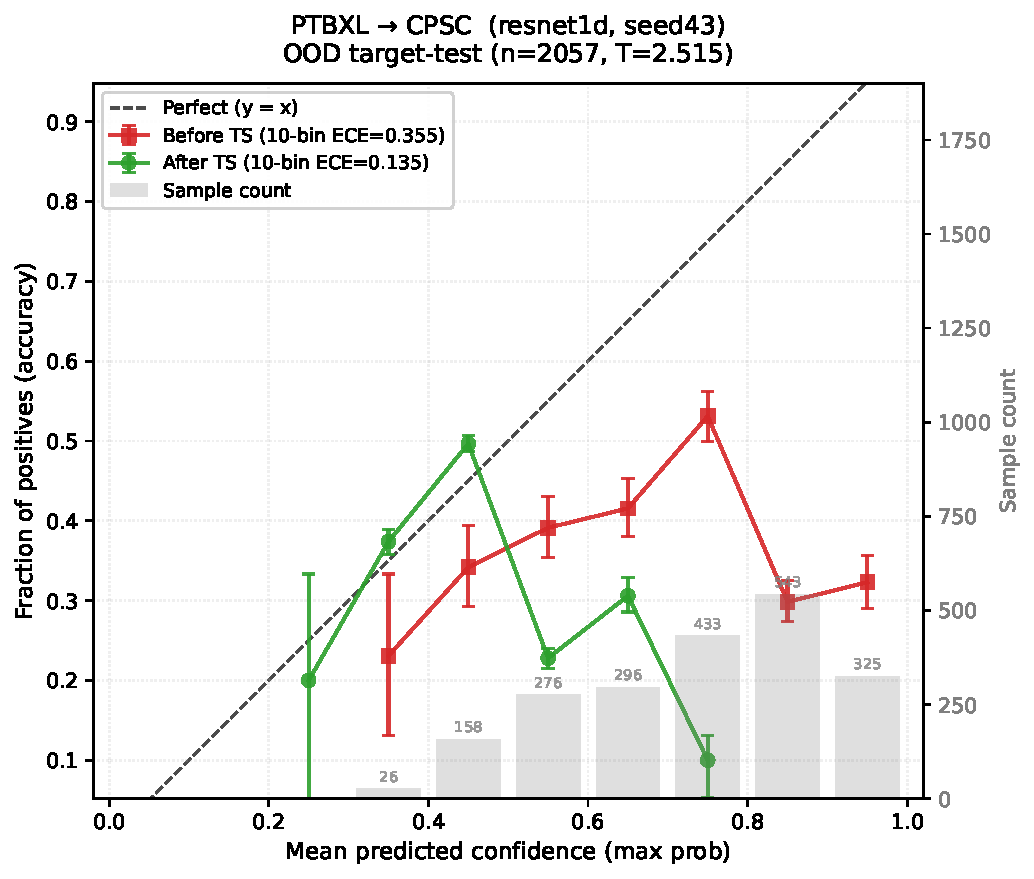
\includegraphics[width=0.32\textwidth]{figures/fig_reliability_supp_ptbxl_cpsc_resnet1d_seed43.pdf}
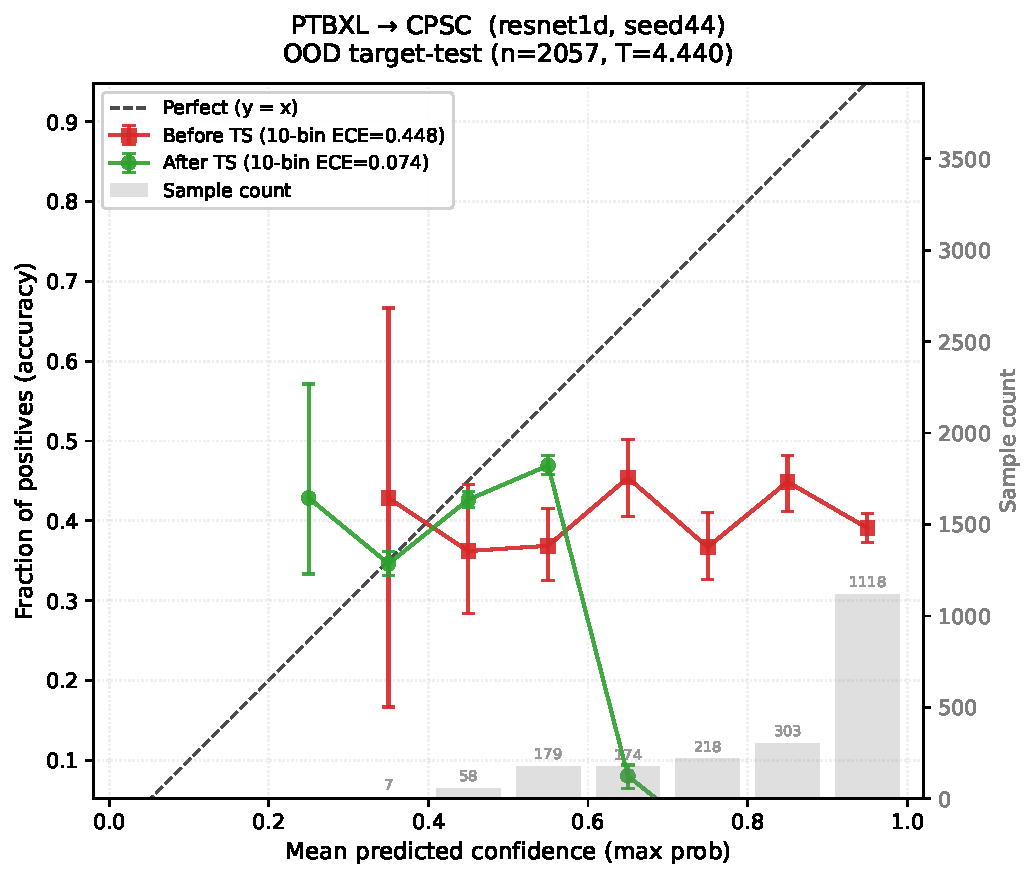
\includegraphics[width=0.32\textwidth]{figures/fig_reliability_supp_ptbxl_cpsc_resnet1d_seed44.pdf}
\caption{PTB-XL$\to$CPSC 可靠性图：ResNet1D 种子 42--44。}
\end{figure}

\begin{figure}[h]
\centering
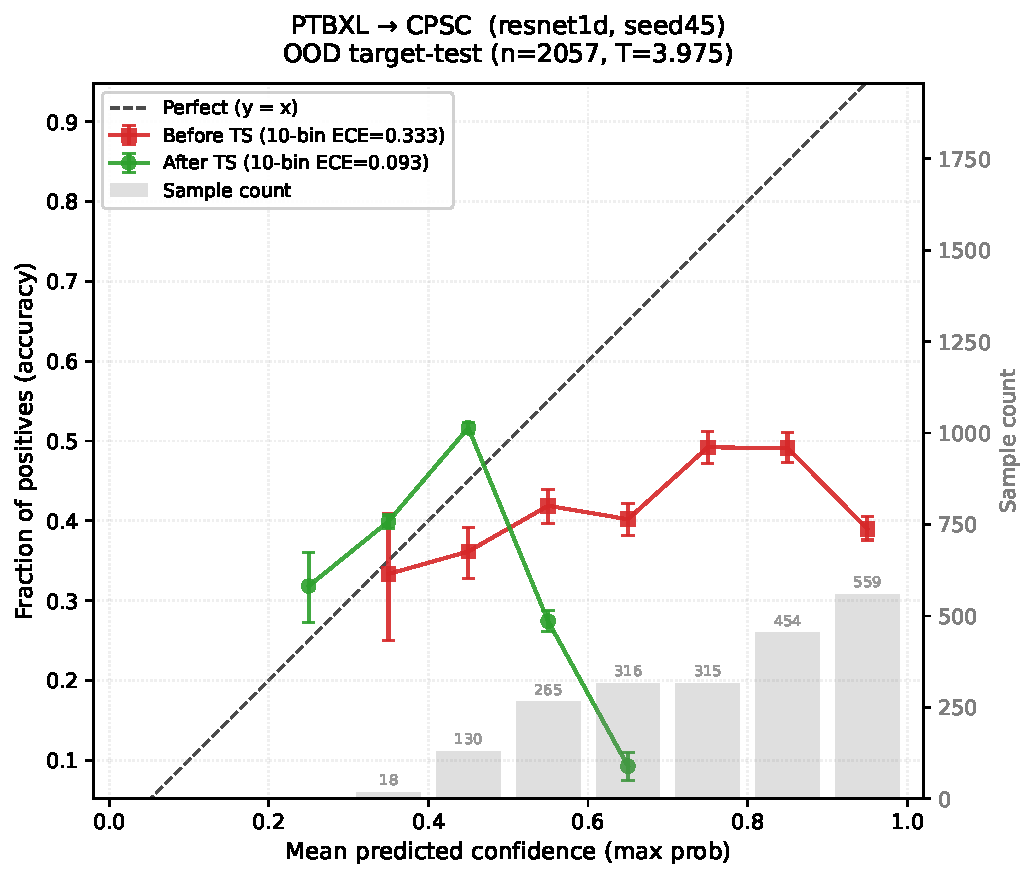
\includegraphics[width=0.45\textwidth]{figures/fig_reliability_supp_ptbxl_cpsc_resnet1d_seed45.pdf}
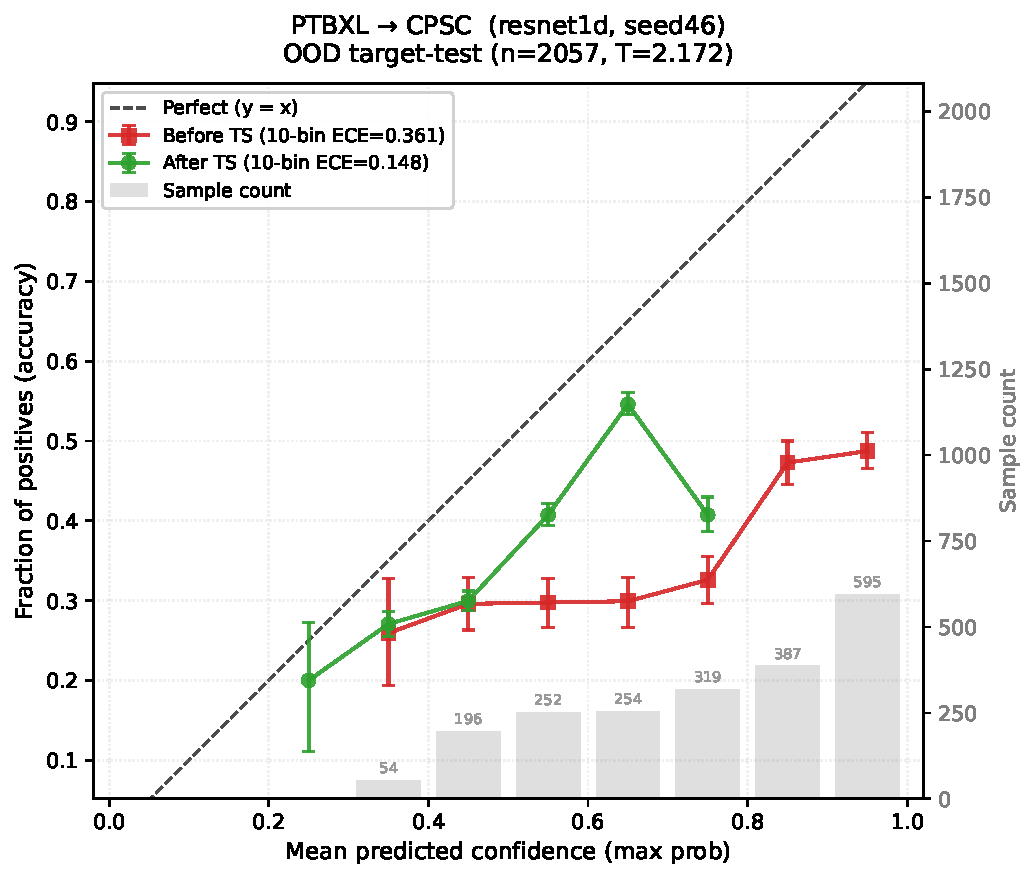
\includegraphics[width=0.45\textwidth]{figures/fig_reliability_supp_ptbxl_cpsc_resnet1d_seed46.pdf}
\caption{PTB-XL$\to$CPSC 可靠性图：ResNet1D 种子 45--46。}
\end{figure}

\begin{figure}[h]
\centering
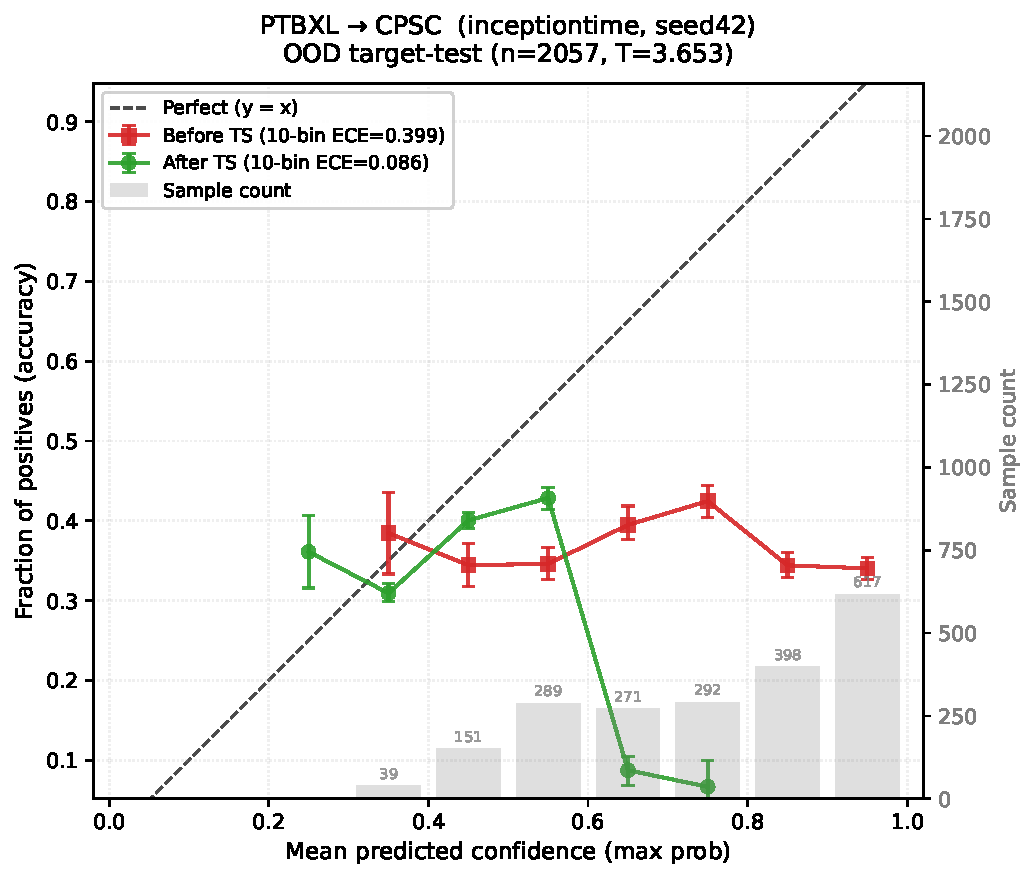
\includegraphics[width=0.32\textwidth]{figures/fig_reliability_supp_ptbxl_cpsc_inceptiontime_seed42.pdf}
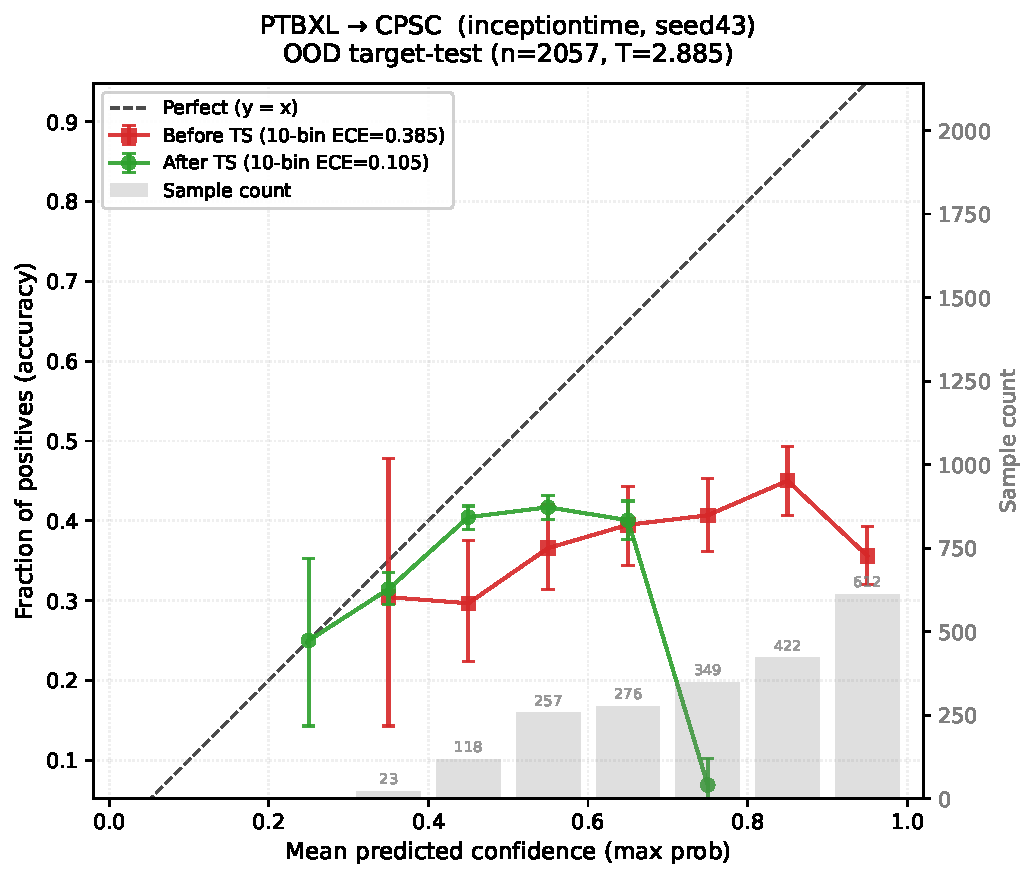
\includegraphics[width=0.32\textwidth]{figures/fig_reliability_supp_ptbxl_cpsc_inceptiontime_seed43.pdf}
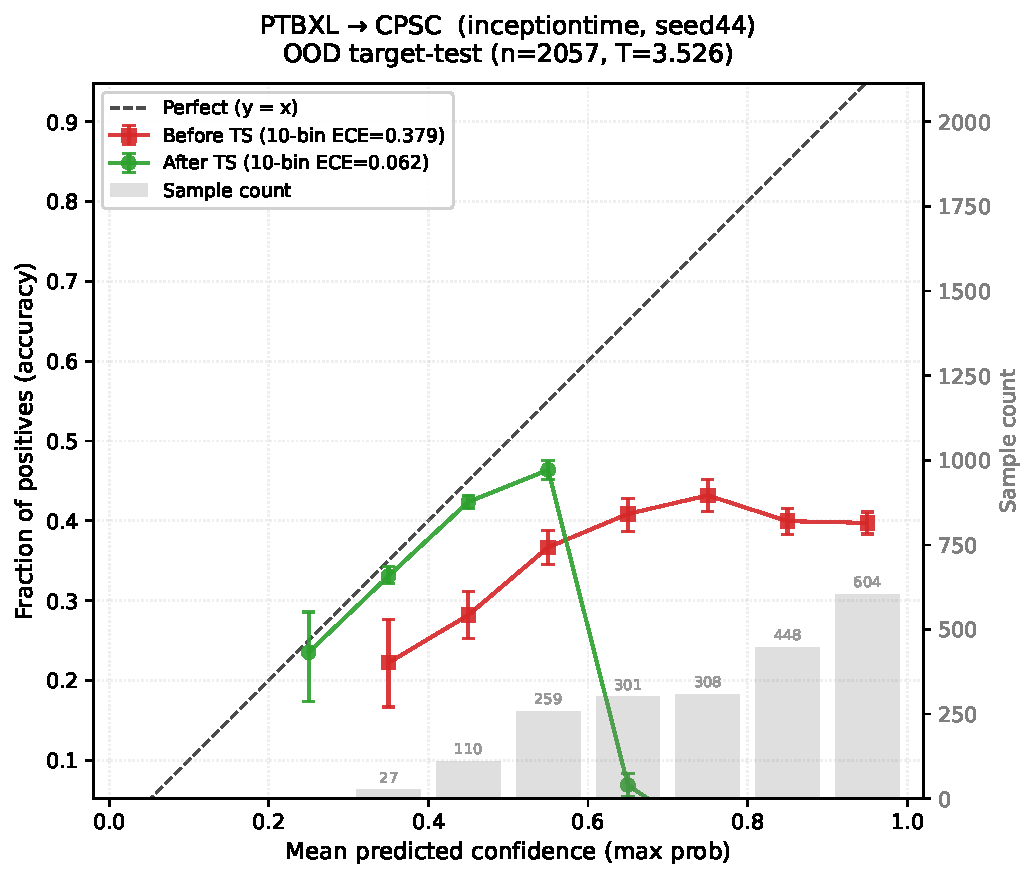
\includegraphics[width=0.32\textwidth]{figures/fig_reliability_supp_ptbxl_cpsc_inceptiontime_seed44.pdf}
\caption{PTB-XL$\to$CPSC 可靠性图：InceptionTime 种子 42--44。}
\end{figure}

\begin{figure}[h]
\centering
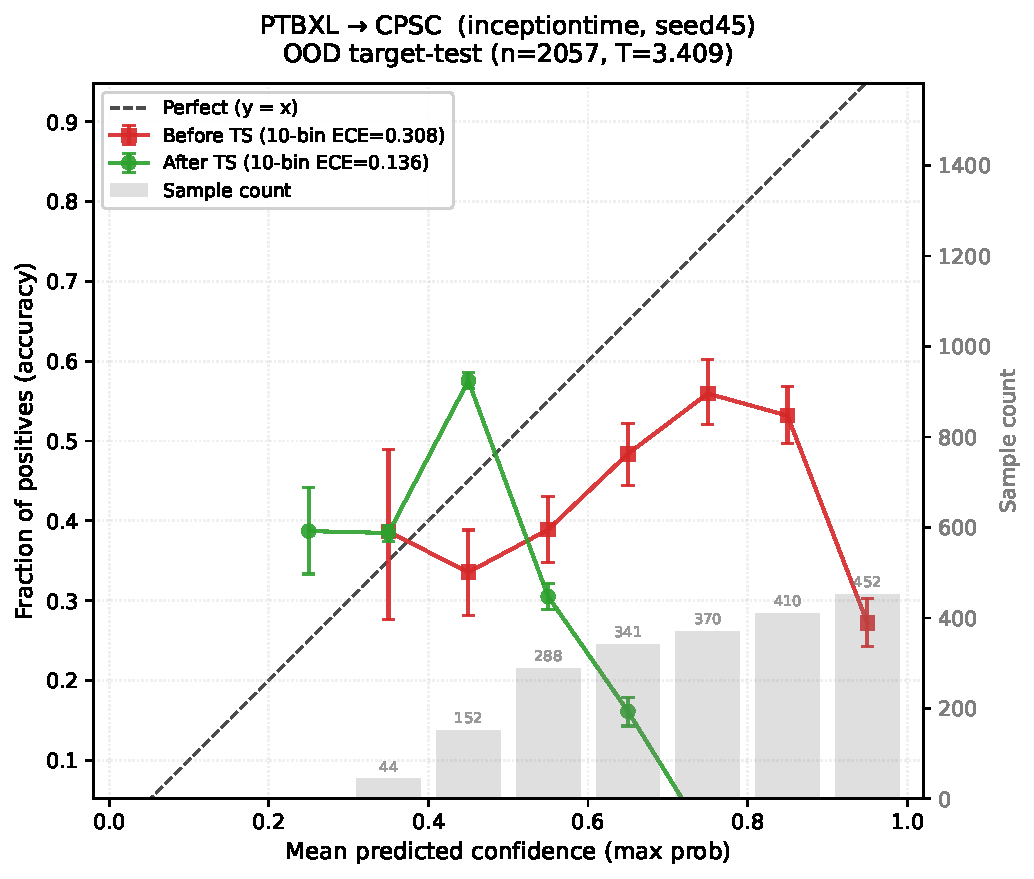
\includegraphics[width=0.45\textwidth]{figures/fig_reliability_supp_ptbxl_cpsc_inceptiontime_seed45.pdf}
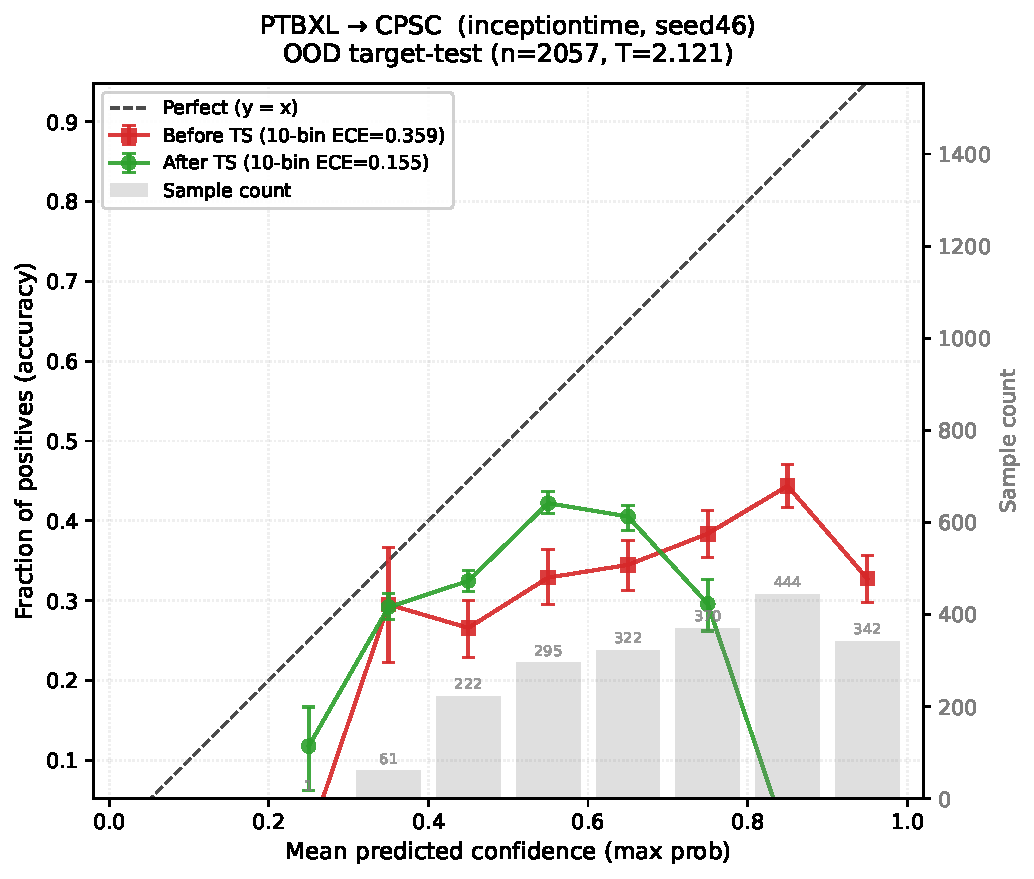
\includegraphics[width=0.45\textwidth]{figures/fig_reliability_supp_ptbxl_cpsc_inceptiontime_seed46.pdf}
\caption{PTB-XL$\to$CPSC 可靠性图：InceptionTime 种子 45--46。}
\end{figure}

\subsection*{S2.\ 其他补充材料}
\label{sec:supp-additional}
\begin{itemize}
    \item \textbf{逐实验结果文件}：全部 60 个种子实验的完整 JSON 结果
    （\texttt{checkpoints/transfer/**/}\allowbreak\texttt{transfer\_result.json}）
    和 CSV 汇总（\texttt{results/*.csv}）。
    \item \textbf{预注册协议}：修订版 A1 全文
    （\texttt{docs/PROTOCOL\_AMENDMENT\_A1\_}\allowbreak\texttt{PREREG\_RELOCATION.md}）
    和哈希清单（\texttt{docs/osf\_archive\_manifest.json}）。
    \item \textbf{NCV 实验数据}：包含净临床价值实验（Section~\ref{sec:ncv_methods}）
    所用 \texttt{ncv\_id} 和 \texttt{ncv\_ood} 列的 E3 CSV 文件。
    \item \textbf{Shapley 分解单元}：用于 $n=20{,}000$ 处 Shapley 归因分析的
    27 单元验证表。
    \item \textbf{BCa 置信区间重算清单}：整个 $6 \times 2 \times 5 \times 8$
    网格的完整 BCa 自助法（$B=10{,}000$）置信区间结果，存储于每个
    \texttt{transfer\_result.json} 的 \texttt{methods.ts.meta} 字段中。
\end{itemize}


% ============================================================================
\section*{参考文献}
% Bibliography — 中文翻译（保留原始 \bibitem 格式，每条后附中文标题注释）
% 对应 main.tex 第 2223--2358 行 \begin{thebibliography}...\end{thebibliography}
\begin{thebibliography}{99}
\raggedright
% ============================================================================
\bibitem{ovadia2019calibration} Y.~Ovadia, E.~Fertig, J.~Ren, Z.~Nado,
D.~Sculley, S.~Nowozin, J.~Dillon, B.~Lakshminarayanan, J.~Snoek,
``Can you trust your model's uncertainty? Evaluating predictive
uncertainty under dataset shift,'' \emph{NeurIPS}, 2019.
arXiv:1906.02530.
% 中文标题：你能信任模型的不确定性吗？数据集偏移下的预测不确定性评估
\bibitem{guo2017calibration} C.~Guo, G.~Pleiss, Y.~Sun, K.~Weinberger,
``On calibration of modern neural networks,'' \emph{ICML}, PMLR
70:1321--1330, 2017. arXiv:1706.04599.
% 中文标题：论现代神经网络的校准
\bibitem{wagner2020ptbxl} P.~Wagner, N.~Strodthoff, R.-D.~Bousseljot,
et al., ``PTB-XL, a large publicly available electrocardiography
dataset,'' \emph{Scientific Data}, 7:154, 2020.
doi:10.1038/s41597-020-0495-6.
% 中文标题：PTB-XL，一个大规模公开可获取的心电数据集
\bibitem{zheng2022ecgarrhythmia} J.~Zheng, J.~Guo, H.~Chu,
``A large scale 12-lead electrocardiogram database for arrhythmia
study (Chapman-Shaoxing e-cardiology),'' version 1.0.0,
\emph{PhysioNet}, 2022. doi:10.13026/wgex-er52.
% 中文标题：用于心律失常研究的大规模 12 导联心电图数据库（Chapman-Shaoxing 电子心脏病学）
\bibitem{goldberger2000} A.~L. Goldberger et al., ``PhysioBank,
PhysioToolkit, and PhysioNet: components of a new research resource
for complex physiologic signals,'' \emph{Circulation},
101(23):e215--e220, 2000.
% 中文标题：PhysioBank、PhysioToolkit 与 PhysioNet：面向复杂生理信号新研究资源的组成部分
\bibitem{nixon2019} J.~Nixon, M.~W. Dusenberry, L.~Zhang, et al.,
``Measuring calibration in deep learning,'' \emph{CVPR Workshops},
pp.~38--41, 2019. arXiv:1904.01685.
% 中文标题：深度学习中的校准度量
\bibitem{kull2019dirichlet} M.~Kull, M.~Perello-Nieto, M.~Kangse,
T.~S.~Filho, P.~Song, P.~Flach, ``Beyond temperature scaling:
obtaining well-calibrated multi-class probabilities with Dirichlet
calibration,'' \emph{NeurIPS}, 2019. arXiv:1910.12656.
% 中文标题：超越温度缩放：用 Dirichlet 校准获取良好校准的多类概率
\bibitem{alexandari2020} A.~Alexandari, A.~Kundaje, A.~Shrikumar,
``Maximum likelihood with bias-corrected calibration is hard-to-beat
at label shift adaptation,'' \emph{ICML}, PMLR 119:222--232, 2020.
arXiv:1901.06852.
% 中文标题：带偏差校正校准的最大似然在标签偏移适应中难以被超越
\bibitem{lipton2018bbs} Z.~Lipton, Y.-X.~Wang, A.~Smola,
``Detecting and correcting for label shift with black box
predictors,'' \emph{ICML}, PMLR 80:1944--1953, 2018.
arXiv:1802.03916.
% 中文标题：用黑盒预测器检测和校正标签偏移
\bibitem{barandas2023} M.~Barandas, L.~Famiglini, A.~Campagner,
D.~Folgado, R.~Sim\~ao, F.~Cabitza, H.~Gamboa, ``Evaluation of
uncertainty quantification methods in multi-label classification: a
case study with automatic diagnosis of electrocardiogram,''
\emph{Information Fusion}, 101:101978, 2024.
doi:10.1016/j.inffus.2023.101978.
% 中文标题：多标签分类中不确定性量化方法的评估：以心电图自动诊断为案例研究
\bibitem{zhang2022} J.~F.~Vranken et al., ``Uncertainty estimation for
deep learning-based automated analysis of 12-lead
electrocardiograms,'' \emph{European Heart Journal -- Digital Health},
2(3):423--434, 2021. doi:10.1093/ehjdh/ztab045.
% 中文标题：基于深度学习的 12 导联心电图自动分析的不确定性估计
\bibitem{reyna2022} M.~Reyna, N.~Strodthoff, P.~Wagner, et al.,
``Issues in the automated classification of multilead ECGs using
heterogeneous labels and populations,'' \emph{Physiological
Measurement}, 43(8):084001, 2022. doi:10.1088/1361-6579/ac79fd.
% 中文标题：使用异构标签和人群进行多导联心电图自动分类中的若干问题
\bibitem{efron1987bca} B.~Efron, ``Better bootstrap confidence
intervals,'' \emph{Journal of the American Statistical Association},
82(397):171--185, 1987. doi:10.1080/01621459.1987.10478410.
% 中文标题：更好的自助法置信区间
\bibitem{vancalster2016} B.~Van Calster, D.~J.~Steyerberg,
S.~Collins, R.~D.~Riley, E.~W.~Steyer, ``A calibration hierarchy for
risk models was defined: from utopia to empirical data,''
\emph{Journal of Clinical Epidemiology}, 74:167--176, 2016.
doi:10.1016/j.jclinepi.2015.12.005.
% 中文标题：风险模型校准层级的定义：从乌托邦到经验数据
\bibitem{vancalster2019} B.~Van Calster, D.~J.~McLernon,
M.~van~Smeden, L.~Wynants, G.~S.~Collins, ``Calibration: the Achilles
heel of predictive analytics,'' \emph{BMC Medicine}, 17:230, 2019.
doi:10.1186/s12916-019-1466-7.
% 中文标题：校准：预测分析的阿喀琉斯之踵
\bibitem{kumar2019} A.~Kumar, P.~Liang, T.~Ma, ``Verified uncertainty
calibration,'' \emph{NeurIPS}, 2019. arXiv:1909.10155.
% 中文标题：经验证的不确定性校准
\bibitem{strodthoff2021} N.~Strodthoff, P.~Wagner, T.~Schaeffter,
W.~Samek, ``Deep learning for ECG analysis: benchmarks and insights
from PTB-XL,'' \emph{IEEE Journal of Biomedical and Health
Informatics}, 25(5):1519--1528, 2021.
doi:10.1109/JBHI.2020.3022989.
% 中文标题：用于心电图分析的深度学习：来自 PTB-XL 的基准与见解
\bibitem{physiolmeas2026} M.~Haekal, S.~N.~Khotimah,
G.~R.~F.~Suwandi, F.~Haryanto, ``RR-interval-based atrial fibrillation
detection and burden estimation: cross-dataset validation and
calibration-aware probability analysis,'' \emph{Physiological
Measurement}, 2026. doi:10.1088/1361-6579/ae99aa.
% 中文标题：基于 RR 间期的心房颤动检测与负荷估计：跨数据集验证与校准感知概率分析
\bibitem{medrxiv2026} K.~Patel, P.~Beedala, ``Calibration drift under
cross-institutional deployment: an external validation framework for
ICU mortality prediction across MIMIC-IV and eICU,'' \emph{medRxiv}
(preprint), 2026. doi:10.64898/2026.05.03.26352335.
% 中文标题：跨机构部署下的校准漂移：跨 MIMIC-IV 与 eICU 的 ICU 死亡率预测外部验证框架
\bibitem{transcal2020} X.~Wang, M.~Long, J.~Wang, M.~I.~Jordan,
``TransCal: transferability estimation for auto-selecting transfer
calibration,'' \emph{NeurIPS}, 2020. arXiv:2007.08259.
% 中文标题：TransCal：用于自动选择迁移校准的可迁移性估计
\bibitem{pseudocal2020} S.~Garg, Y.~Wu, S.~Balakrishnan, Z.~Lipton,
``A unified view of label shift estimation,'' \emph{NeurIPS}, 2020.
arXiv:2003.07554.
% 中文标题：标签偏移估计的统一视角
\bibitem{lascal2024} T.~Popordanoska, G.~Radevski, T.~Tuytelaars, et al.,
``LaSCal: label-shift calibration for uncertainty quantification,''
\emph{NeurIPS}, 2024.
% 中文标题：LaSCal：用于不确定性量化的标签偏移校准
\bibitem{morenotorres2012} J.~T.~Moreno-Torres, T.~Raeder,
R.~Alaiz-Rodriguez, N.~Chawla, F.~Herrera, ``A unifying view on
dataset shift in classification,'' \emph{Pattern Recognition},
45(1):521--530, 2012. doi:10.1016/j.patcog.2011.05.019.
% 中文标题：分类中数据集偏移的统一视角
\bibitem{protocolv21a1} [Unpublished pre-registered protocol] ``ECG
calibration boundary study -- pre-registered experiment protocol
v2.1-A1,'' 2026. Hash manifest:
\texttt{docs/osf\_archive\_manifest.json} (local snapshot; public OSF
archival pending); revision A1 full text in
\texttt{docs/PROTOCOL\_AMENDMENT\_A1\_PREREG\_RELOCATION.md}.
% 中文标题：心电图校准边界研究——预注册实验协议 v2.1-A1
\bibitem{nosek2019prereg} B.~Nosek, C.~Ebersole, A.~DeHaven,
D.~Mellor, ``The preregistration revolution,'' \emph{PNAS},
115(11):2600--2606, 2018. doi:10.1073/pnas.1708274114.
% 中文标题：预注册革命
\bibitem{lakens2019prereg} D.~Lakens, ``The practical alternative to
the $p$ value is the correctly used $p$ value,''
\emph{Perspectives on Psychological Science}, 16(3):639--648, 2021.
doi:10.1177/1745691620958012.
% 中文标题：$p$ 值的实用替代品是正确使用的 $p$ 值
\bibitem{ecgfounder2024} J.~Li, A.~Aguirre, V.~M.~Junior, et al.,
``ECGFounder: a general-purpose foundation model for electrocardiogram
analysis trained on over 10 million recordings,'' \emph{NEJM AI},
1(6):AIoa2401033, 2024. arXiv:2410.04133.
% 中文标题：ECGFounder：在超过 1000 万条记录上训练的心电图分析通用基础模型
\bibitem{ecgfm2024} J.~C.~McHugh, B.~Wang, et al., ``ECG-FM: an open
electrocardiogram foundation model,'' \emph{arXiv preprint}
2408.05178, 2024.
% 中文标题：ECG-FM：一个开放的心电图基础模型
\bibitem{heartlang2025} J.~Jin, et al., ``Reading your heart: learning
ECG words and sentences via pre-training ECG language model
(HeartLang),'' \emph{ICLR}, 2025. arXiv:2502.10707.
% 中文标题：读懂你的心：通过预训练心电图语言模型（HeartLang）学习心电词与句子
\bibitem{transferecg2025} C.~V.~Nguyen, C.~D.~Do, ``Transfer learning in ECG
diagnosis: is it effective?'' \emph{PLOS ONE}, 20(5):e0316043, 2025.
doi:10.1371/journal.pone.0316043.
% 中文标题：心电图诊断中的迁移学习：它有效吗？
\bibitem{adaptood2026} S.~Vavaroutas, et al., ``ADAPTOOD:
uncertainty-aware fine-tuning for out-of-distribution ECG time series
models,'' \emph{arXiv preprint} 2606.04164, 2026.
% 中文标题：ADAPTOOD：面向分布外心电图时间序列模型的感知不确定性的微调
\bibitem{beatrhythm2026} W.~Jiang, et al., ``BeatRhythm-TTA: test-time
adaptation for ECG classification via SQI-gated self-training and
beat-rhythm consistency,'' \emph{arXiv preprint} 2608.23347, 2026.
% 中文标题：BeatRhythm-TTA：通过 SQI 门控自训练与心搏节律一致性进行心电图分类的测试时适应
\bibitem{star2025} N.~Nemati, ``Comparative analysis of data
augmentation for clinical ECG classification with STAR (Sinusoidal
Time--Amplitude Resampling),'' \emph{arXiv preprint} 2510.24740, 2025.
% 中文标题：使用 STAR（正弦时间-幅度重采样）进行临床心电图分类数据增强的比较分析
\bibitem{peace2026} X.~Liu, et al., ``PEACE: knowledge-guided
cross-modal fusion for adult-to-pediatric ECG transfer via
label-conditioned contrastive alignment,'' \emph{arXiv preprint}
2605.00647, 2026.
% 中文标题：PEACE：通过标签条件对比对齐实现成人到儿童心电图迁移的知识引导跨模态融合
\bibitem{song2024ecgfm} J.~Song, J.-H.~Jang, B.~T.~Lee, D.~Hong,
J.~Kwon, Y.-Y.~Jo, ``Foundation models for electrocardiograms,''
\emph{arXiv preprint} 2407.07110, 2024.
% 中文标题：心电图基础模型
\end{thebibliography}


\end{document}
